\providecommand{\blindmode}{0}% 1 = anonymised manuscript for double-blind review
\documentclass[10pt,a4paper,twocolumn]{article}
\usepackage[margin=1.8cm,columnsep=0.6cm]{geometry}
\usepackage{times}
\usepackage{amssymb,amsmath,amsthm}
\usepackage{booktabs}
\usepackage{graphicx}
\graphicspath{{../figures/}}
\usepackage{array}
\usepackage{tabularx}
\usepackage{enumitem}
\usepackage{multirow}
\usepackage{microtype}
\usepackage[ruled,vlined,linesnumbered]{algorithm2e}
\usepackage[numbers,square,sort&compress]{natbib}
\newcommand{\citey}[1]{\citeauthor{#1} (\citeyear{#1})~\citep{#1}}
\setlength{\bibsep}{1pt plus 1pt}\renewcommand{\bibfont}{\small}
\usepackage{xcolor}
\usepackage{placeins}
\usepackage{cuted}
\setlength\stripsep{4pt}
\usepackage{subcaption}
\usepackage{xurl}
\usepackage[colorlinks=true,linkcolor=black,citecolor=black,filecolor=black,urlcolor=blue]{hyperref}
\providecommand{\doi}[1]{\url{https://doi.org/#1}}\renewcommand{\doi}[1]{\url{https://doi.org/#1}}
\makeatletter% a label after an unnumbered \paragraph refers to the enclosing (sub)section, not to the last float
\AddToHook{cmd/paragraph/before}{\ifnum\c@subsection>0 \protected@edef\@currentlabel{\thesubsection}\else\protected@edef\@currentlabel{\thesection}\fi}
\makeatother
\setlength{\parskip}{2pt}
\raggedbottom% no stretched vertical glue to fill columns
\renewcommand{\topfraction}{0.9}\renewcommand{\dbltopfraction}{0.9}\renewcommand{\textfraction}{0.07}%
\renewcommand{\floatpagefraction}{0.75}\renewcommand{\dblfloatpagefraction}{0.75}\setcounter{dbltopnumber}{2}\setcounter{topnumber}{3}% let tall tables float near their text
\theoremstyle{definition}
\newtheorem{lemma}{Lemma}
\newtheorem{proposition}{Proposition}
\newtheorem{definition}{Definition}
\newtheorem{observation}{Observation}
\newtheorem{corollary}{Corollary}
\newtheorem{theorem}{Theorem}
\newtheorem*{runex}{Running example}
\newtheorem*{runexc}{Running example (continued)}
\newcolumntype{L}[1]{>{\raggedright\arraybackslash}p{#1}}
\newcolumntype{C}{>{\centering\arraybackslash}X}
\newcolumntype{R}{>{\raggedright\arraybackslash}X}

\title{\bfseries Comfort-Constrained Operation of Multi-Mode HVAC in a Saudi Apartment Building under a Volume Tariff and Parameter Uncertainty}

\ifnum\blindmode=1
\author{\normalsize Manuscript anonymised for double-blind review}
\else
\author{Hamzah Faraj \\[6pt]
Department of Sciences and Technology, Ranyah University College, Taif University\\ P.O. Box 11099, 21944 Taif, Saudi Arabia\\[4pt]
E-mail: f.hamzah@tu.edu.sa \; -- \; ORCID: \href{https://orcid.org/0009-0009-8832-0407}{\textcolor{blue}{0009-0009-8832-0407}}}
\fi
\date{}

\newcommand{\exArea}{17.7}
\newcommand{\exC}{1.33}
\newcommand{\exKenv}{19.0}
\newcommand{\exKwall}{11.8}
\newcommand{\exKinf}{7.1}
\newcommand{\exKslab}{36}
\newcommand{\exKmaster}{22}
\newcommand{\exKparty}{22}
\newcommand{\exKbath}{12}
\newcommand{\exKcorr}{10}
\newcommand{\exKtot}{138}
\newcommand{\exKratio}{7}
\newcommand{\exTa}{36.4}
\newcommand{\exL}{0.363}
\newcommand{\exLcond}{0.245}
\newcommand{\exG}{0.096}
\newcommand{\exS}{0.022}
\newcommand{\exWarm}{0.27}
\newcommand{\exQone}{1.82}
\newcommand{\exCoolRate}{1.10}
\newcommand{\exU}{0.20}
\newcommand{\exToff}{220}
\newcommand{\exTon}{55}
\newcommand{\exVfree}{43}
\newcommand{\exTau}{70}
\newcommand{\exWband}{79}
\newcommand{\exBandPct}{2.6}
\newcommand{\exVband}{23.01}
\newcommand{\exWsafe}{83}
\newcommand{\exSafePct}{7.7}
\newcommand{\exVsafe}{22.05}
\newcommand{\exAptKwh}{5{,}527}
\newcommand{\exAptMaxMonth}{935}
\newcommand{\exAptBill}{1{,}144}
\newcommand{\exFlat}{0.207}
\newcommand{\exPhi}{0.81}
\newcommand{\exCopOne}{4.72}
\newcommand{\exPOne}{0.077}
\newcommand{\exWOne}{77}
\newcommand{\exCopTwo}{4.04}
\newcommand{\exPTwo}{0.090}
\newcommand{\exWTwo}{90}
\newcommand{\exCopThree}{3.26}
\newcommand{\exPThree}{0.112}
\newcommand{\exWThree}{112}
\newcommand{\exThreeMore}{45}
\newcommand{\exLcur}{0.391}
\newcommand{\exPcur}{0.083}
\newcommand{\exWcur}{83}
\newcommand{\exTonH}{0.913}
\newcommand{\exCycleH}{4.580}
\newcommand{\exCycleHr}{4.6}
\newcommand{\exWperK}{19}
\newcommand{\pzTa}{36.4}
\newcommand{\pzIn}{127}
\newcommand{\pzOut}{80}
\newcommand{\pzGain}{47}
\newcommand{\pzCond}{22}
\newcommand{\pzPass}{14}
\newcommand{\pzDoor}{91}
\newcommand{\pzT}{25.0}
\newcommand{\pzInnIn}{36}
\newcommand{\pzInnT}{24.4}
\newcommand{\pzExpName}{bath beside the kitchen (Bath~4 in Table~\ref{S:tab:rooms})}
\newcommand{\pzInnName}{interior bath beside the maid room (Bath~2 in Table~\ref{S:tab:rooms})}
\newcommand{\pwdT}{0.09}
\newcommand{\pwZero}{0.9}
\newcommand{\pwThree}{1.0}
\newcommand{\hlSetLo}{9.8}
\newcommand{\hlSetHi}{12.4}
\newcommand{\hlNPre}{48}
\newcommand{\hlEnvLo}{38}
\newcommand{\hlEnvHi}{56}
\newcommand{\hlPeakTwoLo}{3.4}
\newcommand{\hlPeakTwoHi}{4.3}
\newcommand{\hlNightTwoLo}{4.6}
\newcommand{\hlNightTwoHi}{5.3}
\newcommand{\hlPreMin}{0.51}
\newcommand{\hlPeakHalfLo}{0.51}
\newcommand{\hlPeakHalfHi}{0.74}
\newcommand{\hlPeakTwoLowLo}{2.0}
\newcommand{\hlPeakTwoLowHi}{2.8}
\newcommand{\hlTouLo}{2}
\newcommand{\hlTouHi}{27}
\newcommand{\hlRentLo}{152}
\newcommand{\hlRentHi}{234}
\newcommand{\hlRentLoUSD}{41}
\newcommand{\hlRentHiUSD}{62}
\newcommand{\hlEnvAptLo}{998}
\newcommand{\hlEnvAptHi}{2{,}612}
\newcommand{\hlEnvAptLoUSD}{266}
\newcommand{\hlEnvAptHiUSD}{697}
\newcommand{\hlRentPctLo}{9.7}
\newcommand{\hlRentPctHi}{13.2}
\newcommand{\hlBoundNight}{3.8}
\newcommand{\hlBoundPeak}{0.8}
\newcommand{\hlBoundDawn}{4.7}
\newcommand{\hlBoundNightJ}{2.4}
\newcommand{\hlBoundDawnJ}{3.0}
\newcommand{\hlBoundPeakJ}{-0.3}
\newcommand{\hlRszLo}{11.2}
\newcommand{\hlRszHi}{16.5}
\newcommand{\hlRszfLo}{0.2}
\newcommand{\hlRszfHi}{2.1}
\newcommand{\hlRszMargin}{2.5}
\newcommand{\hlTightSp}{23}
\newcommand{\hlGuardHeatJ}{14}
\newcommand{\hlGuardBillJ}{0.02}
\newcommand{\hlGuardHeatPctJ}{0.01}
\newcommand{\hlGuardColdR}{0.12}
\newcommand{\hlGuardColdJ}{41}
\newcommand{\hlGuardMinJ}{18.2}
\newcommand{\hlGuardKwhHi}{14}
\newcommand{\hlGuardBillHi}{0.02}
\newcommand{\hlFanLo}{12}
\newcommand{\hlFanHi}{15}
\newcommand{\hlSbLo}{64}
\newcommand{\hlSbHi}{96}
\newcommand{\hlBoxLo}{-6.0}
\newcommand{\hlBoxHi}{+1.3}
\newcommand{\hlInvLo}{11}
\newcommand{\hlInvHi}{15}
\newcommand{\hlFineFr}{23.95}
\newcommand{\hlFineLo}{3.4}
\newcommand{\hlFineHi}{5.3}
\newcommand{\hlRHJeddah}{41}
\newcommand{\hlRHJeddahLow}{21}
\newcommand{\hlIntLatR}{0.2}
\newcommand{\hlIntLatJ}{3.2}
\newcommand{\hlLBLo}{0.0}
\newcommand{\hlLBHi}{0.6}
\newcommand{\hlLBtLo}{0.0}
\newcommand{\hlLBtHi}{0.7}
\newcommand{\hlLBzHi}{1.9}
\newcommand{\hlLBztHi}{3.6}
\newcommand{\hlGainBase}{3.5}
\newcommand{\hlGainAmp}{6.0}
\newcommand{\hlGainOn}{08{:}00}
\newcommand{\hlGainOff}{20{:}00}
\newcommand{\hlGainPk}{14{:}00}
\newcommand{\hlFacStartR}{26{{,}}788}
\newcommand{\hlFacEndR}{8{{,}}889}
\newcommand{\hlFacStartJ}{33{{,}}616}
\newcommand{\hlFacEndJ}{13{{,}}924}
\newcommand{\hlSpCoolR}{14.1}
\newcommand{\hlSpPerKR}{9.4}
\newcommand{\hlSpHeatR}{1.6}
\newcommand{\hlSpCoolJ}{10.5}
\newcommand{\hlSpPerKJ}{7.0}
\newcommand{\hlSpHeatJ}{-0.0}
\newcommand{\hlLBSeasR}{0.2}
\newcommand{\hlLBSeasJ}{0.1}
\newcommand{\hlDawnLo}{0.99}
\newcommand{\hlDawnHi}{1.80}
\newcommand{\hlBtLoP}{-0.2}
\newcommand{\hlBtHiP}{+4.3}
\newcommand{\hlRoomLo}{6}
\newcommand{\hlRoomHi}{12}
\newcommand{\hlBathCut}{96}
\newcommand{\hlBathUnitLo}{2.8}
\newcommand{\hlBathUnitHi}{4.9}
\newcommand{\hlCycAbsJ}{20}
\newcommand{\hlJointHi}{0.8}
\newcommand{\hlOneNode}{0.08}
\newcommand{\rbFlatR}{2.1}
\newcommand{\rbFlatJ}{3.2}
\newcommand{\hlUQn}{128}
\newcommand{\hlUQSaveHi}{0}
\newcommand{\hlUQMax}{0.0}
\newcommand{\hlUQRankLo}{100}
\newcommand{\hlUQInvLo}{6.5}
\newcommand{\hlUQInvHi}{19.9}
\newcommand{\hlUQSetLo}{8}
\newcommand{\hlUQSetHi}{13}
\begin{document}
\twocolumn[
\begin{@twocolumnfalse}
\maketitle
\begin{abstract}
\noindent
Heating, ventilation and air-conditioning (HVAC) dominates Saudi household electricity. We ask, by simulation, which lever lowers it in apartment buildings under the energy-only (volume) tariff households pay: setpoint, operating mode, envelope, equipment or timing. A four-storey building designed to the Saudi Building Code is modelled room by room, with coupled rooms, split heat pumps as installed, typical-year Riyadh and Jeddah weather and per-apartment meters, and compared with EnergyPlus. Every policy keeps each conditioned room's air within $20$--$24\,^{\circ}$C, around the $22$--$24\,^{\circ}$C comfort band. Against the pre-code envelope, the code envelope saves $\hlEnvLo$--$\hlEnvHi\%$ of HVAC electricity. Raising the cooling setpoint from $22$ to $23.5\,^{\circ}$C saves $\hlSetLo$--$\hlSetHi\%$, net of the extra winter heating, and replacing the fixed-speed units with inverter units saves $\hlInvLo$--$\hlInvHi\%$ on assumed part-load data. None of the $\hlNPre$ thermostat pre-cooling settings saves in the base model; pre-cooling by $2\,$K before the peak costs $\hlPeakTwoLo$--$\hlPeakTwoHi\%$ ($\hlPeakTwoLowLo$--$\hlPeakTwoLowHi\%$ in the lowest mode). A perfect-foresight linear program bounds the saving of any periodic schedule of an idealised model on design days at $\hlLBzHi\%$ of sensible cooling electricity within the band and $\hlLBztHi\%$ down to $20\,^{\circ}$C. Under an illustrative time-of-use tariff, pre-cooling saves $\hlTouLo$--$\hlTouHi\%$. A factorial decomposition of four levers ranks the envelope first and timing last, and a global uncertainty analysis of $17$ assumed inputs ($\hlUQn$ Latin-hypercube samples per city) preserves this ordering. The results assume an energy-only tariff, rooms occupied and conditioned at all hours, a hard ceiling with humidity priced but not constrained, and coverage-sized units.
\end{abstract}

\noindent\textbf{Keywords:} residential air-conditioning; setpoint; building envelope; pre-cooling; volume tariff; Saudi Building Code
\vspace{1.2em}
\end{@twocolumnfalse}
]


\section{Introduction}\label{sec:intro}
Air-conditioning dominates residential electricity use in Saudi Arabia. It takes about two-thirds ($66\%$) of household consumption in the national stock model~\citep{stockmodel2020} and more than $70\%$ in recent building studies~\citep{passive_saudi2025,retrofit_jeddah2023}. An extensive literature proposes to reduce it by \emph{scheduling} the air-conditioners, that is, by pre-cooling rooms before the afternoon, shifting load to cheaper hours or coordinating the units of neighbouring rooms, and reports large reductions in peak demand or cost~\citep{braun1990,naderi2022precool,mayes2024precool}. These savings, however, are obtained under particular envelopes, particular setpoints and, above all, particular tariffs, most often prices that vary with the time of day.

\paragraph{Motivation.} Before households, builders or regulators invest in scheduling, they need to know whether it pays under the conditions that Saudi households actually face and, if it does not, which lever does. Three features of these conditions matter. The residential tariff is a two-tier \emph{volume} tariff, which prices how much energy a household uses but not when it uses it~\citep{sec_tariff}. The summer climate and a hard comfort ceiling leave no room to let occupied rooms warm up, so the only temporal action available is to pre-cool. Many urban households live in apartment buildings, in which every room is coupled to its neighbours through walls, slabs and open doors, part of the floor area (baths, corridors, halls; about a third in the building studied here) has no air-conditioner, and every apartment has its own meter. A saving must therefore be computed room by room and meter by meter. For a single room at constant conditions it is intuitive that pre-cooling cannot pay when only energy is priced. For a building of coupled rooms, part of them without a unit, and with a coefficient of performance (COP) that changes with the hour and the mode, the answer is less obvious. A study of Saudi homes under this tariff reports coordination savings of about $1$--$4\%$ in a narrow comfort band and more in a wider one~\citep{rl2026hvac}. We are not aware of a study that separates the scheduling, setpoint and envelope levers under these three conditions together (Section~\ref{sec:related}).

This paper asks how much heating, ventilation and air-conditioning (HVAC) electricity can be saved in a Saudi apartment building, with its floor plan, its air-conditioners and the tariff its households pay, in summer and in winter, and through which of five levers: the setpoint, the operating mode of the units, the envelope, the equipment or the timing of operation. We answer with a simulation study, supported by theory, of one building in two climates, hot-dry Riyadh and hot-humid Jeddah, and in three cases: Case~1, one apartment; Case~2, the typical floor of two apartments; and Case~3, the whole four-storey building. The building, designed for this study, meets the residential envelope requirements of the Saudi Building Code (SBC) for climate Zone~1; the same building with the envelope of the existing uninsulated stock serves as the comparison. Throughout, the bill is minimised over the policies that keep every conditioned room within the safe set $[20,24]\,^{\circ}$C, which contains the $22$--$24\,^{\circ}$C comfort band (Section~\ref{sec:problem}), and every room is assumed to be occupied and conditioned at all hours (assumption (A4), Section~\ref{sec:assumptions}).

The contributions are:
\begin{enumerate}[label=(\arabic*),leftmargin=1.6em,itemsep=2pt,topsep=2pt]
\item \emph{Model and method.} A room-resolved model of a four-storey building with two-node rooms, wall, slab and open-door coupling, a latent load, catalogue units as installed (thermostats, inverter and fixed-speed compressors, cycling and standby losses, capacity derating) and per-meter billing, compared with EnergyPlus, including its response to setbacks, and with the energy use of the stock (Sections~\ref{sec:model} and~\ref{sec:vv}).
\item \emph{Theory.} An energy accounting for multi-mode units under a hard ceiling, which adapts the storage-efficiency view of energy flexibility~\citep{ledreau2016flex,reynders2018flex} to the multi-mode framework of \citet{mousa2016optimal,mousa2017optimal}. It gives the cheapest stationary operation of a room (Theorem~\ref{thm:optleap}), bounds what pre-cooling can gain under any tariff that prices energy alone, apart from changes in cycling losses (Propositions~\ref{obs:precool} and~\ref{thm:policy}) and identifies the only sources of saving (Proposition~\ref{prop:sources}) (Section~\ref{sec:theory}).
\item \emph{Evidence.} A decomposition of the saving by lever across three cases, two cities and both seasons under an energy-only tariff, with a test of every pre-cooling depth pair that a thermostat with $0.5\,$K steps can realise in two fixed windows, a perfect-foresight bound on any periodic schedule of an idealised model, a time-of-use contrast, a factorial decomposition and a global uncertainty analysis (Section~\ref{sec:results}).
\end{enumerate}
Section~\ref{sec:related} reviews the literature and identifies the gaps, and Section~\ref{sec:methodology} outlines the methodology (Fig.~\ref{fig:pipeline}). Section~\ref{sec:context} describes the case study, Section~\ref{sec:model} the model and the problem, and Section~\ref{sec:theory} the theory. Section~\ref{sec:setup} sets out the baselines, methods and experiments, Section~\ref{sec:vv} verifies and validates the model, Section~\ref{sec:results} reports the results, Section~\ref{sec:discussion} discusses them and their limits, and Section~\ref{sec:conclusion} concludes. Appendices~\ref{app:nomen} and~\ref{app:proofs} give the symbols and the proofs, and Appendices~\ref{app:S1}--\ref{app:S7} the supporting analyses.
\section{Related Work and Positioning}\label{sec:related}
Residential HVAC control has moved from on--off thermostats, through programmable setbacks, to predictive and learning-based controllers and, in the systems literature, to the scheduling of multi-mode plants. Each step adds sophistication to the controller, but none by itself says how much a household's bill can fall or through which lever. Six strands bear on this question; the gaps they leave are stated at the end of the section.

\paragraph{Scheduling of multi-mode and hybrid systems.}
HVAC control is a hybrid system of discrete switching and continuous dynamics~\citep{henzinger_2000}. Optimal scheduling has been solved for constant- and linear-rate multi-mode systems~\citep{alur2012optimal,wojtczak2013optimal}, where a system is schedulable from the interior of the safe set exactly when there are dwell times whose rate vectors sum to zero, and safe schedulability has been decided for bounded-rate systems~\citep{alur2013safe}; \citet{mousa2016optimal,mousa2017optimal} extended optimal control to simple linear hybrid systems and to discrete switching costs. Green scheduling recasts peak reduction as the scheduling of coupled zones~\citep{nghiem2011green,nghiem2012scalable}. We adopt this formalism for the plant. Definition~\ref{def:sched} specialises the zero-sum condition to a single room, and the coupled-zone dynamics of \citet{nghiem2012scalable} carry the heat exchanged between rooms. The formalism is then embedded in a floor plan, with catalogue equipment, the actual tariff and a latent load, which is where the economic content of a saving lies.

\paragraph{Predictive and learning-based control.}
Model predictive control (MPC), reviewed by \citet{drgona2020mpc} and, with the building models it relies on, by \citet{kim2022mpcreview}, is the most studied advanced approach; recent studies address forecast uncertainty~\citep{hou2022mpc} and the tuning of MPC for residential HVAC~\citep{dhaliwal2026mpc}. \citey{zheng2024empc} compare economic MPC based on a resistance--capacitance (RC) model with data-driven variants in the Building Optimization Testing (BOPTEST) framework, and \citey{wang2024mldr} examine how the accuracy of machine-learning predictions affects MPC for demand response. For Saudi homes under this two-tier tariff, \citey{rl2026hvac} developed a reinforcement-learning coordinator, based on physics-informed proximal policy optimisation (PI-PPO), that learns a stationary scheduling policy for multi-zone split units. That work contributes a controller and complements the present one; Section~\ref{sec:discussion} relates its savings to the levers separated here. Across this literature the reported savings vary widely and are seldom split by lever or tested for their dependence on the tariff.

\paragraph{Pre-cooling and passive thermal storage.}
A large demand-side-management literature promotes \emph{pre-cooling}: cooling rooms during off-peak hours so that the thermal mass stores ``coolth'' and less cooling is needed later. It began with the optimal control of building thermal storage by \citey{braun1990}, continued with residential simulations~\citep{turner2015peak} and is reviewed, together with solar pre-cooling, by \citet{naderi2022precool}; recent work combines pre-cooling with a temperature reset~\citep{wang2023precool}. Reviews and rate-structure studies find that the cost savings come mainly from time-of-use prices and demand charges and that pre-cooling usually raises the energy used~\citep{braun2003load,morgan2007impact,turner2015peak}; the review of \citet{naderi2022precool} and the study of \citey{mayes2024precool} confirm that its value depends on time-of-use pricing and on the thermal mass. \citet{braun1990} lists four opportunities: reducing coincident \emph{peak demand}, using cheaper \emph{night-time rates}, replacing mechanical cooling with \emph{free night cooling}, and improving the \emph{efficiency of mechanical cooling} through cooler condensing conditions and part-load operation at night. Under a residential volume tariff the first two do not apply, and Saudi summer nights are too warm for free cooling, so only the fourth, a diurnal swing of the COP, remains. Proposition~\ref{obs:precool} bounds what it can yield, and a perfect-foresight linear program bounds what an idealised schedule can attain (Section~\ref{sec:lowerbound}). The mechanism is known; the study quantifies it for the Saudi tariff and building.

\paragraph{Energy flexibility and pre-cooling in hot climates.}
The energy-flexibility literature treats the thermal mass as a store and accounts for its losses. \citet{ledreau2016flex} quantify the flexibility that short-term storage in the structure gives residential buildings and the extra energy it costs, \citet{canet2023flex} the flexibility of a national housing stock, and \citet{reynders2018flex} review the definitions and indicators of flexibility, among them the capacity and efficiency of structural storage. In hot climates, \citet{arababadi2017precool} show that envelope measures make residential pre-cooling more effective in a hot arid climate, and \citet{ramacuriel2022dlc} control residential air-conditioners directly for demand-side management; both aim to move load away from the peak. Section~\ref{sec:theory} adapts this storage-efficiency accounting to multi-mode units under a hard ceiling.

\paragraph{Tariffs and the value of flexibility.}
The tariff, not the controller, gives load shifting its economic value. Time-of-use, critical-peak and real-time prices and demand charges reward temporal flexibility; a pure volume tariff does not. Price-responsive MPC~\citep{oldewurtel2010reducing} and peak-reducing green scheduling~\citep{nghiem2011green} therefore presuppose a price or peak signal. Saudi residential customers pay a two-tier \emph{volume} tariff with no time signal~\citep{sec_tariff}. \citet{matar2017tou} models how Saudi households would respond to time-of-use pricing and what this would mean for the wider economy, but no such price applies to the bills studied here.

\paragraph{Saudi envelope, equipment and stock studies.}
Studies of the SBC envelope and the existing stock~\citep{alayed2021thermal,alsanea_insulation2022,alyami2021building,sbc_envelope2021} provide the envelope requirements, construction U-values and stock energy use adopted here, and \citet{alhomoud2021review} review the state of residential energy efficiency in the Kingdom. The stock model of \citey{stockmodel2020} estimates the residential energy use intensity (EUI) of the four regions (Section~\ref{sec:validation}) and evaluates national retrofit programmes, among them envelope, setpoint and air-conditioner measures taken one at a time. Building simulations report that combined passive measures cut the cooling demand of a Saudi villa by $68\%$ (IES-VE; \citey{passive_saudi2025}) and that retrofit packages save $25$--$66\%$ in a low-rise Jeddah apartment building (DesignBuilder/EnergyPlus; \citey{retrofit_jeddah2023}), with air-conditioning taking more than $70\%$ of residential electricity in both. \citey{krarti_peak2022} optimise retrofits for the peak demand of the housing stock, \citet{alaidroos2015envelope} optimise residential envelopes for Saudi cities, and \citet{krarti2020ac} assess the costs and benefits of high-efficiency air-conditioners. Measured over $108$ summer and autumn days in a Saudi office room, an inverter unit used about $44\%$ less electricity than a fixed-speed unit of the same capacity ($46\%$ over an $18$-day controlled period)~\citep{almogbel2020inverter}. Operation matters as well. The stay-at-home period of 2020 by itself raised residential demand markedly~\citep{aldubyan_stayhome2022}, and \citet{alshahrani2019smart}, simulating four types of Riyadh dwelling in DesignBuilder with occupancy from a household survey, find that scheduling the units to occupancy saves $15$--$31\%$ of annual energy and remote setting of the thermostats by the utility $9$--$13\%$. Outside the Kingdom, \citet{hoyt2015setpoint} find in simulations of US office buildings that widening the range between the cooling and heating setpoints saves a substantial share of HVAC energy. This literature establishes the size of each lever separately. It does not compare the levers under the same comfort ceiling and the actual tariff, nor does it test whether re-timing the cooling of occupied rooms, the lever that dominates the demand-response literature, has any value under the volume tariff.

\paragraph{Research gap and positioning.}
Three gaps recur. \emph{(G1)~Lever conflation}: reported savings mix envelope, setpoint, equipment and schedule, so a headline percentage cannot be attributed to a cause a policymaker can act on. \emph{(G2)~Tariff-blindness}: the value of temporal flexibility is assumed rather than tested against the tariff the customer pays, although the tariff creates or removes that value. \emph{(G3)~Weak grounding}: envelope parameters and comfort targets are often assumed rather than taken from the governing code and climate. The study addresses (G1) with a decomposition of the levers under one comfort ceiling; (G2) with a test of scheduling under the Saudi tariff, a bound for every energy-only tariff, a perfect-foresight benchmark and a time-of-use contrast; and (G3) with a code-based, room-resolved model of the units as installed, compared with EnergyPlus. Table~\ref{tab:positioning} places the study against representative studies of these strands: its advance lies in the study design rather than in the optimiser. Section~\ref{sec:methodology} sets out how the design is carried out.

\begin{table*}[t]
\centering
\caption{State-of-the-art comparison: positioning against prior work. \checkmark: yes; $\circ$: partly; --: no. Param.: envelope parameters taken from the code and cited sources; EUI: energy use checked against the stock or bills; Tariff: the tariff the customers pay is used; Levers: savings compared by lever under a common comfort constraint ($\circ$: levers evaluated one at a time); Tariff dep.: dependence of the saving on the tariff (A: one tariff or price signal assumed, not tested; T: compared across tariffs; B: bounded for every energy-priced tariff, with a perfect-foresight benchmark and a time-of-use contrast).}
\label{tab:positioning}
\footnotesize
\begin{tabular*}{\textwidth}{@{\extracolsep{\fill}}l l c c c c c c@{}}
\toprule
Ref. & Method (study strand) & Years & Param. & EUI & Tariff & Levers & Tariff dep. \\
\midrule
\citep{braun1990,braun2003load,morgan2007impact,turner2015peak,naderi2022precool,wang2023precool,mayes2024precool,ledreau2016flex,reynders2018flex,canet2023flex,arababadi2017precool,ramacuriel2022dlc} & Pre-cooling, thermal storage, flexibility & 1990--2024 & $\circ$ & -- & $\circ$ & -- & T \\
\citep{oldewurtel2010reducing,drgona2020mpc,kim2022mpcreview,hou2022mpc,zheng2024empc,wang2024mldr,dhaliwal2026mpc} & Building MPC & 2010--2026 & $\circ$ & $\circ$ & $\circ$ & -- & A \\
\citep{alaidroos2015envelope,sbc_envelope2021,alsanea_insulation2022,stockmodel2020,krarti2020ac,almogbel2020inverter,alhomoud2021review,retrofit_jeddah2023,passive_saudi2025} & Saudi envelope, equipment and stock & 2015--2025 & \checkmark & \checkmark & -- & $\circ$ & -- \\
\citep{alshahrani2019smart} & Occupancy scheduling (Riyadh homes) & 2019 & $\circ$ & $\circ$ & -- & -- & -- \\
\citep{rl2026hvac} & Learning-based coordination (Saudi homes) & 2026 & $\circ$ & -- & \checkmark & $\circ$ & A \\
\midrule
\textbf{This work} & Multi-mode theory, optimal control, room-resolved model & 2026 & \checkmark & \checkmark & \checkmark & \checkmark & B \\
\bottomrule
\end{tabular*}
\end{table*}
\section{Methodology}\label{sec:methodology}
To address gaps G1--G3, the study proceeds in six stages (Fig.~\ref{fig:pipeline}), each described in the section named in the figure. The timing lever is pre-cooling, the only re-timing that the hard $24\,^{\circ}$C ceiling permits when every room is occupied (A4). One optimisation method is used: a perfect-foresight optimal-control linear program (LP) over an idealised form of the bill-minimisation problem, which bounds what any periodic schedule of that model can save on a design day and, with the engine's COP, finds an achievable saving below that bound (Section~\ref{sec:lpbench}). The thermostat policies a household can choose are not optimised but evaluated: each is simulated for a year with the realistic controller and billed per meter, and the cheapest admissible one is kept (Algorithm~\ref{alg:eval} and Section~\ref{alg:opt}). Each lever (setpoint, mode, envelope, equipment, timing) is then changed on its own against a stated baseline in three cases, two cities and both seasons. A factorial decomposition and a global uncertainty analysis test the interactions between the levers and the robustness of the conclusions (Section~\ref{sec:results}). One reproducible pipeline carries the inputs, described in Section~\ref{sec:context}, to every number in the paper.

\begin{figure*}[t]
\centering
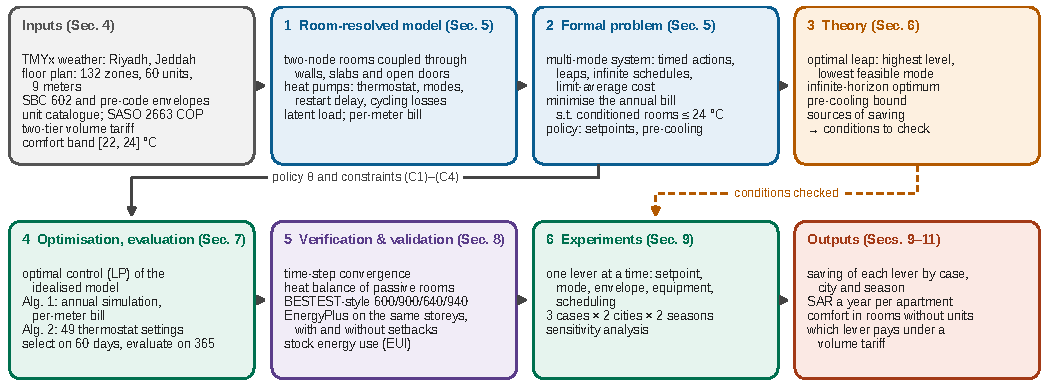
\includegraphics[width=\textwidth]{fig_pipeline}
\caption{Methodology. The inputs (Section~\ref{sec:context}) define a room-resolved model of the building (1), which is written as a multi-mode system and a bill-minimisation problem within a hard safe set (2, Section~\ref{sec:model}). The theory (3, Section~\ref{sec:theory}) characterises the optimal schedule and bounds what pre-cooling can gain; the computation (4, Section~\ref{sec:setup}) solves an idealised form of the problem as a perfect-foresight optimal-control program, and evaluates by annual simulation the pre-cooling settings a thermostat can realise. After the model is verified and validated (5, Section~\ref{sec:vv}), the experiments (6, Section~\ref{sec:results}) change one lever at a time and check the theory's conditions.}
\label{fig:pipeline}
\end{figure*}
\section{Case Study: Climate, Comfort and the Building}\label{sec:context}
The case study comprises two climates, a comfort band and one building, with its air-conditioners, its two envelopes and the three cases in which it is analysed. The model of Section~\ref{sec:model} is built on it, and all results are computed for it.

\subsection{Climate of Riyadh and Jeddah}\label{sec:weather}
The SBC divides the Kingdom into climate zones, and all Saudi cities are cooling-dominated~\citep{alayed2021thermal,stockmodel2020}. Riyadh and Jeddah are the two largest cities and lie in the two main residential climates, interior hot-dry and coastal hot-humid. Riyadh has large daily and seasonal swings, a small winter heating need and shoulder months close to the comfort band. Jeddah is warm and humid all year, so it needs cooling and dehumidification throughout, and its latent load is large where Riyadh's is negligible. Riyadh's cool winter also reveals the winter effect of the envelope, since insulation that helps in summer retains internal gains in winter as well. The pair therefore tests the levers in two different ways and shows whether the results hold across climates.

The model is driven by hourly weather for Riyadh and Jeddah from typical meteorological years (TMYx) assembled from weather-station records and the ERA5 reanalysis of the European Centre for Medium-Range Weather Forecasts (data sources in the Data availability statement). The files give dry-bulb and dew-point temperature, pressure, and global, direct and diffuse solar radiation, and they are the same files read by the EnergyPlus benchmark (Section~\ref{sec:validation}). Fig.~\ref{fig:weather} plots the three components that drive the model: air temperature against the comfort band, relative humidity and solar radiation. The monthly values are summarised in Appendix~\ref{app:S3} and tabulated in the repository. Riyadh is hot and dry: its monthly mean rises from $14.7\,^{\circ}$C in January to $36.4\,^{\circ}$C in July, with daily maxima above $43\,^{\circ}$C and relative humidity near $12\%$ in summer. Jeddah is milder but humid: its mean never falls below $23.5\,^{\circ}$C and its relative humidity stays between $54\%$ and $70\%$ all year. Both receive $4$--$8\,$kWh/m\textsuperscript{2} of solar radiation per day.


\begin{figure*}[t]
\centering
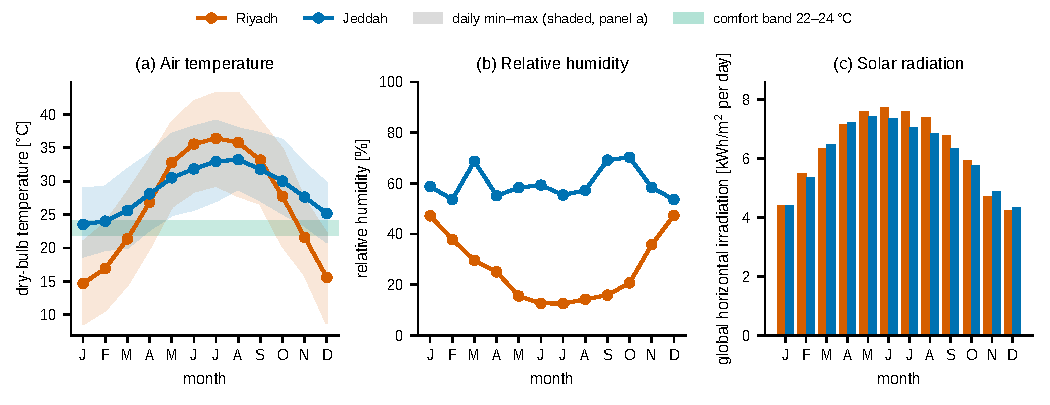
\includegraphics[width=\textwidth]{fig_weather}
\caption{Annual weather of Riyadh and Jeddah (TMYx typical years). (a)~Monthly mean air temperature and mean daily range against the comfort band: Riyadh crosses the band seasonally and exceeds $43\,^{\circ}$C on summer afternoons, while Jeddah's monthly mean never falls below it. (b)~Relative humidity: Riyadh is dry in summer and Jeddah humid all year, which drives its latent load. (c)~Daily solar irradiation, $4$--$8\,$kWh/m\textsuperscript{2} in both cities, which drives the solar gains.}
\label{fig:weather}
\end{figure*}

\subsection{Comfort range: ASHRAE, SBC and the one-sided ceiling}\label{sec:comfortrange}
ASHRAE~55 defines comfort through the predicted mean vote (PMV): a space complies when the PMV stays within $\pm0.5$, that is, at most $10\%$ predicted percentage dissatisfied (PPD)~\citep{standard55,ISO7730}. For summer clothing ($0.5\,$clo), light activity ($1.1$--$1.2\,$met), still air and $50\%$ relative humidity, this spans roughly $23$--$27\,^{\circ}$C of \emph{operative} temperature, and about $19$--$24\,^{\circ}$C in winter clothing ($1.0\,$clo). The SBC regulates the building fabric (Section~\ref{sec:stock}) rather than the setpoint, which is left to the occupant and to efficiency guidance.

We adopt a comfort band $[V_{\text{low}},V_{\text{high}}]=[22,24]\,^{\circ}$C of air temperature and treat its upper bound as a \emph{hard} ceiling rather than the centre of a symmetric deadband. There are three reasons for this choice in Saudi homes. First, in sunlit construction with warm inner surfaces the operative temperature exceeds the air temperature on summer afternoons, most in rooms under an uninsulated roof. In the insulated building studied here the excess is small (Section~\ref{sec:operative}), so a $24\,^{\circ}$C ceiling sits at or below the middle of the ASHRAE summer zone. In the uninsulated stock and under a roof, however, the excess moves a $24\,^{\circ}$C room towards the upper part of that zone, and letting rooms coast above the ceiling during the peak would take them towards its edge. The hard ceiling is therefore a conservative choice for the insulated building and a protective one for the stock. Second, at Jeddah's $54$--$70\%$ relative humidity (Fig.~\ref{fig:weather}b) evaporative cooling of the body is suppressed and the comfortable dry-bulb ceiling is lower still. Third, in the summer heat, conditioned rooms are refuges for vulnerable occupants. The ceiling also matches the lower end of the $24$--$26\,^{\circ}$C range recommended by efficiency guidance in the neighbouring Gulf state of Qatar~\citep{tarsheed_setpoint}. With this choice no saving is gained at the expense of comfort as measured by the air temperature of the conditioned rooms; the operative temperature it implies is checked in Section~\ref{sec:operative}. Humidity is priced through the latent load but not constrained (Section~\ref{sec:dynamics}). The safe set is imposed on the conditioned rooms, where occupants stay; the band is their comfort target. The passive zones, the rooms without a unit (Section~\ref{sec:passive}), are compared with the band but not constrained by the safe set, and Appendix~\ref{app:S1} reports how the controller brings them close to it.

Flexibility is therefore \emph{one-sided}. Both bounds of the safe set $[V_{\min},V_{\max}]=[20,24]\,^{\circ}$C are hard (Section~\ref{sec:problem}), so a controller may pre-cool into $[20,22)\,^{\circ}$C, below the band, but never let an occupied room rise above the ceiling. Every re-timing of cooling in this paper is thus a pre-cooling action (cool into the headroom, then return to the setpoint) and never an upward coast (illustrated in Section~\ref{sec:runex}). Since every room is taken to be occupied at all hours (A4), no room is allowed to float.

\subsection{The building: layout, air-conditioners, envelope and analysis cases}\label{sec:building}
The building studied is a four-storey apartment building with two apartments per floor, a common housing type in Saudi cities (Fig.~\ref{fig:layouts}). The building was designed for this study as a set of layered drawings in Drawing Exchange Format (DXF) (plans, section and elevation), with room sizes, wall types, storey height and stair dimensions that follow the SBC (Fig.~\ref{fig:layouts}a). Each apartment has a master bedroom with its own bath, two further bedrooms (Bed~2 and Bed~3), a living room open to a dining area and an enclosed west balcony, a kitchen, a guest room, three further baths, a maid room and circulation spaces (Appendix~\ref{app:S3} lists every room). The two apartments of a floor mirror each other about a common stair ($4.25\times9.05\,$m) on the south side, on a $19.15\times28.00\,$m footprint (Fig.~\ref{fig:layouts}b). Four floors of $3.40\,$m ($3.00\,$m clear) form the building, entered from the south (Fig.~\ref{fig:layouts}c). The top of the plan faces north. Apartments are numbered by storey, from 1 (ground) to 4 (top), with A on the west and B on the east.

Each room is one thermal zone of the model (Section~\ref{sec:prelim}), a rectangle (or union of rectangles) on the wall centrelines of the drawing, so that each zone's clear size is that of the drawing; the enclosed balcony is an unconditioned zone. Each window enters with its own width and orientation, which gives a window-to-wall ratio of $17.3\%$ for the building. The model derives each zone's floor area, its exterior walls and their orientations, and every shared wall and slab from the rectangles, so no adjacency is entered by hand. An apartment covers $231\,\text{m}^2$ on wall centrelines (without the balcony), a floor has $33$ zones and the building has $132$.

Every bedroom has its own split unit, as do the living room, the dining area, the kitchen and the guest room; each unit is chosen from a four-model product catalogue by rated coverage (Table~\ref{tab:acspec}; $1\,$ton $=3.517\,$kW of cooling). The drawing gives the living room and the dining area a unit each; together they cover $36\,\text{m}^2$, the upper limit of the largest unit's coverage, so one unit would have no margin. They are modelled as two zones joined by a $5.00\,$m opening. The baths, the maid room, the lobby, the corridor, the hall and the balcony have no unit. Interior doors are open, with the widths of the drawing ($0.70$--$0.90\,$m) and the $2.032\,$m minimum clear height of egress doors in SBC~201 (Section~1010)~\citep{sbc201_2018}; the wall-free openings of the open plan (corridor and hall to the living and dining area, living to dining) are $2.20$--$5.00\,$m wide and $3.00\,$m high. The apartment entrance and balcony doors are closed. The stair is conditioned and billed on a common meter, and each apartment has its own meter, to which the tariff applies. Each apartment therefore has seven units ($14.0\,$tons), and the building has $60$ units on nine meters.

The 1.5-, 2.0- and 2.5-ton units are inverter split heat pumps, modelled with four operating modes numbered $0$--$3$: off and three on modes (low, medium and high). The 3-ton unit is a fixed-speed rotary-compressor heat pump; its three fan speeds do not modulate the compressor, so it is modelled as an on/off unit that runs at full capacity whenever it runs. Sizing by rated coverage is how such units are chosen in practice; with the SBC envelope it leaves them several times larger than the peak load, and a right-sized alternative is tested in Section~\ref{sec:sensitivity}. Their efficiency is anchored to the air-conditioner standard of the Saudi Standards, Metrology and Quality Organization (SASO), SASO~2663, whose 2014 edition set a minimum split-unit energy efficiency ratio (EER) of $11.5\,$(Btu/h)/W at test condition T1~\citep{saso2663_2014}; the 2021 edition moved to seasonal ratings~\citep{saso2663}. At full load and the T1 rating condition ($35\,^{\circ}$C outdoors, $27\,^{\circ}$C indoors) the modelled COP is $3.37$, which equals an EER of $11.5$; at the $23.5\,^{\circ}$C reference setpoint it is $3.13$. The higher efficiency of the low and medium modes follows the assumed part-load ratios of Eq.~\eqref{eq:cop} (Section~\ref{sec:prelim}). The heating capacity of each unit is taken as $1.14$ times its cooling capacity ($6.0\,$kW for the $1.5$-ton unit), an assumed value.

\paragraph{Passive zones.}\label{sec:passive} About a third of each apartment's floor area has no unit: the four baths, the maid room, the lobby, the corridor, the entrance hall and the enclosed balcony. These \emph{passive zones} are cooled in summer and heated in winter only by the thermal shift from their neighbours (Section~\ref{sec:dynamics}). Their temperatures are therefore outputs of the model, not controlled quantities. Section~\ref{sec:passivetheory} states what they can reach, and Section~\ref{sec:comfortperf} reports them.

\begin{table}[!t]
\centering\footnotesize
\caption{Air-conditioner catalogue and the rooms each unit serves. All units are split heat pumps for heating and cooling. The 1.5- to 2.5-ton units are inverter units with four operating modes (off, low, medium, high; capacity fractions $0$, $0.35$, $0.65$ and $1$); the 3-ton unit has a fixed-speed rotary compressor and runs on/off at full capacity. Capacity: cooling/heating; coverage: rated floor area. The 2.0-ton unit serves no room of the plan. The stair ($38.5\,\text{m}^2$) lies just above the rated coverage of its unit, and the dining area ($11.0\,\text{m}^2$) below that of the smallest unit.}
\label{tab:acspec}
\setlength{\tabcolsep}{3pt}
\begin{tabularx}{\linewidth}{@{}l l l R@{}}
\toprule
Unit & Capacity [kW] & Coverage & Rooms served \\
\midrule
1.5 ton & $5.28$/$6.0$ & $16$--$18\,\text{m}^2$ & Bed~2, Bed~3, kitchen, dining area \\
2.0 ton & $7.03$/$8.0$ & $19$--$22\,\text{m}^2$ & none \\
2.5 ton & $8.79$/$10.0$ & $22$--$30\,\text{m}^2$ & master bedroom, living room \\
3.0 ton & $10.55$/$12.0$ & $30$--$36\,\text{m}^2$ & guest room, stair \\
\bottomrule
\end{tabularx}
\end{table}

\begin{figure*}[!t]
\centering
\newlength{\cadW}\setlength{\cadW}{0.31\textwidth}\newlength{\cadH}\setlength{\cadH}{0.40\textwidth}%
\newcommand{\cadpanel}[1]{{\setlength{\fboxsep}{0pt}\setlength{\fboxrule}{0.4pt}\fcolorbox{black!35}{white}{\parbox[c][\cadH][c]{\cadW}{\centering\includegraphics[width=0.94\cadW,height=0.96\cadH,keepaspectratio]{#1}}}}}%
\begin{subfigure}[b]{0.32\textwidth}\centering\cadpanel{fig_cad_apartment}\caption{Case~1: apartment~A}\end{subfigure}\hfill
\begin{subfigure}[b]{0.32\textwidth}\centering\cadpanel{fig_cad_floor}\caption{Case~2: typical floor}\end{subfigure}\hfill
\begin{subfigure}[b]{0.32\textwidth}\centering\cadpanel{fig_cad_elevation}\caption{Case~3: elevation and section}\end{subfigure}
\caption{The building analysed in the three cases (drawings generated as layered DXF files; clear dimensions in metres). (a)~Apartment~A, analysed alone in Case~1. (b)~The typical floor: two mirror-image apartments around the common stair; north is up. (c)~South elevation (top) and section A--A through the stair (bottom) of the four-storey building (floor-to-floor height $3.40\,$m, $3.00\,$m clear; windows from $0.90$ to $2.40\,$m above each floor). The zone rectangles of the model follow the wall centrelines of (b).}
\label{fig:layouts}
\end{figure*}

\paragraph{Envelope.}\label{sec:stock} SBC~602 is the Kingdom's energy-conservation code for low-rise residential buildings~\citep{sbc602_2018}. It sets the envelope performance (wall, roof and glazing U-values and the glazing solar heat gain) for three climate zones~\citep{alayed2021thermal,stockmodel2020}. The walls, roof and glazing of the building meet the residential requirements for climate Zone~1 (SBC~602, as tabulated by \citet{stockmodel2020}), the hottest zone, which includes Riyadh. We apply the same requirements in both cities as a common reference: a wall U-value of $0.34\,\text{W/m}^2\text{K}$~\citep{sbc602_2018,alayed2021thermal,stockmodel2020}, roof and window U-values of $0.20$ and $2.67\,\text{W/m}^2\text{K}$ and a glazing solar heat-gain coefficient (SHGC) of $0.25$~\citep{stockmodel2020}, with the windows of the drawing. Partitions and floor slabs keep the uninsulated U-values of the existing stock, and the ground slab is uninsulated (Table~\ref{tab:params}). This SBC-compliant building is the main case of the study. To quantify the value of the code, the same building is also simulated with the envelope of the existing, largely uninsulated stock: wall, roof and window U-values of $2.146$, $2.123$ and $5.778\,\text{W/m}^2\text{K}$ and an SHGC of $0.62$, taken from the calibrated model of an existing Riyadh residence~\citep{alyami2021building}. Nothing else is changed, so the difference isolates the envelope.

\paragraph{Analysis cases.}\label{sec:steps} The same building is analysed as three cases of increasing extent (Fig.~\ref{fig:layouts}). \emph{Case~1} is one apartment on its own, apartment~A of an intermediate storey (Fig.~\ref{fig:layouts}a). This is the dwelling that receives a household bill. Its walls and slabs shared with the other apartment, the core and the storeys above and below face conditioned space and are treated as adiabatic. \emph{Case~2} is the typical floor (Fig.~\ref{fig:layouts}b): both apartments side by side and the core, with the heat exchange between them. Its slabs remain adiabatic. \emph{Case~3} is the whole building (Fig.~\ref{fig:layouts}c): four storeys of two apartments, with ground contact on the lowest storey, the roof above the highest, and heat exchange through every slab. Where Case~3 results are given for one apartment, it is 2A, on the first storey above the ground, which is neither in contact with the ground nor under the roof. Each case is run in both cities, for both envelopes (SBC-compliant and pre-code, Section~\ref{sec:stock}), over the whole TMYx year, so both summer cooling and winter heating are simulated.
\section{Model and Problem Formulation}\label{sec:model}
Here the building of Section~\ref{sec:context} is cast as a formal model, and the optimisation problem is stated. The formulation uses the multi-mode formalism of \citet{alur2012optimal}, \citet{wojtczak2013optimal} and \citet{mousa2017optimal} and the coupled-zone model of \citet{nghiem2012scalable}. Only the parts the theory needs are stated here, and the full formal definitions (zone network, multi-mode system, timed actions, schedules, runs and their costs, schedulability) with the continuations of the running example are in Appendix~\ref{app:S4}.

\subsection{Modelling assumptions}\label{sec:assumptions}
The theory of Section~\ref{sec:theory} rests on five assumptions, of which the simulation relaxes the first three. \textbf{(A1)}~Each zone is well mixed; the theory reads it as one lumped temperature $V_i$, the simulation as two nodes, air and structure (Section~\ref{sec:dynamics}). \textbf{(A2)}~The COP is quasi-static, a function of mode and ambient temperature (Eq.~\eqref{eq:cop}) with no cycling loss; the simulation adds its dependence on the indoor air, cycling losses, standby power and capacity derating (Section~\ref{sec:params}). \textbf{(A3)}~Within one leap cycle the heat gain $L$ and the ambient temperature are constant. This holds only roughly for a lightly loaded room, whose cycle can last hours (about $\exCycleHr\,$h for the running example), so applying the cycle results hour by hour is an approximation; the simulation does not use (A3). \textbf{(A4)}~Every room of every apartment is occupied and conditioned at all hours, with every conditioned zone following the same policy, so adjacent conditioned zones operate at the same level; the conclusions inherit this idealisation (Section~\ref{sec:limitations}). \textbf{(A5)}~Building properties that are uncertain in practice (window sizes and U-values, solar absorptance, internal gains, interior doors all open) are held at the values of the drawing and of Table~\ref{tab:params}; the absorptance, internal gains and door schedules are varied in Section~\ref{sec:sensitivity}, and the windows only through the two envelopes compared.

\subsection{Zones, units and the multi-mode system}\label{sec:prelim}
The building is a finite set of zones $\mathcal{Z}=\{1,\dots,N\}$ (rooms). The \emph{conditioned} zones $\mathcal{Z}_c$ each have their own unit; the \emph{passive} zones $\mathcal{Z}_u$ (baths, maid room, lobby, corridor, hall and enclosed balcony) have none. Zone $i$ has a thermal capacitance $C_i$ and a temperature $V_i(t)$; adjacent zones $i\ne j$, sharing a partition or slab, are coupled by the conductance $K_{ij}=K_{ji}$ (U-value times area, zero otherwise), and each zone exchanges heat with the outdoors through $K^{\mathrm{env}}_i$ (infiltration alone for interior zones).

Each conditioned zone is served by a split heat-pump unit with four modes $M=\{0,1,2,3\}$ (off, low, medium, high; a fixed-speed unit has only $0$ and $3$). In mode $m$ it removes heat at the rate $f_m\psi(T_a)Q_i$ when cooling and adds $f_mQ^{\mathrm{h}}_i$ when heating, where $Q_i$ is its rated cooling capacity, $\psi(T_a)=[1-0.01(T_a-35)]_{0.8}^{1.1}$ derates it with the outdoor temperature, $Q^{\mathrm{h}}_i=1.14\,Q_i$, and $0=f_0<f_1<f_2<f_3=1$ are the capacity fractions ($0.35$, $0.65$, $1$). It draws $f_m\psi Q_i/\mathrm{COP}_m$ when cooling and $f_mQ^{\mathrm{h}}_i/\mathrm{COP}_m$ when heating, with
\begin{subequations}\label{eq:cop}
\begin{align}
\mathrm{COP}^{\text{cool}}_m(T_a,V_i)&=c_m\,\varphi(T_a)\,g(V_i),\quad \mathrm{COP}^{\text{heat}}_m=h_m,\\
\varphi(T_a)&=\bigl[1-0.02\,(T_a-27)\bigr]_{0.60}^{1.15},\\
g(V_i)&=\bigl[1-\gamma\,(27-V_i)\bigr]_{0.8}^{1.1},\quad \gamma=0.02\,\text{K}^{-1},
\end{align}
\end{subequations}
where $[x]_a^b=\min\{b,\max\{a,x\}\}$, $c_1=5.81>c_2=4.98>c_3=4.01$ and $h_1=4.6>h_2=4.0>h_3=3.2$: a unit is most efficient at low output. The cooling coefficients are anchored to the Saudi efficiency minimum (Section~\ref{sec:building}); $\varphi$ lowers the COP as the outdoor air warms and $g$ as the room's air falls below the $27\,^{\circ}$C rating condition ($g=0.93$ at $23.5\,^{\circ}$C; $\gamma$ is assumed and varied in Section~\ref{sec:sensitivity}). The building is then a multi-mode system~\citep{mousa2017optimal} with one mode per unit, the heat balance of Eq.~\eqref{eq:heat} as rate function, a cost $\pi_i(m)$ per unit time for each unit and mode, the safe set $\mathcal{S}=[V_{\min},V_{\max}]$ and an initial state $V_0$.

\subsection{Thermal dynamics: inter-zone coupling and latent load}\label{sec:dynamics}
Following \citet{nghiem2012scalable} and the two-node simplification of ISO~13790~\citep{iso13790_2008}, each zone has an air node $V_i$, which the thermostat senses and the unit acts on, and a structure node $W_i$, the inner layers of its walls and slabs:
\begin{subequations}\label{eq:heat}
\begin{align}
C^{\mathrm{a}}_i\dot V_i&=K^{\mathrm{w}}_i(T_a-V_i)+K^{\mathrm{am}}_i(W_i-V_i)+\textstyle\sum_{j\in\mathcal{D}_i}q_{ji}\nonumber\\
&\quad+(1-f_r)G_i-S^{\mathrm{sky}}_i-s_i\,\beta_i\,f_{u_i}\hat Q_i,\label{eq:heat-a}\\
C^{\mathrm{m}}_i\dot W_i&=q^{\mathrm{env}}_i+\textstyle\sum_{j\ne i}K_{ij}(W_j-W_i)+K^{\mathrm{am}}_i(V_i-W_i)\nonumber\\
&\quad+S^{\mathrm{w}}_i+f_rG_i,\label{eq:heat-b}\\
q^{\mathrm{env}}_i&=K^{\mathrm{o}}_i(T_a-W_i)+S^{\mathrm{o}}_i+K^{\mathrm{grd}}_i(T_g-W_i).\label{eq:heat-c}
\end{align}
\end{subequations}
Here $K^{\mathrm{w}}_i$ covers windows and infiltration ($n_{\mathrm{ach}}=0.4$ air changes per hour, ACH), $K^{\mathrm{am}}_i$ joins air and structure, $\mathcal{D}_i$ are the rooms joined by an open door (Eq.~\eqref{eq:door}), $G_i$ are the internal gains with radiant share $f_r$, $S^{\mathrm{sky}}_i$ is the long-wave loss of the windows and $S^{\mathrm{w}}_i$ the window solar gain (SHGC with angle-dependent transmission~\citep{ashrae_fund2021}). $S^{\mathrm{o}}_i$ is the sol-air excess of walls and roof, net of the sky loss $\varepsilon F_{\text{sky}}(\sigma_{\text{SB}}T_a^4-I_{\text{IR}})$ with the hourly infrared sky radiation $I_{\text{IR}}$ of the weather file, the Stefan--Boltzmann constant $\sigma_{\text{SB}}$, $\varepsilon=0.9$ and $F_{\text{sky}}=1$ (roof) or $0.5$ (walls, windows)~\citep{iso13790_2008}. $T_a$ and $T_g$ are the ambient and ground temperatures ($K^{\mathrm{grd}}_i\ne0$ on the ground storey only), $u_i(t)\in M$ is the unit's mode ($u_i\equiv0$ in passive zones), $s_i=\pm1$ for cooling or heating, $\beta_i\in[0,1]$ the fraction of the step the unit runs, and $\hat Q_i$ is $\psi(T_a)Q_i$ in cooling and $Q^{\mathrm{h}}_i$ in heating. Apart from the door exchange the rates are affine in the temperatures, so the building is close to a linear-rate multi-mode system~\citep{wojtczak2013optimal}.

Through a door of width $W_d$ and height $H_d$, buoyancy carries the heat~\citep{brown1962natural}
\begin{equation}\label{eq:door}
q_{ji}=\rho c_p\,\tfrac{C_{\mathrm{dis}}}{3}W_d\sqrt{\tfrac{g_0H_d^3}{\bar T}}\;(V_j-V_i)\,|V_j-V_i|^{1/2}
\end{equation}
from room $j$ into room $i$ ($C_{\mathrm{dis}}=0.6$, $\bar T=297\,$K, $\rho$ and $c_p$ the density and specific heat of air, $g_0$ the gravitational acceleration); at $1\,$K a $0.90\,$m door carries about $110\,$W, several times more than a partition wall. We call the exchange through walls, slabs and doors the \emph{thermal shift} between rooms; because $K_{ij}=K_{ji}$ and $q_{ji}=-q_{ij}$, it moves heat between rooms without creating or removing it.

Humid infiltration air imposes a latent load on each conditioned zone whenever the outdoor humidity ratio $\omega_a$ exceeds the indoor target $\omega^\ast=9.6\,$g/kg ($55\%$ relative humidity at $23\,^{\circ}$C, below $60\%$ everywhere in the band, and independent of the setpoint):
\begin{equation}\label{eq:latent}
L^{\mathrm{lat}}_i = \tfrac{n_{\mathrm{ach}}}{3600}\, \rho\, \mathrm{Vol}_i\, \max(\omega_a - \omega^\ast,\,0)\, h_{fg},
\end{equation}
with the zone's air volume $\mathrm{Vol}_i$ and the latent heat $h_{fg}$. The target is assumed met, the latent electricity is priced at a fixed latent COP, internal moisture is omitted and passive zones are not dehumidified; these assumptions are tested in Section~\ref{sec:sensitivity}.

\subsection{Parameters and their provenance}\label{sec:params}
Every parameter is fixed a priori from the code, the product catalogue, the floor plan, the weather file, cited statistics or a stated nominal value (Table~\ref{tab:params}); none is fitted to the quantities against which the model is later checked. Each conductance is a U-value times an area from the plan (storey height $3.40\,$m, clear height $3.00\,$m), and capacitance, internal gains and latent air mass scale with floor area. The capacitance, $270\,$kJ/(m$^2$K) of floor, lies close to the heavy-class default of ISO~13790 ($260$)~\citep{iso13790_2008}, whose reduced-order room model remains the usual choice at this scale although the standard has been superseded by ISO~52016-1. A share of $5\%$ of the capacitance sits on the air node (our choice, since the standard's air node is massless), the air--structure coupling is given by the ISO surface coefficients in series, and half of the internal gains are radiant. Internal gains average $5.4\,\text{W/m}^2$ with an afternoon peak, derived from the Saudi end-use split~\citep{stockmodel2020}, raised in the kitchen and reduced in baths and circulation. The ground slab follows ISO~13370~\citep{iso13370_2017} against the monthly ground temperature of the weather file. Each unit draws $3\,$W on standby, and its hourly electricity is divided by the part-load factor $\mathrm{PLF}=1-C_d(1-\mathrm{RTF})$, where RTF is the fraction of the hour it runs. The coefficient is $C_d=0.25$ for the fixed-speed units, the rating default for single-speed equipment~\citep{ahri210240}, and an assumed $C_d=0.15$ for the inverter units, which cycle at or below their minimum speed; both are varied in the sensitivity and uncertainty analyses (Section~\ref{sec:sensitivity}). The rated COPs include the indoor fan, which runs only with the compressor.

\begin{table*}[t]
\centering
\caption{Parameters and their provenance. Compliant envelope: Saudi residential requirements for climate Zone~1~\citep{sbc602_2018,stockmodel2020,alayed2021thermal}; pre-code: calibrated model of an existing Saudi residential building~\citep{alyami2021building}. Each conductance is $K=UA/1000$ [kW/K] with $A$ from the floor plan.}
\label{tab:params}
\footnotesize
\begin{tabularx}{\linewidth}{L{4.6cm} l l R}
\toprule
Quantity & SBC & Pre-code & Source / justification \\
\midrule
Wall / roof / window U [W/m\textsuperscript{2}K] & 0.34 / 0.20 / 2.67 & 2.146 / 2.123 / 5.778 & SBC Zone~1~\citep{stockmodel2020}; existing stock~\citep{alyami2021building} \\
Glazing SHGC & 0.25 & 0.62 & SBC Zone~1~\citep{stockmodel2020}; existing stock~\citep{alyami2021building} \\
Exterior wall incl.\ $17.3\%$ glazing [W/m\textsuperscript{2}K] & 0.74 & 2.78 & derived (area-weighted, building mean) \\
Partition / slab U [W/m\textsuperscript{2}K] & \multicolumn{2}{c}{1.728 / 2.047} & existing stock~\citep{alyami2021building} \\
Ground slab U [W/m\textsuperscript{2}K]; ground temperature & \multicolumn{2}{c}{0.40;\ monthly, 2\,m} & ISO~13370~\citep{iso13370_2017}, uninsulated slab; TMYx ground record \\
Capacitance $C$ [kWh/K per 20\,m\textsuperscript{2}] & \multicolumn{2}{c}{1.5 ($270\,$kJ/(m\textsuperscript{2}K))} & heavy class of ISO~13790~\citep{iso13790_2008}; block/concrete construction \\
Air-node share of $C$; air--structure coupling & \multicolumn{2}{c}{$5\%$;\ $9.9\,$W/m\textsuperscript{2}K of floor} & ISO~13790 two-node simplification, heavy class~\citep{iso13790_2008} \\
Infiltration $n_{\mathrm{ach}}$ [ACH] & \multicolumn{2}{c}{0.4} & nominal, new construction (stock: 0.8~\citep{stockmodel2020}); sensible and latent \\
Interior doors / openings $W_d\times H_d$ [m]; $C_{\mathrm{dis}}$ & \multicolumn{2}{c}{$0.70$--$0.90\times2.032$ / $2.20$--$5.00\times3.00$;\ 0.6} & drawing; height SBC~201~\citep{sbc201_2018}; \citet{brown1962natural} \\
Internal gains [W/m\textsuperscript{2}]: continuous + daytime half-sine; mean & \multicolumn{2}{c}{$\hlGainBase$ + $0$--$\hlGainAmp$ ($\hlGainOn$--$\hlGainOff$, peak $\hlGainPk$); $5.4$} & end-use split~\citep{stockmodel2020}; times a room factor of $0$--$1.5$ by use, assumed (Appendix~\ref{app:S3}) \\
Opaque solar absorptance & \multicolumn{2}{c}{0.7} & nominal (idealised, A5) \\
Exterior film / ground reflectance & \multicolumn{2}{c}{17\,W/m\textsuperscript{2}K / 0.2} & nominal (sol-air temperature and diffuse gains) \\
Sky long-wave: $\varepsilon$; $F_{\text{sky}}$ roof / walls, windows & \multicolumn{2}{c}{0.9;\ 1 / 0.5} & ISO~13790~\citep{iso13790_2008}; hourly infrared radiation of the TMYx file \\
Window solar & \multicolumn{2}{c}{angle-dependent} & normalised SHGC curve of double glazing~\citep{ashrae_fund2021} \\
Unit sizes [ton] & \multicolumn{2}{c}{1.5 / 2.0 / 2.5 / 3.0} & catalogue, by coverage (Table~\ref{tab:acspec}) \\
Mode capacity fractions $f_1/f_2/f_3$ & \multicolumn{2}{c}{0.35 / 0.65 / 1.0} & inverter units (Eq.~\eqref{eq:cop}); fixed-speed: $f_3$ only \\
Cycling degradation $C_d$: inverter / fixed-speed & \multicolumn{2}{c}{0.15 / 0.25} & part-load factor per hour; inverter assumed, fixed-speed \citet{ahri210240} \\
Standby power; capacity derating & \multicolumn{2}{c}{3\,W per unit;\ $\mp1\%$/K about $35\,^{\circ}$C, $[0.8,1.1]$} & nominal \\
Restart delay; mode escalation & \multicolumn{2}{c}{3\,min;\ $0.4$/$1.0\,$K, full if lagging} & anti-short-cycle timer; nominal \\
Thermostat differential; setpoint step & \multicolumn{2}{c}{1.0\,K;\ 0.5\,K} & typical room thermostat; state updated every 3 min \\
Cooling COP (modes 1/2/3) & \multicolumn{2}{c}{$5.81/4.98/4.01\times\varphi(T_a)\,g(V)$} & SASO~2663 minimum at full load~\citep{saso2663_2014}; ratios and $\gamma$ assumed, Eq.~\eqref{eq:cop} \\
Heating COP (modes 1/2/3) & \multicolumn{2}{c}{4.6 / 4.0 / 3.2} & nominal heat-pump values \\
Heating / cooling capacity $Q^{\mathrm{h}}_i/Q_i$ & \multicolumn{2}{c}{1.14} & nominal inverter heat pump ($6.0$ vs $5.28\,$kW at $1.5\,$ton) \\
Latent (dehumidification) COP, $\mathrm{COP}_{\mathrm{lat}}$ & \multicolumn{2}{c}{3.4} & nominal, all modes (Eq.~\eqref{eq:latent}) \\
Reference setpoints: cooling / heating [$^\circ$C] & \multicolumn{2}{c}{23.5 / 22.5} & ceiling and band floor $\mp$ half the differential \\
Indoor humidity target $\omega^\ast$ & \multicolumn{2}{c}{$9.6\,$g/kg} & $55\%$ relative humidity at $23\,^{\circ}$C; within the $12\,$g/kg applicability limit of the ASHRAE~55 graphic method~\citep{standard55} \\
Weather & \multicolumn{2}{c}{TMYx hourly} & typical year from station records and ERA5 (Fig.~\ref{fig:weather}; Appendix~\ref{app:S3}) \\
\bottomrule
\end{tabularx}
\end{table*}

\subsection{Leap cycles, levels and the comfort frontier}\label{sec:runex}
A unit's operation is a \emph{schedule} of \emph{timed actions} $(m,t)$, each keeping the unit in mode $m$ for a time $t$; it is \emph{safe} if its run, the sequence of states it produces from the initial state, stays in $\mathcal{S}$, and its cost is the energy price times its long-run mean electrical power $J_\infty$~\citep{mousa2016optimal,mousa2017optimal,alur2012optimal}. The theory needs one kind of schedule (Fig.~\ref{fig:defs}).

\begin{figure}[t]
\centering
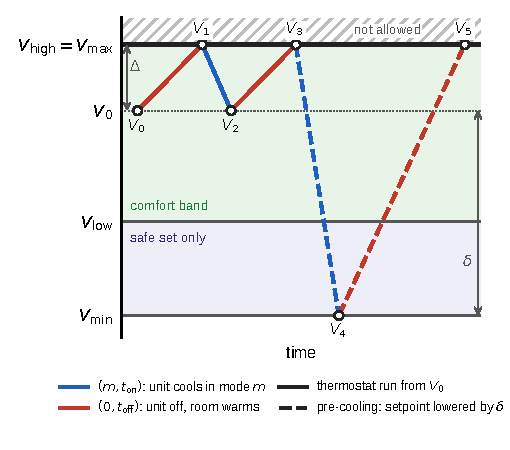
\includegraphics[width=\columnwidth]{fig_defs}
\caption{Leap cycles (schematic). The comfort band $[V_{\text{low}},V_{\text{high}}]$ lies inside the safe set $[V_{\min},V_{\max}]$ with a hard ceiling, $V_{\text{high}}=V_{\max}$. The labels $V_0,\dots,V_5$ are successive states of one zone's run, starting from the initial state $V_0$, the thermostat's lower switching point: drifts $(0,t_{\mathrm{off}})$ (red) and cooling leaps $(m,t_{\mathrm{on}})$ (blue) form a leap cycle of amplitude $\Delta$ under the ceiling. Pre-cooling lowers the setpoint by $\delta$ (dashed), at most to $V_{\min}+0.5\,$K, so that the thermostat's lower switching point stays at or above the floor $V_{\min}$.}
\label{fig:defs}
\end{figure}

\begin{definition}[Leap cycle, level, schedulability and comfort frontier]\label{def:optleap}\label{def:sched}
Let a conditioned zone in the cooling season have heat gain $L(V)$, the net heat entering it per unit time with its unit off. A \emph{leap cycle} of amplitude $\Delta>0$ under a top temperature $V^{\top}$ is a drift $(0,t_{\mathrm{off}})$ from $V^{\top}-\Delta$ up to $V^{\top}$ followed by a cooling leap $(m,t_{\mathrm{on}})$ back down; repeated for ever, it is an infinite schedule. Its \emph{level} $\bar V$ is its time-mean temperature, about $V^{\top}-\Delta/2$. The zone is \emph{schedulable} in mode $m$ if $f_m\psi Q_i>L(\bar V)$, so that the mode can bring it back; this is the zero-sum dwell-time condition of \citet{alur2012optimal} for one zone, with \emph{duty} $d_m=L/(f_m\psi Q_i)<1$ and utilisation $U_i=L/Q_i$. The \emph{comfort frontier} $\bar V^\ast$ is the highest level whose cycle stays at or below $V_{\text{high}}$. In the heating season drift and leap exchange roles.
\end{definition}

\begin{runex}
Bed~2 of apartment 2A (Section~\ref{sec:building}, Fig.~\ref{fig:layouts}a), $\exArea\,\text{m}^2$ on the north side next to the party wall, has one exterior wall and a $1.5$-ton unit ($Q=5.28\,\text{kW}$). With the SBC envelope, $C=\exC\,\text{kWh/K}$ and $K^{\mathrm{env}}=\exKenv\,\text{W/K}$ (wall and window \exKwall, infiltration \exKinf), while its six neighbours are coupled to it by $\exKtot\,\text{W/K}$, about \exKratio\ times its envelope conductance. In mean July conditions in Riyadh ($T_a=\exTa\,^{\circ}$C), read as one lumped room at a level of $23.5\,^{\circ}$C, it gains $L=\exL\,\text{kW}$ (conduction and infiltration \exLcond, internal gains \exG, solar minus sky loss \exS; the conditioned neighbours, at the same level, add no net heat). With its unit off, it warms at $\exWarm\,\text{K/h}$; mode~1 removes $\exQone\,\text{kW}$ and cools it at $\exCoolRate\,\text{K/h}$, with duty $d_1=\exU$. For the $1\,$K differential one leap cycle is $\langle(0,\exToff\,\text{min}),(1,\exTon\,\text{min})\rangle$.
\end{runex}

\subsection{The Saudi two-tier tariff}\label{sec:tariff}
The electrical power of unit $i$ is $P_i(t)=f_{u_i(t)}\hat Q_i/\mathrm{COP}_{u_i(t)}$ (Eq.~\eqref{eq:cop}) plus its latent share. A metering map $\mu$ assigns every unit to the meter that bills it, one per apartment and one common meter for the stair, and meter $r$ uses $E_{r,k}=\int_{\text{month }k}\sum_{i:\mu(i)=r}P_i(t)\,dt$ in month $k$. The residential tariff, set by the Saudi Electricity Regulatory Authority and billed by the Saudi Electricity Company, is a two-tier \emph{volume} tariff applied to each meter separately~\citep{sec_tariff}:
\begin{subequations}\label{eq:tariff}
\begin{align}
\Pi^{\text{vol}}&=1.15\sum_{r=1}^{R}\sum_{k=1}^{12}b(E_{r,k}),\label{eq:tariff-a}\\
b(E)&=0.18\min(E,6000)+0.30\,(E-6000)^{+},\label{eq:tariff-b}
\end{align}
\end{subequations}
in Saudi riyals (SAR) a year, where $(x)^{+}=\max(x,0)$ and $1.15$ adds the $15\%$ value-added tax (VAT). The tariff prices energy alone: it has no time-of-use component, no demand charge and, unlike the multi-mode costs of \citet{mousa2017optimal}, no charge per switch; the energy a unit loses by cycling is counted through the part-load factor. Fixed meter charges are excluded. For a meter in tier~1, as every meter of the SBC-compliant building is (Section~\ref{sec:comfortperf}), the price is $\lambda=0.207\,$SAR/kWh (US\$0.055/kWh at the pegged rate of SAR~3.75 per US\$, used throughout), the cost of unit $i$ in mode $m$ is $\pi_i(m)=\lambda f_m\psi(T_a)Q_i/\mathrm{COP}_m(T_a)$, and the bill is the sum of the costs of the units' schedules.

\begin{runexc}
Apartment 2A of the SBC-compliant building in Riyadh (Case~3) uses $\exAptKwh\,$kWh of HVAC electricity a year at the reference setpoints, never more than $\exAptMaxMonth\,$kWh in a month, so even if HVAC were only a third of its use, the meter would stay in tier~1. Its HVAC bill is $\exAptKwh\times0.207\approx\exAptBill\,$SAR, and any policy's bill is proportional to its energy.
\end{runexc}

\subsection{Controller}\label{sec:controller}
Choosing every unit's timed actions directly would be a combinatorial problem over $|M|^{|\mathcal{Z}_c|}$ mode vectors per step. Instead, every unit applies one compact \emph{policy} $\theta=(V^{\text{cool}},\allowbreak V^{\text{heat}},\allowbreak\delta_{\text{night}},\allowbreak\delta_{\text{peak}})$ to its zone: cooling and heating setpoints and the depth pair $\delta=(\delta_{\text{night}},\delta_{\text{peak}})$ by which the cooling setpoint is lowered from 22:00 to 06:00 (night pre-cooling) and from 10:00 to 13:00 (pre-peak pre-cooling). Setpoints and depths move in $0.5\,$K steps. Each unit is controlled by an on/off thermostat with a $1\,$K differential centred on its active setpoint (in cooling: on at the setpoint plus $0.5\,$K, off at the setpoint minus $0.5\,$K), with the switching instant resolved within the $3$-minute step and at most one change of state per step, which also gives the usual $3$-minute restart delay. While on, an inverter unit chooses its mode from the rise its room's air would make within the step without cooling. This rule idealises the units' own logic, which manufacturers do not publish: low by default, medium if that rise would reach $0.4\,$K above the switch-on point, high if it would reach $1.0\,$K, and full capacity if its room is still above the switch-on point at the start of a step; a fixed-speed unit runs at full capacity. Heating works in the same way about the heating setpoint.

The units follow the usual seasonal changeover. In months whose mean air temperature is below the band floor $V_{\text{low}}$ (November to March in Riyadh; none in Jeddah), they heat and cool automatically, with the active heating setpoint at least $1\,$K below the active cooling setpoint. In the other months they cool, and heat only as a \emph{floor guard}: a low-limit heating setpoint of $21\,^{\circ}$C (on at $20.5$, off at $21.5\,^{\circ}$C), capped at $1\,$K below the active cooling setpoint. Pre-cooling acts only in cooling mode, with depths capped so that the cooling setpoint never falls below $V_{\min}+0.5\,$K; the controller therefore never cools a room below $V_{\min}$. Under the reference and ordinary policies, the guard holds the floor: without it, rooms of the uninsulated pre-code building fall below $V_{\min}$ ($\hlGuardColdR\,$K$\cdot$h a year in Riyadh; $\hlGuardColdJ\,$K$\cdot$h and down to $\hlGuardMinJ\,^{\circ}$C in Jeddah); it never acts in the SBC-compliant building at the reference policy. Its electricity is booked as heating energy of the month in which it acts and is part of the HVAC bill; in the pre-code building in Jeddah, which has no heating months, it adds $\hlGuardHeatJ\,$kWh of heating a year (about $\hlGuardHeatPctJ\%$ of the building's HVAC electricity), and with the small change in cooling that follows it raises the annual bill by $\hlGuardBillJ\%$ (full-year runs). During deep night pre-cooling (cooling setpoint $20.5$--$21.5\,^{\circ}$C), however, the cap moves the guard's switch-on point below $20.5\,^{\circ}$C, and a room can still drift below $20\,^{\circ}$C on a cool night, as it does under some deep night pre-cooling policies of the pre-code building in Jeddah. Other pre-cooling policies of the pre-code building, in both cities, let a room pass the ceiling. All such policies are inadmissible and are excluded. Each unit needs only its own zone temperature and the clock, and the policy induces for every unit an infinite schedule of leap cycles. With $\delta=(0,0)$ the controller is an ordinary thermostat.

\subsection{The optimisation problem, feasibility and admissibility}\label{sec:optproblem}\label{sec:problem}
The problem, in the form of \citet{mousa2017optimal}, is to choose the policy that minimises the annual bill:
\begin{alignat}{2}
&\min_{\theta}&\quad&\Pi(\theta)=\Pi^{\text{vol}}\bigl(\{E_{r,k}(\theta)\}\bigr)\label{eq:obj}\\
&\text{s.t.}&&\text{(C0) }u_i(t)=\kappa_\theta\bigl(V_i,t\bigr)\ \ \forall i\in\mathcal{Z}_c,\nonumber\\
&&&\text{(C1) Eqs.~\eqref{eq:heat}--\eqref{eq:latent} hold }\forall i\in\mathcal{Z},\nonumber\\
&&&\text{(C2) }V_i(t)\le V_{\text{high}}=24\,^{\circ}\text{C}\ \ \forall i\in\mathcal{Z}_c,\nonumber\\
&&&\text{(C3) }V_i(t)\ge V_{\min}=20\,^{\circ}\text{C}\ \ \forall i\in\mathcal{Z}_c,\nonumber\\
&&&\text{(C4) }u_i(t)\in M\ \forall i\in\mathcal{Z}_c;\ \ u_i\equiv0\ \forall i\in\mathcal{Z}_u,\nonumber\\
&&&\text{(C5) }V^{\text{heat}}=V_{\text{low}}+\Delta_{\text{th}}/2=22.5\,^{\circ}\text{C},\nonumber
\end{alignat}
for all times $t$. (C0) states that each unit's mode is set by the controller $\kappa_\theta$ of Section~\ref{sec:controller} under policy $\theta$ from its own zone temperature and the clock, (C1) the dynamics, (C2) the comfort ceiling, (C3) the safe floor, (C4) the finite modes and (C5) the heating setpoint, fixed at the comfort target of the heating months (the band floor plus half the differential $\Delta_{\text{th}}=1\,$K). The heating setpoint is therefore not a decision variable: without (C5) a colder heating setpoint, which keeps rooms within the safe set but below the band in winter, would be counted as a saving. The decision variables are the cooling setpoint and the depth pair.

\paragraph{Admissibility.} The safe set $[V_{\min},V_{\max}]=[20,24]\,^{\circ}$C is hard for every policy, at its ceiling and at its floor. A policy is \emph{admissible} if every conditioned zone stays within it at every step of the simulated year: the excursions above the ceiling, $\sum_i\int\max(V_i-V_{\text{high}},0)\,dt$, and below the floor, $\sum_i\int\max(V_{\min}-V_i,0)\,dt$, must both be zero up to floating-point round-off. Every other policy is excluded, and problem~\eqref{eq:obj} asks for the cheapest admissible policy. The band floor $V_{\text{low}}=22\,^{\circ}$C is the comfort target rather than a constraint on the air temperature: in the heating months it is held by the heating setpoint of (C5), and in the cooling months by the building's own gains, while pre-cooling may use $[V_{\min},V_{\text{low}})$, an allowance that can only favour scheduling. Admissibility is checked on the simulated days: the $60$ sampled days during selection and all $365$ days in the full-year re-evaluation (Section~\ref{sec:gasetup}).

\paragraph{Feasibility.}\label{sec:taskmodel} Each conditioned zone is a \emph{task} demanding cooling at the rate of its heat gain $L_i(t)$~\citep{alur2012optimal,nghiem2012scalable}; each unit serves one zone and no power budget is shared, so schedulability (Definition~\ref{def:sched}) applies zone by zone. A zone is \emph{feasible} if its unit has the hourly capacity to hold it at the ceiling whatever the weather; a sufficient condition is
\begin{equation}\label{eq:feasible}
\max_t\,L_i(t)\;<\;\psi(T_a)\,Q_i \qquad\text{at }V_i=V_{\text{high}},
\end{equation}
a condition that is not necessary, since the capacitance can carry a zone through a short peak. A building is feasible if every conditioned zone is. Feasibility is a property of the envelope and the unit sizes; admissibility is a property of a policy's simulated run. An infeasible building saturates on the hottest afternoons and has no admissible policy; such an instance is reported as infeasible. A feasible building can still have no admissible policy at a given setpoint, when the controller's escalation lag lets a room pass the ceiling within a step (Section~\ref{sec:resinstances}). Section~\ref{sec:comfortperf} evaluates both. Section~\ref{sec:theory} states what follows from this structure.
\section{Theoretical Results}\label{sec:theory}
The structure of problem~\eqref{eq:obj} has consequences that can be stated before any computation. They adapt the storage-efficiency accounting of the energy-flexibility literature (Section~\ref{sec:related}) to multi-mode units under a hard comfort ceiling: they follow from the conservation of energy and the ordering of the mode efficiencies, and they reduce the computation of Section~\ref{sec:setup} to checking the conditions they state. The proofs read a zone as one lumped node with constant rates over a cycle, as (A1)--(A3) state; the simulation does not (two nodes, nonlinear door flows, a COP that follows the outdoor and indoor air hour by hour, cycling with a differential, a restart delay and cycling losses), so Section~\ref{sec:results} tests the theory beyond the conditions under which it is proved. Proofs are in Appendix~\ref{app:proofs}.

\subsection{The thermal shift between rooms}\label{sec:passivetheory}
\paragraph{Coupled neighbours.}\label{prop:coupling} Under (A4) the net heat a conditioned zone exchanges with its conditioned neighbours vanishes in the mean, up to the difference in their thermostat cycles, whatever the coupling conductances. The exchange $K_{ij}(V_j-V_i)$ has zero mean when both zones are held at a common level, and so, to first order in the temperature difference, has the door exchange of Eq.~\eqref{eq:door}, which grows faster than linearly with it. The thermal shift therefore changes a zone's load only through neighbours at a different temperature: passive zones, the roof, the ground and the outdoors.

\paragraph{Passive zones.}\label{prop:passive} Averaging its heat balance over a month gives the heat budget of a passive zone (Appendix~\ref{app:S4}). In the cooling season such a zone is warmer than the conditioned rooms that take its heat. Its temperature depends on the setpoints those rooms hold, not on unit capacity, and the more heat it sheds to them through walls or open doors, the closer it stays to their setpoint. Section~\ref{sec:comfortperf} and Appendix~\ref{app:S1} test these statements.

\subsection{The cheapest stationary operation of a room}\label{sec:optleapsec}\label{sec:infinite}
\begin{theorem}[Optimal leap and level]\label{thm:optleap}
Under (A1)--(A4), let a conditioned zone run a periodic leap cycle in mode $m$ at level $\bar V$ (Definition~\ref{def:optleap}). Then
\begin{equation}\label{eq:meanpower}
\bar P(\bar V,m)=\frac{L(\bar V)}{\mathrm{COP}_m(T_a)}.
\end{equation}
(i)~The amplitude $\Delta$ enters only through the level; for a cycle that reaches the ceiling, $\bar V=V_{\text{high}}-\Delta/2$ to first order. Hence a single-mode leap $(\bar V^\ast,m^\ast)$ is optimal if and only if $\bar V^\ast$ is the comfort frontier and $m^\ast=\min\{m: f_m\psi Q_i>L(\bar V^\ast)\}$ is the lowest mode that holds the room; for a thermostat whose differential $\Delta_{\text{th}}$ is centred on its setpoint, $\bar V^\ast=V_{\text{high}}-\Delta_{\text{th}}/2$, the highest admissible setpoint. (ii)~If the ambient conditions are also constant over the horizon, let $\check P$ be the lower convex envelope of the unit's mode power curve, the points $(0,0)$ and $(f_m\psi Q_i,\,f_m\psi Q_i/\mathrm{COP}_m)$, $m\in M$. Every safe infinite schedule $\sigma$ satisfies $J_\infty(\sigma)\ge\check P\bigl(L(V_{\text{high}})\bigr)$. Because the COP falls with the mode, the first piece of $\check P$ joins off to mode~1, so when mode~1 holds the room at the ceiling the bound is $L(V_{\text{high}})/\mathrm{COP}_1$, approached by off/mode-1 cycles of vanishing amplitude at the ceiling; with a given differential, the optimal leap of~(i), repeated for ever, attains the least long-run power. When mode~1 cannot hold the room the bound is approached by alternating, at the ceiling, the two vertices of $\check P$ that bracket the load (adjacent modes when the mode points are convex), which costs less than cycling $m^\ast$ on and off; the leap of~(i) is then optimal only among single-mode cycles. In both cases the optimal infinite-horizon control is stationary. With a diurnal swing of the COP the bound no longer holds, and Proposition~\ref{obs:precool} bounds what re-timing can gain instead.
\end{theorem}
The identity is exact when $L$ is affine in $V$, because the mean gain over a cycle is then the gain at the mean temperature. The door exchange with a warmer passive zone (Eq.~\eqref{eq:door}) is convex in $V$; it makes Eq.~\eqref{eq:meanpower} a lower bound on the mean power, exact to first order in the amplitude (Appendix~\ref{app:proofs}). The indoor factor $g$ of Eq.~\eqref{eq:cop}, which the theorem omits, makes a warmer level cheaper still and so strengthens part~(i). The theorem covers the sensible load only: the latent load does not depend on the level or the mode in the model (Eq.~\eqref{eq:latent}). The perfect-foresight program of Section~\ref{sec:lpbench} prices each unit on $\check P$, so it can use the mode alternation of part~(ii); the simulated inverter controller instead escalates from mode~1 when a room lags, and the controller variant that holds mode~1 throughout costs almost the same (Section~\ref{sec:ablation}).

\begin{corollary}[What a cycle costs]\label{cor:leaps}
Under (A2), which has no cycling loss, and with no charge per switch (Section~\ref{sec:tariff}), the cost of a safe schedule depends only on the level at which it holds each zone and on the modes it uses: the number of cycles does not enter, and reassigning heat removal between units (``coordination'') lowers the cost only if it moves a unit to a cheaper point of its envelope $\check P$, a lower mode or a cheaper mix of two modes. With cycling losses, $\bar P=L/(\mathrm{COP}_m\,\mathrm{PLF})$ with $\mathrm{PLF}=1-C_d\bigl(1-L/(f_m\psi Q_i)\bigr)$, which also favours the lowest mode that holds the room, since it runs longest.
\end{corollary}

With the $1\,$K differential and $0.5\,$K steps of the modelled thermostats, Theorem~\ref{thm:optleap} places the frontier at $23.5\,^{\circ}$C, the reference setpoint; a finer thermostat would move it towards the ceiling (Section~\ref{sec:frontier}).

\begin{runexc}
For Bed~2 in July ($L=\exL\,$kW at $23.5\,^{\circ}$C, $\varphi=\exPhi$; evaluated without the indoor factor $g$, i.e.\ $\gamma=0$, which narrows every difference below), Eq.~\eqref{eq:meanpower} gives $\exPOne\,$kW in mode~1, $\exPTwo\,$kW in mode~2 and $\exPThree\,$kW in mode~3: the same comfort costs $\exThreeMore\%$ more in the highest mode, and $m^\ast=1$. The cycle durations give the same value, $(\exQone\,\text{kW}\times\exTonH\,\text{h}/\exCopOne)/\exCycleH\,\text{h}=\exPOne\,$kW. At the $22\,^{\circ}$C of current practice the gain rises to $\exLcur\,$kW and the mean power to $\exPcur\,$kW. A cycle across the whole comfort band averages $\exVband\,^{\circ}$C and draws $\exBandPct\%$ more than the thermostat cycle; one across the whole safe set, as the deepest pre-cooling does, averages $\exVsafe\,^{\circ}$C and draws $\exSafePct\%$ more, although it switches far less often.
\end{runexc}

\subsection{What re-timing can gain under a volume tariff}\label{sec:retiming}\label{lem:inert}
Under a tariff of monthly energy alone, the timing of the leaps within a month affects the cost only through the heat removed and the mean efficiency at which it is removed (Eq.~\eqref{eq:tariff}). Pre-cooling trades one of these terms against the other.

\begin{proposition}[Pre-cooling bound]\label{obs:precool}
Let a conditioned zone be pre-cooled by $\delta>0$ in the cooling season. In the window its unit removes the extra stored heat $C_i\delta$ and the extra heat $\Delta H_w\ge0$ that the colder zone admits there, at the incremental COP $\mathrm{COP}_w$ (extra heat removed in the window divided by the extra electricity used there). After the window it removes $C_i\delta-\Delta H_r$ less, where $\Delta H_r\ge0$ is the extra heat admitted during the recovery and $\Delta H_r\le C_i\delta$, and the incremental COP of the removal it no longer makes (heat no longer removed divided by electricity no longer used) is at least $\mathrm{COP}_p$. Let $\Delta H=\Delta H_w+\Delta H_r$. Under a hard comfort ceiling the change in electrical energy satisfies
\begin{equation}\label{eq:precoolbound}
\Delta E\;\ge\;C_i\delta\,(\eta_w-\eta_p)+\Delta H\min(\eta_w,\eta_p),
\end{equation}
with $\eta_w=1/\mathrm{COP}_w$ and $\eta_p=1/\mathrm{COP}_p$. Pre-cooling cannot save if it is done less efficiently than the removal it displaces; otherwise it saves at most $C_i\delta(\eta_p-\eta_w)$, and nothing when the fraction of stored coolth lost as extra heat, $\Delta H/(C_i\delta)$, is at least the relative COP gain $\mathrm{COP}_w/\mathrm{COP}_p-1$.
\end{proposition}

\begin{proposition}[Optimal level and conditional optimality of no pre-cooling]\label{thm:policy}
Under (A1)--(A5), let the tariff be any non-decreasing function of the meter energies alone (the Saudi two-tier tariff, a linear price or any tiered price). (i)~Among the policies of problem~\eqref{eq:obj} without pre-cooling, and with Theorem~\ref{thm:optleap} applied hour by hour, which requires (A3) to hold within each hour, the cheapest is the frontier policy $(\bar V^\ast,V^{\text{heat}},0,0)$, with every unit at the comfort frontier and the heating setpoint fixed by (C5). (ii)~A pre-cooling policy costs at least as much as the frontier policy wherever its pre-cooling satisfies the no-gain condition of Proposition~\ref{obs:precool}, strictly so if the tariff is strictly increasing and $\Delta E>0$; elsewhere its saving is at most the bound of Proposition~\ref{obs:precool}. Tariffs that weight energy by the time of use or by a coincident peak lie outside the proposition; neither applies to Saudi households.
\end{proposition}

Part~(ii) is an accounting statement, not a prediction: it excludes a saving where pre-cooling admits more heat than it gains in efficiency and bounds it elsewhere, so whether a saving exists is decided by measuring the two terms. The condition fails mainly when pre-cooling stays in the lowest mode at an hour whose COP is well above the afternoon COP. For the whole building in July, ignoring the extra heat, the bound for a $2\,$K pre-cool is \hlBoundNight\% of the day's HVAC electricity in the night window, \hlBoundDawn\% in the four coolest hours around dawn (04:00--08:00) and \hlBoundPeak\% before the peak in Riyadh, and \hlBoundNightJ, \hlBoundDawnJ\ and \hlBoundPeakJ\% in Jeddah. Section~\ref{sec:resched} measures the two terms for the thermostat and computes, with perfect foresight, how much of the bound an idealised schedule attains.

\subsection{Where the savings come from}\label{sec:savingsource}
\begin{proposition}[Sources of saving]\label{prop:sources}
Under (A1)--(A5) and a tariff of Proposition~\ref{thm:policy}, the annual HVAC energy is $E=\sum_{i\in\mathcal{Z}_c}\int L_i(t)/\mathrm{COP}_{u_i(t)}(T_a)\,dt$ plus the latent and standby loads, and the bill is non-decreasing in the energy of every meter. A policy therefore saves only if, for at least one meter, it (a)~lowers the heat to be removed, $\sum_i\int L_i\,dt$, or (b)~removes it at a higher COP. A warmer level and a better envelope do (a); a lower mode does (b); with cycling losses, (c)~a higher part-load factor, from longer runs in the lowest mode that holds the room, is a third source (Corollary~\ref{cor:leaps}). Moving heat removal in time can raise (b) only through the ambient swing of $\varphi$, lowers it through $g$ because the room is colder, and raises the heat in (a); Proposition~\ref{obs:precool} bounds the net effect.
\end{proposition}
Each statement of this section rests on (A1)--(A5); Section~\ref{sec:setup} sets out the computations that test them where the assumptions do not hold.
\section{Experimental Setup}\label{sec:setup}\label{sec:method}
The results of Sections~\ref{sec:vv} and~\ref{sec:results} rest on the baselines and test instances, the policy evaluation and the single optimisation method, the selection and full-year re-evaluation, and the experiments described below.

\subsection{Baselines and test instances}\label{sec:baselines}
Every saving is measured against a stated baseline, with everything else held equal:
\begin{enumerate}[label=(B\arabic*),leftmargin=2.2em,itemsep=1pt,topsep=2pt]
\item \emph{current practice}: cooling at $22\,^{\circ}$C and heating at $20.5\,^{\circ}$C without scheduling, the baseline of the setpoint lever. In a survey of Jeddah households, $45\%$ preferred room temperatures of $22$--$24\,^{\circ}$C and about $43\%$ $21\,^{\circ}$C or less~\citep{sbc_envelope2021}; the survey asked for preferred temperatures rather than thermostat settings, but it suggests that $22\,^{\circ}$C is typical rather than extreme. Its cycle takes rooms below the band floor in summer and lets them cool to $20\,^{\circ}$C in winter, so it is a practice reference, not a policy that meets the band. The setpoint lever therefore moves the cooling setpoint from $22$ to $23.5\,^{\circ}$C, which saves, and the heating setpoint from $20.5$ to the comfort target of $22.5\,^{\circ}$C (C5), which costs; Section~\ref{sec:stepc} reports the two parts, and the ablation of Section~\ref{sec:ablation} changes the cooling setpoint, with heating capped $1\,$K below it;
\item the \emph{reference policy}: cooling at $23.5\,^{\circ}$C and heating at $22.5\,^{\circ}$C without scheduling, whose $1\,$K cycle just fills the band; it is the baseline of every scheduling feature;
\item the \emph{pre-code envelope} at the reference policy, the baseline of the envelope lever;
\item each scheduling feature switched on alone, for the decomposition by lever;
\item \emph{isolated rooms}, with no walls, slabs or doors between them, the baseline of the thermal shift;
\item \emph{EnergyPlus}~26.1~\citep{crawley2001energyplus} on the same inputs, the external benchmark (Section~\ref{sec:validation}).
\end{enumerate}
For the timing lever, the perfect-foresight benchmark (Section~\ref{sec:lpbench}) gives what an idealised schedule could achieve beyond the thermostat policies.

\paragraph{Test instances.}\label{sec:instances} The problem is tested on instances of two kinds, both for the whole building (Case~3). An instance is \emph{normal} if every unit holds the ceiling with capacity to spare, its peak hourly sensible load staying below $85\%$ of its rated capacity, and the reference policy is admissible (Section~\ref{sec:problem}); otherwise it is \emph{hard}. The instances cross the two envelopes and the two cities with two weather years: the TMYx year, and a heat-wave year with the air temperature of the TMYx year raised by $3\,$K in every hour (humidity, radiation and ground unchanged; the seasonal changeover follows the warmer months, so Riyadh's heating season shrinks to December--February). Four further instances (TMYx year) replace the catalogue units by units each sized to its room's own peak hourly sensible load with a $15\%$ margin. In each of the twelve instances the thermostat policies are compared as described below.

\subsection{Policy evaluation and optimisation}\label{sec:evaluation}
Algorithm~\ref{alg:eval} evaluates a thermostat policy; the theory of Section~\ref{sec:theory} locates the optimum of these policies beforehand, and Algorithm~\ref{alg:pfb} computes the perfect-foresight benchmark. \textsc{EvaluatePolicy} integrates the coupled sensible dynamics and the latent load over five days per month sampled evenly from the TMYx year ($3$-minute steps, monthly energies scaled), starting from $23\,^{\circ}$C in January and carrying the state from one sampled day to the next. Each step is semi-implicit: every node is updated implicitly in its own conductances and explicitly in its neighbours' temperatures, which is unconditionally stable. The algorithm also accrues the cost per meter through the tariff and records the excursions that decide admissibility. Many policies are evaluated in one vectorised run.

\begin{algorithm*}[t]
\caption{\textsc{EvaluatePolicy}$(\theta,\mathcal{D}_s,\Delta t)$ for a given case, city, envelope and tariff}\label{alg:eval}
\KwIn{policy $\theta=(V^{\text{cool}},V^{\text{heat}},\delta_{\text{night}},\delta_{\text{peak}})$; case (zones $\mathcal{Z}$, meters $r$); climate; envelope; tariff; sampled days $\mathcal{D}_s$; step $\Delta t=3\,$min}
\KwOut{annual bill $\Pi$ (SAR), energy $E$ (kWh), excursions above $V_{\text{high}}$ and below $V_{\min}$ (K$\cdot$h; admissible iff both are zero)}
initialise $V,W\leftarrow 23\,^{\circ}$C in every zone; all units off; $E_{r,k}\leftarrow 0$\;
\For{each hour $h$ of the days in $\mathcal{D}_s$}{
  set $T_a,\ T_g,\ G,\ S^{\mathrm{o}},\ S^{\mathrm{w}},\ S^{\mathrm{sky}},\ \omega_a$ from the climate; add each unit's standby energy\;
  \eIf{seasonal changeover: the month's mean $T_a<V_{\text{low}}$}{
    automatic heating and cooling: $V^{\text{c}}\leftarrow V^{\text{cool}}$, $V^{\text{h}}\leftarrow\min(V^{\text{heat}},V^{\text{c}}-1\,\text{K})$; no pre-cooling\;
  }{
    $V^{\text{c}}\leftarrow\max\bigl(V^{\text{cool}}-\delta_{\text{night}}\mathbb{1}_{22\text{--}06}(h)-\delta_{\text{peak}}\mathbb{1}_{10\text{--}13}(h),\ V_{\min}+0.5\,\text{K}\bigr)$\;
    floor guard: $V^{\text{h}}\leftarrow\min(21\,^{\circ}\text{C},\ V^{\text{c}}-1\,\text{K})$\;
  }
  \For{each substep of length $\Delta t$}{
    compute the door exchange (Eq.~\eqref{eq:door}) and the air temperature each zone would reach with its unit off\;
    apply each thermostat's $1\,$K differential: cooling on at $V^{\text{c}}+0.5\,$K and off at $V^{\text{c}}-0.5\,$K; heating on at $V^{\text{h}}-0.5\,$K and off at $V^{\text{h}}+0.5\,$K; resolve the switching instant $\beta_i\Delta t$ within the step, at most one change of state per unit and step (the $3$-min restart delay)\;
    choose the mode from the rise the step would cause without the unit (inverter: low by default; medium from $0.4\,$K and high from $1.0\,$K above the switch-on point; full capacity if a running unit's room starts the step above its switch-on point; fixed-speed: full)\;
    update $V$ (Eq.~\eqref{eq:heat-a}), then $W$ (Eq.~\eqref{eq:heat-b}); accumulate electricity with the cooling COP $c_m\varphi(T_a)\,g(V_i)$ or heating COP $h_m$ (Eq.~\eqref{eq:cop}) and each unit's runtime; accrue the excursions of the conditioned zones above $V_{\text{high}}$ and below $V_{\min}$\;
  }
  divide each unit's energy of the hour by $1-C_d(1-\mathrm{RTF})$; add the latent energy $\sum_i L^{\mathrm{lat}}_i/\mathrm{COP}_{\mathrm{lat}}$ (Eq.~\eqref{eq:latent}); accrue $E_{r,k}$, scaled from the sampled days to the month\;
}
$\Pi\leftarrow$ tariff over $\{E_{r,k}\}$ (Eq.~\eqref{eq:tariff})\;
\Return $\Pi,\ E,\ \text{excursions}$\;
\end{algorithm*}

\paragraph{Thermostat policies.}\label{alg:opt} The setpoints are fixed at the reference values and the pre-cooling windows at 22:00--06:00 and 10:00--13:00, and every unit applies the same depth pair $\delta=(\delta_{\text{night}},\delta_{\text{peak}})$. Because the thermostat moves in $0.5\,$K steps, the realisable pairs form the lattice $\Theta=\{0,0.5,\dots,3\}^2\,$K of $49$ settings ($48$ pre-cooling pairs and $\delta=(0,0)$, no pre-cooling), to which the rest of the paper refers. All $49$ settings are evaluated by Algorithm~\ref{alg:eval} in one vectorised run, only the admissible ones are kept, and the cheapest of them wins (none, if no setting is admissible). This exhaustive comparison is exact, deterministic and free of tuning parameters, so a search heuristic would add nothing at this size. The setpoint is not part of it: by Theorem~\ref{thm:optleap} its optimum is the comfort frontier, found by the sweep of Section~\ref{sec:design}. The \emph{selected policy} $\theta^\ast$ combines the frontier setpoint with the winning depth pair. Per-room depths and other windows are not compared, apart from the top-floor and west-room subsets of Appendix~\ref{app:S6}; because this class could hide a better schedule, the optimisation is posed over every periodic schedule of the idealised model on the design days.

\paragraph{Optimisation: perfect-foresight optimal control.}\label{sec:lpbench}\label{sec:optjust} To find what \emph{any} periodic schedule could save on a design day, an idealised form of problem~\eqref{eq:obj} is posed as the linear program
\begin{align}
&\min_{q,x}\ \sum_{t}\Delta t_{\text{LP}}\sum_{i\in\mathcal{Z}_c}P_i\bigl(q_{it},T_a(t)\bigr)/g_{it}\label{eq:lp}\\
&\text{s.t.}\ \ \mathbf{C}\frac{x_{t}-x_{t-1}}{\Delta t_{\text{LP}}}=b_{t}-\mathbf{K}x_t-\mathbf{B}q_{t},\quad x_0=x_T,\nonumber\\
&\phantom{\text{s.t.}\ \ }v_{\min}\le V_{it}\le V_{\text{high}},\quad 0\le q_{it}\le \psi(T_a)Q_i\quad (i\in\mathcal{Z}_c),\nonumber\\
&\phantom{\text{s.t.}\ \ }q_{it}=0\quad (i\in\mathcal{Z}_u),\nonumber
\end{align}
over the heat removal $q_{it}$ of every unit and the air and structure temperatures $x_t=(V_t,W_t)$ of every zone, with the weather known in advance (Algorithm~\ref{alg:pfb}); the structure temperatures $W_t$ and the air temperatures of the passive zones are free.

This bound differs from that of Proposition~\ref{obs:precool}, which limits the gain of a given pre-cool from its two energy terms: the program computes the least cost over all periodic schedules of the idealised model. $\mathbf{K}$, $\mathbf{C}$, $b$ and $\mathbf{B}$ are the conductance and capacitance matrices, the drives and the unit inputs of Eq.~\eqref{eq:heat}, with the step $\Delta t_{\text{LP}}=15\,$min; $P_i$, the lower convex envelope of the four mode points ($\check P$ of Theorem~\ref{thm:optleap}), is piecewise linear with slopes rising with the mode; and $g_{it}$ is the indoor COP factor of Eq.~\eqref{eq:cop}. The program may run any mode at any time, pre-cool any room down to $v_{\min}$ ($22\,^{\circ}$C, the band floor, or $20\,^{\circ}$C, the floor of the safe set) at the hours of highest COP, and coordinate the rooms. Its units, like those of the reference that holds the ceiling, modulate continuously, without cycling losses, standby or a differential, so a gain from bunching runtime to cut cycling losses is not represented (the simulated thermostat policies include it). The schedule-independent latent load is excluded. With $\gamma=0$ the gap is a rigorous upper bound on the saving that any periodic schedule of the idealised model on that horizon can achieve at any $\gamma\ge0$: since $g(V)\le g(V_{\text{high}})$ for $V\le V_{\text{high}}$ and the reference holds $V_{\text{high}}$, scaling the cost by $1/g$ raises every schedule's electricity at least as much as the reference's.

With $\gamma=0.02$ the program is not linear. It is searched by sequential linear programming from two starts: the cheaper of the program's first solution and its re-solve with the indoor factor of that solution, and the program held within $0.01\,$K of the ceiling, which does not pre-cool. From each start the cost is linearised about the incumbent schedule in both $q$ and $V$, a step is taken within a trust region on $V$, and the step is kept only if the schedule, priced exactly with its own indoor factor, is cheaper. The region widens after a kept step and shrinks otherwise, for at most eight steps from each start. Every schedule kept is one the idealised units can follow, so the best one found gives an achievable saving. On every periodic horizon solved, the optimal saving at $\gamma=0.02$ lies between that achievable saving and the $\gamma=0$ bound; the achievable saving is at least zero (the reference itself) and, down to $20\,^{\circ}$C, at least the saving of the schedule found within the band.

Case~1 is solved for the mean day of every month from May to September, the hottest July day and the $31$ days of July as one horizon (heat may be stored across days), and Case~2, which adds the coordination between apartments and the core, for the mean and hottest July days and the mean August day. The top floor under the roof is solved as the typical floor with the roof above it and an adiabatic slab below, for the same design days. The whole building (Case~3, $264$ nodes) is solved for the same days, for the bound ($\gamma=0$) only: the interior-point solver used elsewhere, IPX~\citep{schork2020ipx} within HiGHS~\citep{huangfu2018highs}, is slow on its program, so the Clarabel interior-point solver~\citep{goulart2026clarabel} is used for it and for the $31$-day horizon. On the typical floor, Clarabel reproduces the optimum of HiGHS. Both solvers run at their default tolerances (relative optimality gap $10^{-8}$; primal and dual feasibility $10^{-7}$ in HiGHS and $10^{-8}$ in Clarabel), and a solve ends only when the relative gap between the primal and dual objectives is below $10^{-8}$, so the bound, taken from the primal objective, is accurate far beyond the two decimals reported. The bound and the achievable saving are percentages of the sensible cooling electricity of the reference that holds the ceiling, not of the bill.

\begin{algorithm}[t]
\caption{\textsc{PerfectForesightBenchmark}$(\text{case},H,v_{\min},\gamma)$}\label{alg:pfb}
\KwIn{case (zones, units); design day or horizon $H$ with its weather; pre-cooling floor $v_{\min}$; indoor COP slope $\gamma$}
\KwOut{gap $=(E_{\text{hold}}-E_{\text{best}})/E_{\text{hold}}$}
build the linear two-node model of Eq.~\eqref{eq:heat}: implicit Euler, $15$-min steps, periodic horizon ($x_0=x_T$), door exchange linearised about a temperature difference $\Delta T_0=0.5\,$K\;
build the lower-convex-envelope cost $P_i(q,T_a)$ of each unit\;
$g_{it}\leftarrow g(V_{\text{high}})$ for all $i,t$; solve the LP~\eqref{eq:lp} by interior point $\to(V,q,E)$; $E_{\text{best}}\leftarrow$ cost of $(V,q)$ priced with $g(V)$\;
\If{$\gamma>0$}{
  $g_{it}\leftarrow g(V_{it})$; re-solve the LP; keep the cheaper of the two schedules priced with $g(V)$\;
  \ForEach{start in \{that schedule, the LP with every $V_{it}\ge V_{\text{high}}-0.01\,$K\}}{
    $(V^{0},q^{0})\leftarrow$ start; $\varrho\leftarrow1\,$K\;
    \Repeat{$\varrho<0.02\,$K, or $8$ steps}{
      solve the LP with cost $\sum P_i(q)/g(V^{0})-\sum (\partial g/\partial V)\,P_i(q^{0})/g(V^{0})^2\,V$ and $|V-V^{0}|\le\varrho$ $\to(V,q)$\;
      \eIf{cost of $(V,q)$ priced with $g(V)$ $<$ that of $(V^{0},q^{0})$}{$(V^{0},q^{0})\leftarrow(V,q)$; $\varrho\leftarrow2\varrho$\;}{$\varrho\leftarrow\varrho/2$\;}
    }
    $E_{\text{best}}\leftarrow\min(E_{\text{best}},\ \text{cost of }(V^{0},q^{0}))$\;
  }
}
$E_{\text{hold}}\leftarrow$ same linear model, each room held at $V_{\text{high}}$ whenever it needs cooling (active-set solve per step, iterated over the horizon until periodic), cost divided by $g(V_{\text{high}})$\;
\Return gap\;
\end{algorithm}

\subsection{Policy selection, full-year re-evaluation and cost}\label{sec:gasetup}
No surrogate or learned model is trained: every policy is evaluated by the annual physics simulation. The only fitted quantity is the policy itself. \emph{Selection}: the policy is selected on $60$ days, five per month sampled evenly from the TMYx year. \emph{Full-year re-evaluation}: the selected policy and all its competitors are re-simulated on all $365$ days of the year, which include the $60$ selection days; we report whether the optimum and the ranking survive and give the errors of the sampled-year estimates (Section~\ref{sec:trainevalres}).

\paragraph{Computational complexity.}\label{sec:complexity} One annual evaluation costs $O\bigl(n_p(N^2+D)\,T_{\text{sim}}/\Delta t\bigr)$ for $n_p$ policies, $N$ zones, $D$ doors and the simulated time $T_{\text{sim}}$ ($28{,}800$ steps), so comparing the $49$ policies costs one batch run. The optimal-control program is a sparse linear program with $O(N\,T_{\text{LP}}/\Delta t_{\text{LP}})$ variables for a horizon $T_{\text{LP}}$, solved to optimality in polynomial time at $\gamma=0$, and the search at $\gamma=0.02$ solves at most $19$ such programs. The controller in the building needs $O(N)$ comparisons per step. Measured times are in Section~\ref{sec:time}.

\subsection{Experimental design}\label{sec:design}
Besides the three cases of Section~\ref{sec:steps} and the test instances, the experiments comprise the following.
\begin{itemize}[leftmargin=1.2em,itemsep=1pt,topsep=2pt]
\item \emph{The comfort frontier} is found by raising the cooling setpoint in $0.5\,$K steps and keeping the highest admissible value; a \emph{fine thermostat} ($0.1\,$K differential, $0.05\,$K steps) shows how it depends on the control precision.
\item \emph{A ramped pre-peak setback} lowers the setpoint by $0.5\,$K per hour up to 13:00, sparing the higher modes; \emph{a pre-specified dawn setback} applies the timing the benchmark selects under the realistic controller ($2\,$K at 03:00, returned in $0.5\,$K steps by 09:00, every cooling-month day, Case~3).
\item \emph{The passive zones} are compared with and without the controller: all units off, interior doors closed, the reference setpoint, current practice, and a $1$-ton unit, a size below the catalogue range, in every bath (Appendix~\ref{app:S1}).
\item \emph{Sizing}: units are sized by load at the smallest of the margins $1.15$, $1.5$, $2.0$ and $2.5$ times each zone's peak hourly load at which no room leaves the safe set ($0.25$-ton steps from $0.75\,$ton); a finer sweep adds $1.25$, $1.75$ and $3.0$, also with a controller that starts each unit at full capacity.
\item \emph{One-at-a-time sensitivity runs} vary the zone model (nodes, air share and air--structure coupling, capacitance), the controller and COP model (differential, escalation thresholds, modes, the COP's indoor slope $\gamma$), the equipment (cycling loss, unit type, standby, derating, part-load COP, indoor fan, sizing), the envelope and air (thermal bridges, absorptance, infiltration, interior doors, internal gains, ground model, latent and humidity models) and the weather (a wider daily swing, a heat wave, an imposed day--night COP swing), as well as the tariff. The full list, apart from the capacitance and imposed COP-swing runs reported in the text (Section~\ref{sec:sensitivity}), is in the repository and summarised in Appendix~\ref{app:S6}. The setpoint lever and the $2\,$K pre-peak cost are also recomputed at $6$- and $1$-minute steps. Three further sets test the pre-cooling result where it is most likely to fail (Appendix~\ref{app:S6}): the choices most favourable to pre-cooling combined, the lattice applied to the top-floor or west-facing units only, and a finer controller resolution ($1$-minute step, minimum on- and off-times, a start-based cycling loss calibrated to the part-load factor).
\item \emph{A global uncertainty analysis} varies $17$ assumed inputs jointly over uniform ranges by a Latin hypercube~\citep{helton2003lhs} of $128$ samples per city (fixed seed). Its outputs (the setpoint, envelope and inverter levers, the best admissible pre-cool and the cost of $2\,$K of pre-cooling) are summarised by the median, the $5$--$95\%$ range, the share of samples in which any of the pre-cooling settings tested saves, and partial rank correlation coefficients (PRCC)~\citep{marino2008prcc}. Coefficients with $|\mathrm{PRCC}|>0.19$ differ from zero at the $5\%$ level for $128$ samples with the other $16$ inputs as covariates (ranges in Appendix~\ref{app:S7}). The two designs have different roles~\citep{tian2013review}. One-at-a-time runs isolate each assumption against the base case, and many of them are alternative models rather than values on a range (one or two nodes, unit type, controller resolution, ground and humidity models, heat wave, tariff), which cannot be sampled. However, they explore only the neighbourhood of the base case and miss interactions~\citep{saltelli2010perfunctory}. The joint analysis covers the continuous inputs over their whole ranges, with their interactions.
\item \emph{A $2^4$ factorial lever decomposition} crosses envelope, equipment (the 3-ton units as inverter units), setpoint and pre-cooling ($2\,$K pre-peak or none) and attributes the bill saving to the four levers by Shapley values.
\item \emph{External checks}: the operative temperature is estimated from the inner-surface temperatures, and a \emph{stock-equivalent} run gives the pre-code building the equipment efficiency and air-tightness of the Saudi stock model~\citep{stockmodel2020} (rated EER $8.5$, latent COP $2.49$, $0.8\,$ACH), with nothing fitted.
\end{itemize}

\subsection{Reproducibility}\label{sec:repro}
Every parameter, the floor plan and the run matrix are read from configuration files, and every result is written by resumable analysis blocks from which the figures, tables and every number in the text are generated. The pipeline is deterministic: rerunning it reproduces every stored value exactly, except the measured calculation times. A test suite checks the geometry, the engine, the optimal-leap identity, the thermostat result, the passive-zone heat budget, both seasons, the test instances, the full-year re-evaluation, the benchmark and the headline results, and a single command (\texttt{make reproduce}) regenerates everything, including the PDF. The results of Sections~\ref{sec:vv} and~\ref{sec:results}, their tables and the numbers quoted in the abstract are written from the stored results by the generator of the manuscript, which also asserts the statements made about them (for example, that no pre-cooling setting saves). The use of generative AI in writing the code and the text is declared at the end of the paper. Before the results, Section~\ref{sec:vv} checks the model itself.
\section{Model Verification and Validation}\label{sec:vv}
The building was designed for this study, so no metered data exist against which to calibrate the model. It is checked instead by the three approaches used to test building simulation programs~\citep{judkoff2006validation}, on which Standard~140 of the American National Standards Institute (ANSI) and ASHRAE is built~\citep{ashrae140_2023}. These are analytical verification, comparative testing against EnergyPlus~\citep{crawley2001energyplus} on identical inputs (the storey geometry and the cases of the Building Energy Simulation Test (BESTEST) of Standard~140), and empirical comparison with the energy use of the Saudi housing stock.

\subsection{Verification}\label{sec:verification}
\paragraph{Physical consistency.} With every unit switched off, the top-storey master bedroom of the pre-code Jeddah building averages $38.3\,^{\circ}$C in July and peaks at $43.6\,^{\circ}$C, so active cooling is required, the premise of Definition~\ref{def:sched}.

\paragraph{Numerical convergence.}\label{sec:convergence} All results use a $3$-minute step, which also sets how often a unit can switch, so changing it changes the controller as well as the integration. A $1$-minute step, at which the $3$-minute restart delay spans three steps and binds, changes the annual HVAC energy by at most $2.9\%$, and a $6$-minute step by at most $2.6\%$. At a $1$-minute step the setpoint lever changes by at most $0.6$ and the cost of a $2\,$K pre-peak pre-cool by at most $1.5$ percentage points, but the pre-cool costs at least $2.1\%$ at every step tested.

\paragraph{Heat balance.} The engine conserves the inter-zone exchanges of Section~\ref{sec:dynamics} to rounding: the July heat budget of every bath of the representative apartment closes to within $0.6\,$W ($1.3\%$ of its inflow; Section~\ref{sec:passivetheory}).

\subsection{Validation}\label{sec:validation}
Three comparative tests against EnergyPlus~26.1 and a comparison with the housing stock test the model's physics and magnitudes; the savings are differences between runs of the same model, in which a common bias largely cancels.

\paragraph{BESTEST-style comparative test.} On the single-zone cases 600 (lightweight) and 900 (heavyweight) of Standard~140, run in both programs on the Riyadh weather, the engine's annual cooling differs from that of EnergyPlus by $-0.2\%$ and $+4.3\%$ and its peak hourly cooling by $-11.3\%$ and $-10.4\%$; free-floating, its annual maximum temperature is $5.5$ and $4.5\,$K lower. The engine thus reproduces annual loads closely but damps the sharpest peaks, because its structure is a single node and its exterior film coefficient is fixed (Appendix~\ref{app:S5}).

\paragraph{Like-for-like comparison with EnergyPlus.} The second test isolates the engine from the zoning. EnergyPlus and the engine are run on the building as one well-mixed zone per storey (the $18.85\times27.70\,$m centreline body with the drawing's window-to-wall ratios and the storey's capacitance, gains, infiltration and ground slab), both holding the reference setpoints with ideal equipment (Fig.~\ref{fig:epcompare}; simulation settings in Appendix~\ref{app:S5}). On the same geometry the two programs differ by $-6.0$ to $+1.3$\% in delivered sensible cooling in the four configurations, partly through compensating differences in the heat-gain components (Appendix~\ref{app:S5}). The room-resolved model delivers $5.8$--$12.3$\% \emph{less} cooling than the engine's storey box, because a third of the floor area is passive and floats above the setpoint, admitting less heat than if it were held there. The envelope effect agrees closely: SBC compliance cuts delivered cooling by $56.1\%$ in Riyadh and $54.1\%$ in Jeddah in EnergyPlus, and by $50.3\%$ in Riyadh and $49.6\%$ in Jeddah in the room-resolved model.

\begin{figure}[t]
\centering
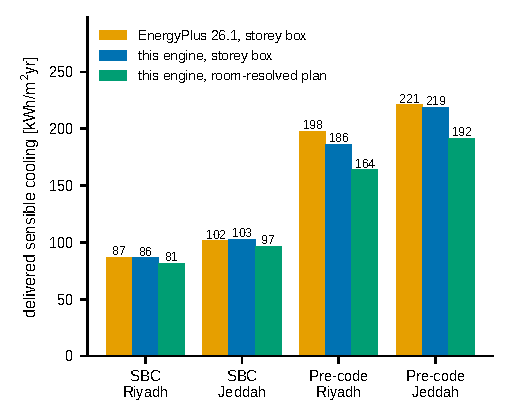
\includegraphics[width=\columnwidth]{fig_epcompare}
\caption{Like-for-like comparison with EnergyPlus~26.1: delivered sensible cooling under ideal control at the reference setpoints. On the same storey-box geometry the two programs agree within a few per cent; the room-resolved plan delivers less, because its passive rooms float above the setpoint.}
\label{fig:epcompare}
\end{figure}

\paragraph{Response to setbacks.} The scheduling result rests on how much extra heat a colder room admits. The third test therefore applies the $2\,$K pre-peak and night setbacks of the thermostat lattice to the storey box in both programs, under ideal control and with the seasonal changeover of the model (Table~\ref{tab:setback}). Both find that every setback removes more heat than holding the reference setpoint, EnergyPlus by $1.2$--$5.0$\% and the engine by $1.5$--$7.0$\%. The engine thus overstates this extra heat; EnergyPlus finds $64$--$96$\% of it. Section~\ref{sec:resched} tests whether this could change the sign of the scheduling result.

\begin{table}[t]
\centering\footnotesize\setlength{\tabcolsep}{3pt}
\caption{Response to setbacks on the storey box (ideal control): extra sensible cooling delivered by a $2\,$K setback relative to the reference setpoint [\%]. E+: EnergyPlus~26.1; this: the engine of the model.}
\label{tab:setback}
\begin{tabularx}{\linewidth}{l l C C C C}
\toprule
 & & \multicolumn{2}{c}{Pre-peak, $2\,$K} & \multicolumn{2}{c}{Night, $2\,$K} \\
\cmidrule(lr){3-4}\cmidrule(lr){5-6}
Envelope & City & E+ & this & E+ & this \\
\midrule
SBC & Riyadh & $+1.2$ & $+1.5$ & $+3.3$ & $+4.4$ \\
SBC & Jeddah & $+1.9$ & $+2.2$ & $+5.0$ & $+6.6$ \\
Pre-code & Riyadh & $+1.6$ & $+1.7$ & $+3.1$ & $+4.7$ \\
Pre-code & Jeddah & $+2.4$ & $+2.5$ & $+4.5$ & $+7.0$ \\
\bottomrule
\end{tabularx}
\end{table}

\paragraph{Stock energy use.} The stock model of \citet{stockmodel2020} puts the whole-building EUI of Saudi residential buildings at $125.6$--$182.4\,$kWh/m\textsuperscript{2}yr across the four regions, with $136.0$ for the Middle region, which contains Riyadh, and $159.6$ for the West, which contains Jeddah. For comparison, the model's HVAC energy is divided by $0.70$, a share of residential electricity for air-conditioning between the $66\%$ of the stock model and the more than $70\%$ of recent studies (Section~\ref{sec:intro}). On this basis the pre-code building, with new units at the SASO minimum and $0.4\,$ACH, uses 82 (Riyadh) and 98\,kWh/m\textsuperscript{2}yr; with the equipment and air-tightness of existing homes (Section~\ref{sec:design}) it uses 121 and 161\,kWh/m\textsuperscript{2}yr, $-11\%$ and $+1\%$ against its region's average ($-6\%$ and $+7\%$ with a share of $0.66$). This is agreement in magnitude rather than calibration, since the regional averages mix villas, apartments and traditional houses.

\subsection{Absolute and relative errors}\label{sec:errors}
Table~\ref{tab:errors} collects the error of every quantity that the study estimates against a reference; the comparison of the thermostat policies is exhaustive over the lattice, and the optimal-control programs with the indoor COP factor are approximate through their sequential-linear-programming search. None of these errors is large enough to change the ordering of the levers.

\begin{table*}[t]
\centering\footnotesize\setlength{\tabcolsep}{3pt}
\caption{Absolute and relative errors of the model's estimates against their references (pairs of values: Riyadh / Jeddah, or case 600 / 900 and 640 / 940; the BESTEST-style cases are detailed in Appendix~\ref{app:S5}).}
\label{tab:errors}
\begin{tabularx}{\linewidth}{L{4.6cm} L{4.2cm} C C}
\toprule
Quantity & Reference & Absolute error & Relative error \\
\midrule
Annual energy, 60 sampled days & full year (365 days) & $-1953$ / $+400\,$kWh & $-3.7\%$ / $+0.5\%$ \\
Annual energy, $3$-min step & $1$-min step & -- & $\le2.89\%$ \\
Passive-zone heat budget & exact balance & $\le0.6\,$W & $\le1.3\%$ \\
Annual cooling, BESTEST-style 600 / 900 & EnergyPlus & $-0.02$ / $+0.41\,$MWh & $-0.2\%$ / $+4.3\%$ \\
Annual cooling, BESTEST-style 640 / 940 & EnergyPlus & $-0.01$ / $+0.41\,$MWh & $-0.1\%$ / $+4.3\%$ \\
Extra heat removed by a $2\,$K setback, storey box & EnergyPlus & $0.1$--$2.5$ percentage points & $4$--$56$\% \\
Delivered cooling, storey box & EnergyPlus, same geometry & $-11.8$ to $+1.3$\,kWh/m\textsuperscript{2}yr & $-6.0$ to $+1.3$\% \\
Stock-equivalent EUI & regional average~\citep{stockmodel2020} & $-15$ / $+1\,$kWh/m\textsuperscript{2}yr & $-11\%$ / $+1\%$ \\
\bottomrule
\end{tabularx}
\end{table*}

\section{Results}\label{sec:results}
All results use the room-resolved model of Section~\ref{sec:model}, the TMYx weather of Riyadh and Jeddah and the per-meter volume tariff. The main case is the SBC-compliant building; the pre-code envelope (Section~\ref{sec:stock}) is reported alongside to show what code compliance is worth. Savings are bill-based and measured against the baselines of Section~\ref{sec:baselines}. Every optimum, and every saving attributed to a selected policy, compares admissible policies only (Section~\ref{sec:problem}); runs that leave the safe set are excluded and shown as ``--''. Energy is reported as the HVAC energy intensity, the electricity of the units (sensible, latent and standby) per square metre of floor. Section~\ref{sec:comfort} checks comfort and feasibility; Sections~\ref{sec:scalability}--\ref{sec:ablation} report the levers, the timing lever and the ablation; and Sections~\ref{sec:generalisation}--\ref{sec:sensitivity} test scale, stability, sensitivity and uncertainty.

\subsection{Comfort and feasibility}\label{sec:comfort}
\paragraph{Conditioned rooms.}\label{sec:comfortperf}\label{sec:minutil} At the reference policy every conditioned room of the SBC-compliant building stays at or below $24.0\,^{\circ}$C all year. The building is feasible with a wide margin: in its peak hour the busiest unit removes $19\%$ of its rated capacity in both cities, because units sized by coverage are several times larger than the loads of an insulated building, and the units are off $77\%$ (Riyadh) and $71\%$ (Jeddah) of the time. Even the pre-code building holds the ceiling with these units, its busiest unit peaking at $53$--$55$\% of its capacity, so with coverage-sized units the envelope is an energy lever; the comfort margin it buys appears when the units are sized by load (Section~\ref{sec:resinstances}). No meter reaches the $6{,}000\,$kWh tier-2 threshold: the busiest meter of the SBC-compliant building uses at most $1{,}137\,$kWh of HVAC electricity in a month, and no apartment meter of either building would exceed $4{,}579\,$kWh even if HVAC were only $66\%$ of the household's electricity~\citep{stockmodel2020}.

\paragraph{Comfort frontier.}\label{sec:frontier} Raising the cooling setpoint by the thermostat's $0.5\,$K step to $24\,^{\circ}$C lets the rooms rise $0.5\,$K above the ceiling in every cycle ($84{,}964$ and $119{,}545\,$K$\cdot$h a year), so the comfort frontier is the reference setpoint itself, the frontier that Theorem~\ref{thm:optleap} gives for a $1\,$K differential centred on the setpoint. A finer thermostat ($0.1\,$K differential, $0.05\,$K steps) at $23.5\,^{\circ}$C holds the room lower and costs more, $5.1\%$ in Riyadh and $3.0\%$ in Jeddah; its own frontier is $23.95\,^{\circ}\mathrm{C}$ in both cities, where its bill differs from that of the base thermostat by $-0.5\%$. Finer control moves the setpoint but hardly the time-mean temperature, which is what the theorem prices.

\paragraph{Passive zones.} With their doors open, the rooms without a unit stay close to their conditioned neighbours (Section~\ref{prop:passive}): in apartment 2A (Riyadh) the lobby, corridor and hall average $23.7$--$23.8\,^{\circ}\mathrm{C}$ over the year, the interior baths and the maid room $23.9$--$24.0\,^{\circ}\mathrm{C}$, and the two baths with an exterior wall $24.2\,^{\circ}\mathrm{C}$, peaking at $25.8$--$26.2\,^{\circ}\mathrm{C}$. Isolated from their neighbours (baseline B5), they would average $33.7\,^{\circ}$C instead of $24.7\,^{\circ}$C (Jeddah); the thermal shift that cools them raises the building's energy by $13.5\%$.

\paragraph{Operative temperature.}\label{sec:operative} At the reference setpoint the operative temperature of the conditioned rooms, estimated from the inner-surface temperatures of each room, peaks at $25.0$--$25.1\,^{\circ}\mathrm{C}$ (in the top-floor rooms under the roof) and exceeds $25\,^{\circ}$C in fewer than $0.05\%$ of the room-hours, inside the $23$--$27\,^{\circ}$C operative range of the ASHRAE summer comfort zone (Section~\ref{sec:comfortrange}). It lies on average $0.29$--$0.35$\,K above the air temperature, so it exceeds the $24\,^{\circ}$C air ceiling in $35.3\%$ of the room-hours in Riyadh and $46.9\%$ in Jeddah: the hard ceiling bounds the air temperature, not the operative temperature.

\subsection{Savings in the three cases}\label{sec:scalability}
\paragraph{Cases 1 and 2.}\label{sec:stepa}\label{sec:stepb} For one apartment, modelled as an intermediate apartment whose shared walls and slabs face conditioned space, the HVAC energy intensity is $23.8\,$kWh/m\textsuperscript{2}yr in Riyadh and $34.8$ in Jeddah, and the setpoint lever, from current practice to the reference setpoints, saves $12.2\%$ in Riyadh and $9.8\%$ in Jeddah (Table~\ref{tab:scopes}). Adding the neighbouring apartment and the core (Case~2) changes the representative apartment's energy by only $0.9\%$ (Riyadh) and $0.6\%$ (Jeddah), since the conditioned rooms on either side of the party wall differ by a fraction of a kelvin (Section~\ref{prop:coupling}), and moves the setpoint lever by at most $0.2$ percentage points. In both cases the best admissible thermostat policy is no pre-cooling: every pre-cooling policy of the lattice raises the bill, as Proposition~\ref{obs:precool} implies where its no-gain condition holds.

\paragraph{Case 3: the whole building.}\label{sec:stepc} The building adds the roof, the ground and the vertical coupling of four storeys. Its HVAC energy intensity is $25.1$ (Riyadh) and $37.7\,$kWh/m\textsuperscript{2}yr (Jeddah), and the setpoint lever saves $12.4\%$ in Riyadh and $10.5\%$ in Jeddah. The lever has two parts of opposite sign (percentages of the HVAC electricity at current practice, each rounded): raising the cooling setpoint from $22$ to $23.5\,^{\circ}$C saves $14.1\%$ in Riyadh and $10.5\%$ in Jeddah, about $9.4\%$ and $7.0\%$ per kelvin. Raising the heating setpoint from $20.5\,^{\circ}$C to the comfort target of $22.5\,^{\circ}$C (C5) costs $1.6\%$ in Riyadh ($6.0\%$ in the pre-code building) and nothing in Jeddah, which has no heating months. Every step of the cooling setpoint lowers the energy, and every run stays in the safe set. At the reference policy the insulated roof keeps the mean HVAC energy of a top-storey apartment within $13\%$ (Riyadh) and $9\%$ (Jeddah) of that of an apartment on an intermediate storey, whereas in the pre-code building the top apartment uses $1.5$--$1.7$ times as much; this is why the envelope saving of the whole building ($56.4\%$, $45.0\%$) exceeds that of one apartment ($50.5\%$, $38.3\%$).

\begin{table}[t]
\centering
\caption{The three cases (SBC-compliant building; pre-code value in parentheses). Intensity: HVAC energy intensity, electricity of the units per floor area [kWh/m\textsuperscript{2}yr]; the other columns are savings [\%]. Setpoint: saving of the setpoint lever, from current practice (cooling $22$, heating $20.5\,^{\circ}$C) to the reference setpoints ($23.5$ and $22.5\,^{\circ}$C). Pre-cooling: saving of the best admissible thermostat policy of the lattice. Envelope: SBC versus pre-code at the reference setpoints.}
\label{tab:scopes}
\footnotesize\setlength{\tabcolsep}{3pt}
\begin{tabularx}{\linewidth}{@{}l l C C C C@{}}
\toprule
City & Case & Intensity & Setpoint & Pre-cooling & Envelope \\
\midrule
Riyadh & 1: apartment & 23.8 (48.0) & 12.2\% & 0\% & 50.5\% \\
       & 2: floor & 23.3 (46.9) & 12.4\% & 0\% & 50.4\% \\
       & 3: building & 25.1 (57.5) & 12.4\% & 0\% & 56.4\% \\
\midrule
Jeddah & 1: apartment & 34.8 (56.4) & 9.8\% & 0\% & 38.3\% \\
       & 2: floor & 35.6 (58.4) & 9.8\% & 0\% & 38.9\% \\
       & 3: building & 37.7 (68.5) & 10.5\% & 0\% & 45.0\% \\
\bottomrule
\end{tabularx}
\end{table}

\paragraph{Savings per apartment.}\label{sec:perapt} Every apartment has its own meter, so the levers can be priced per household (Table~\ref{tab:tenants}). The setpoint lever lowers an apartment's annual HVAC bill by $152$--$190\,$SAR (US\$41--51) in Riyadh and $186$--$234\,$SAR (US\$50--62) in Jeddah, most on the ground floor, whose rooms at $22\,^{\circ}$C also draw heat from the ground. The envelope is worth far more: the same apartment in the pre-code building would cost $1{,}084$--$2{,}612\,$SAR (US\$289--697) more a year in Riyadh and $998$--$2{,}432\,$SAR (US\$266--649) more in Jeddah, most of all under the roof. Between the two mirror-image apartments of a storey, the bill at current practice differs by $2.4$--$3.2$\% of the cheaper one, the west apartment paying more in Riyadh and the east one in Jeddah, while the setpoint saving differs by at most $9\,$SAR a year. The lever percentages of the abstract and Table~\ref{tab:scopes} are for whole cases (one apartment, a floor, the building), not for each apartment.

\begin{table*}[t]
\centering\footnotesize\setlength{\tabcolsep}{4pt}
\caption{Annual HVAC bill and savings per apartment in the SBC-compliant building (Case~3; apartments numbered by storey, 1 = ground, 4 = top; A west, B east). Bill: at current practice [SAR/yr]. Setpoint: saving of the setpoint lever [SAR/yr] (\% of the bill). Envelope: extra bill of the same apartment in the pre-code building at the reference setpoints [SAR/yr] (\% of the pre-code bill). Percentages from unrounded bills.}
\label{tab:tenants}
\begin{tabularx}{\textwidth}{l C C C C C C}
\toprule
 & \multicolumn{3}{c}{Riyadh} & \multicolumn{3}{c}{Jeddah} \\
\cmidrule(lr){2-4}\cmidrule(lr){5-7}
Apartment & Bill & Setpoint & Envelope & Bill & Setpoint & Envelope \\
\midrule
1A & 1{,}433 & 190 (13.2\%) & 1{,}132 (47.7\%) & 2{,}028 & 231 (11.4\%) & 998 (35.7\%) \\
1B & 1{,}394 & 181 (13.0\%) & 1{,}084 (47.2\%) & 2{,}076 & 234 (11.3\%) & 1{,}088 (37.1\%) \\
2A & 1{,}306 & 162 (12.4\%) & 1{,}171 (50.6\%) & 1{,}869 & 189 (10.1\%) & 1{,}047 (38.4\%) \\
2B & 1{,}266 & 156 (12.3\%) & 1{,}123 (50.3\%) & 1{,}920 & 191 (9.9\%) & 1{,}135 (39.6\%) \\
3A & 1{,}307 & 159 (12.1\%) & 1{,}316 (53.4\%) & 1{,}871 & 186 (9.9\%) & 1{,}203 (41.7\%) \\
3B & 1{,}268 & 152 (12.0\%) & 1{,}263 (53.1\%) & 1{,}921 & 187 (9.7\%) & 1{,}289 (42.6\%) \\
4A & 1{,}462 & 168 (11.5\%) & 2{,}612 (66.9\%) & 2{,}044 & 212 (10.4\%) & 2{,}355 (56.2\%) \\
4B & 1{,}423 & 162 (11.4\%) & 2{,}555 (67.0\%) & 2{,}095 & 214 (10.2\%) & 2{,}432 (56.4\%) \\
\bottomrule
\end{tabularx}
\end{table*}

\paragraph{Seasons.}\label{sec:reslatent} Table~\ref{tab:summary} splits the setpoint and envelope levers by season. In summer (June--September), which carries the largest share of the energy, the setpoint lever saves $9.8$--$10.6$\% in Riyadh and $7.9$--$8.5$\% in Jeddah. In winter (December--February) it saves $11.9$--$26.6$\% (Riyadh) and $16.7$--$17.6$\% (Jeddah) of the little energy then used; in Riyadh part of that energy is heating, whose setpoint the lever raises to the comfort target. Winter is a substantial heating season only for the pre-code building in Riyadh ($11{,}116\,$kWh of heating a year, against $1{,}367\,$kWh in the SBC-compliant building). The latent load is negligible in Riyadh ($0.4\%$ of the HVAC energy) but reaches $26\%$ in Jeddah, where it dilutes the setpoint lever ($10.1\%$ for apartment 2A with it, $13.3\%$ without); the seasonal operation and the modes used are in Appendix~\ref{app:S6}.

\begin{table*}[t]
\centering\footnotesize\setlength{\tabcolsep}{3pt}
\caption{Savings of the setpoint and envelope levers by case, city and season (SBC-compliant building; \% of the HVAC energy of the case in that season; annual savings in Table~\ref{tab:scopes}). Summer: June--September; winter: December--February. Reference: HVAC energy at the reference policy [kWh]. Under the tier-1 volume tariff the bill saving equals the energy saving.}
\label{tab:summary}
\begin{tabularx}{\linewidth}{l l *{7}{C}}
\toprule
 & & Annual & \multicolumn{3}{c}{Summer} & \multicolumn{3}{c}{Winter} \\
\cmidrule(lr){3-3}\cmidrule(lr){4-6}\cmidrule(lr){7-9}
City & Case & Reference & Setpoint & Envelope & Reference & Setpoint & Envelope & Reference \\
\midrule
Riyadh & 1 & 5{,}484 & 9.8\% & 49.2\% & 3{,}313 & 26.6\% & 77.4\% & 222 \\
       & 2 & 11{,}711 & 10.0\% & 48.9\% & 7{,}126 & 25.8\% & 78.5\% & 459 \\
       & 3 & 50{,}512 & 10.6\% & 54.1\% & 31{,}239 & 11.9\% & 82.8\% & 1{,}971 \\
\midrule
Jeddah & 1 & 8{,}041 & 7.9\% & 40.0\% & 3{,}758 & 16.7\% & 33.6\% & 1{,}011 \\
       & 2 & 17{,}945 & 7.9\% & 40.1\% & 8{,}352 & 16.7\% & 36.5\% & 2{,}268 \\
       & 3 & 75{,}912 & 8.5\% & 46.3\% & 35{,}610 & 17.6\% & 41.1\% & 9{,}450 \\
\bottomrule
\end{tabularx}
\end{table*}

\subsection{The timing lever}\label{sec:resched}
\paragraph{Thermostat pre-cooling.} None of the pre-cooling settings of the lattice saves anything in any case, city or envelope (Table~\ref{tab:scopes}). Over all $365$ days, on which all of them stay within the safe set in the SBC-compliant building, every one of them raises the bill, by at least $0.52\%$, and on the sampled days the shallowest step, a $0.5\,$K pre-peak pre-cool, costs $0.51\%$ in Riyadh and $0.74\%$ in Jeddah. At a depth of $2\,$K, night pre-cooling costs $4.6\%$ in Riyadh and $5.3\%$ in Jeddah and pre-peak pre-cooling $3.4\%$ in Riyadh and $4.3\%$ in Jeddah. Table~\ref{tab:precooldecomp} splits each feature into aggregate counterparts of the two terms of Proposition~\ref{obs:precool}: every depth run ($0.5$--$2\,$K, step and ramped setbacks, default controller and low mode only) raises the heat removed by $0.12$--$8.67$\% because colder rooms admit more heat, while the mean COP rises slightly at night and falls or stays level before the peak: the heat added outweighs the COP gained. Stress tests (Appendix~\ref{app:S6}) cover inverter units held in their lowest mode, ramped and dawn setbacks, the extra heat scaled to what EnergyPlus finds, pre-cooling of the top floor or the west rooms alone, and a $1$-minute controller with minimum on- and off-times and a cycling loss charged per start (inadmissible in Riyadh, where it is excluded). None of the admissible ones saves, and, scaled to EnergyPlus's extra heat, a $2\,$K pre-peak pre-cool still costs $2.9$--$3.8$\%. Apart from the variant with one node per zone and a COP independent of the indoor air, which changes two assumptions at once ($0.08\%$; Section~\ref{sec:sensitivity}), only with every choice most favourable to pre-cooling combined (one node per zone, a COP independent of the indoor air, inverter units held in their lowest mode and no cycling loss) does the best policy save, at most $0.77\%$. Because every unit pre-cools at the same time, a $2\,$K pre-peak pre-cool also raises the building's largest hourly electrical demand, from $21.4$ to $34.1\,$kW in Riyadh and from $22.0$ to $35.3\,$kW in Jeddah.

\begin{table}[t]
\centering\footnotesize\setlength{\tabcolsep}{3pt}
\caption{Why thermostat pre-cooling does not pay (SBC-compliant building, Case~3, volume tariff): change in the annual bill, in the heat removed and in the mean cooling COP when each feature is switched on alone, relative to no scheduling. Default: the controller of Section~\ref{sec:controller}; low only: inverter units held in their lowest mode. The heat removed and the mean COP are the aggregate counterparts of the two terms of Proposition~\ref{obs:precool}, not its incremental quantities. The ramped setbacks are in the repository. Every row is admissible: it stays within the safe set (constraints (C2) and (C3)).}
\label{tab:precooldecomp}
\begin{tabularx}{\linewidth}{@{}l C C C c@{}}
\toprule
 & \multicolumn{1}{c}{Default} & \multicolumn{3}{c}{Low mode only} \\
\cmidrule(lr){2-2}\cmidrule(lr){3-5}
Feature & Bill & Bill & Heat removed & Mean COP \\
\midrule
\multicolumn{5}{@{}l}{\emph{Riyadh}} \\
Pre-peak, $0.5\,$K & $+0.51\%$ & $+0.48\%$ & $+0.40\%$ & 3.44$\to$3.44 \\
Pre-peak, $2\,$K & $+3.40\%$ & $+1.95\%$ & $+1.96\%$ & 3.44$\to$3.44 \\
Night, $0.5\,$K & $+0.95\%$ & $+0.97\%$ & $+1.32\%$ & 3.44$\to$3.45 \\
Night, $2\,$K & $+4.57\%$ & $+3.88\%$ & $+5.71\%$ & 3.44$\to$3.49 \\
\midrule
\multicolumn{5}{@{}l}{\emph{Jeddah}} \\
Pre-peak, $0.5\,$K & $+0.74\%$ & $+0.65\%$ & $+0.61\%$ & 3.63$\to$3.62 \\
Pre-peak, $2\,$K & $+4.30\%$ & $+2.84\%$ & $+3.05\%$ & 3.63$\to$3.60 \\
Night, $0.5\,$K & $+1.15\%$ & $+1.11\%$ & $+1.92\%$ & 3.63$\to$3.64 \\
Night, $2\,$K & $+5.27\%$ & $+4.72\%$ & $+8.67\%$ & 3.63$\to$3.70 \\
\bottomrule
\end{tabularx}
\end{table}

\begin{runexc}
Apartment 2A of the SBC-compliant building in Riyadh (Case~3) pays $1{,}144\,$SAR (US\$305) a year at the reference policy. A thermostat that pre-cools by $2\,$K before the afternoon adds about $39\,$SAR a year to that bill and nothing to comfort: under the Saudi tariff the right setting is to switch night and pre-peak pre-cooling off.
\end{runexc}

\paragraph{Perfect-foresight benchmark.}\label{sec:lowerbound} With perfect knowledge of the weather, the linear program of Section~\ref{sec:lpbench} schedules the idealised units of Cases~1 and~2, of the top floor under the roof and, for the bound only, of the whole building (Case~3). It compares the result with holding the ceiling with the same units (Table~\ref{tab:lowerbound} shows selected design days; all are in the repository, Appendix~\ref{app:S2}, and the ranges below are over all of them). With a COP that depends on the outdoor air only ($\gamma=0$), its saving is an upper bound on what any periodic schedule of the idealised model could save: at most $1.9\%$ of the sensible cooling electricity on a design day with the rooms kept in the comfort band and $3.6\%$ down to the $20\,^{\circ}$C floor of the safe set. Weighted over the May--September mean days of Case~1, the daily bounds average $0.58$--$1.07$\% within the band and $1.03$--$2.07$\% down to $20\,^{\circ}$C, a weighted mean that is not itself a bound for the season. Under the roof the bound is smaller than on the typical floor: $0.75\%$ in Riyadh and $0.35\%$ in Jeddah on the mean July day within the band, against $1.39\%$ in Riyadh and $0.86\%$ in Jeddah for the typical floor. For the whole building it is $0.13$--$1.34$\% within the band and $0.22$--$2.50$\% down to $20\,^{\circ}$C on the design days of Case~2, below the typical floor on every day.

With the engine's indoor COP factor ($\gamma=0.02$) the program is not linear. The achievable saving, that of the best valid schedule found by the search of Section~\ref{sec:lpbench}, is $0.00$--$0.63$\% within the band and $0.00$--$0.67$\% down to $20\,^{\circ}$C on a design day, and $0.23\%$ in Riyadh and $0.06\%$ in Jeddah within the band over the season in Case~1.

With July treated as one $31$-day horizon (Case~1), which lets heat be stored across days, the program achieves $0.33\%$ in Riyadh and $0.23\%$ in Jeddah, against $0.28\%$ in Riyadh and $0.10\%$ in Jeddah for the mean July day, with a bound of $1.31\%$ in Riyadh and $0.96\%$ in Jeddah.

The program saves in the way Proposition~\ref{obs:precool} allows: it pulls the rooms down around dawn, when the outdoor air is coolest and the COP highest (the rooms are coldest at 06:00 in the Riyadh July profile), never uses more than the lowest mode, and lets the rooms rise to the ceiling through the hottest hours. Its linearisation and its search are checked in Appendix~\ref{app:S2}. The benchmark's continuous low-mode modulation without cycling losses is part of what it measures: a dawn setback fixed in advance, which imitates its timing on a simulated thermostat, raises the bill of the whole building (Case~3) by $0.99$--$1.80$\% (Appendix~\ref{app:S6}).

\begin{table*}[t]
\centering\footnotesize\setlength{\tabcolsep}{2.5pt}
\caption{Perfect-foresight benchmark (SBC-compliant building): saving [\%] of the sensible cooling electricity that an ideal schedule achieves over holding the $24\,^{\circ}$C ceiling with the same idealised units, with the rooms pre-cooled at most to the band floor ($22\,^{\circ}$C) or to the floor of the safe set ($20\,^{\circ}$C), with a COP that depends on the outdoor air only ($\gamma=0$) or the COP of the engine ($\gamma=0.02$, falling by $2\%$/K of indoor air below $27\,^{\circ}$C). The $\gamma=0$ columns are upper bounds on the saving of any periodic schedule of the idealised model on that horizon; the $\gamma=0.02$ columns are achievable savings, those of the best valid schedule found (Section~\ref{sec:lpbench}). Hold: electricity of the reference at $\gamma=0.02$ [kWh/day]. Season: May--September mean days weighted by the reference energy of their month (Case~1), a weighted mean of the daily values and not itself a bound for the season; July, 31 days: the whole month as one horizon (Case~1, band floor only). Case~3: the bound only; the search at $\gamma=0.02$ is not run. Selected design days; every design day is in the repository (Appendix~\ref{app:S2}).}
\label{tab:lowerbound}
\begin{tabularx}{\linewidth}{l l C C C C C C C C C C}
\toprule
 & & \multicolumn{5}{c}{Riyadh} & \multicolumn{5}{c}{Jeddah} \\
\cmidrule(lr){3-7}\cmidrule(lr){8-12}
 & & & \multicolumn{2}{c}{$\gamma=0.02$ (achievable)} & \multicolumn{2}{c}{$\gamma=0$ (bound)} & & \multicolumn{2}{c}{$\gamma=0.02$ (achievable)} & \multicolumn{2}{c}{$\gamma=0$ (bound)} \\
\cmidrule(lr){4-5}\cmidrule(lr){6-7}\cmidrule(lr){9-10}\cmidrule(lr){11-12}
Case & Day & Hold & $22\,^{\circ}$C & $20\,^{\circ}$C & $22\,^{\circ}$C & $20\,^{\circ}$C & Hold & $22\,^{\circ}$C & $20\,^{\circ}$C & $22\,^{\circ}$C & $20\,^{\circ}$C \\
\midrule
1: apartment & Jul, mean day & 22.3 & 0.28 & 0.28 & 1.26 & 2.41 & 16.8 & 0.10 & 0.10 & 0.78 & 1.43 \\
 & Jul, hottest day & 25.4 & 0.46 & 0.47 & 1.50 & 2.86 & 19.3 & 0.54 & 0.54 & 1.79 & 3.34 \\
& Season & -- & 0.23 & 0.23 & 1.07 & 2.07 & -- & 0.06 & 0.06 & 0.58 & 1.03 \\
& Jul, 31 days & 22.3 & 0.33 & -- & 1.31 & -- & 16.9 & 0.23 & -- & 0.96 & -- \\
\midrule
2: floor & Jul, mean day & 46.6 & 0.35 & 0.35 & 1.39 & 2.65 & 35.9 & 0.13 & 0.13 & 0.86 & 1.58 \\
 & Jul, hottest day & 53.8 & 0.54 & 0.56 & 1.63 & 3.09 & 41.6 & 0.63 & 0.67 & 1.92 & 3.57 \\
Top floor & Jul, mean day & 55.8 & 0.12 & 0.12 & 0.75 & 1.42 & 43.5 & 0.02 & 0.02 & 0.35 & 0.63 \\
 & Jul, hottest day & 64.5 & 0.19 & 0.19 & 0.96 & 1.82 & 50.1 & 0.25 & 0.25 & 1.08 & 2.02 \\
3: building & Jul, mean day & 204.8 & -- & -- & 0.94 & 1.78 & 157.3 & -- & -- & 0.50 & 0.91 \\
 & Jul, hottest day & 235.6 & -- & -- & 1.16 & 2.21 & 181.1 & -- & -- & 1.34 & 2.50 \\
\bottomrule
\end{tabularx}
\end{table*}

\subsection{Ablation study}\label{sec:ablation}
The selected policy $\theta^\ast$ has four components: the frontier cooling setpoint (the $23.5\,^{\circ}$C reference; the heating setpoint is fixed by (C5)), no pre-cooling, the controller's mode selection (lowest mode first, escalating when a room lags) and the SBC envelope. Table~\ref{tab:ablation} changes one of them at a time (Case~3; the simulation is deterministic, so each variant is a single annual run). The envelope matters most: the pre-code envelope raises the bill by $129.5\%$ in Riyadh and $81.8\%$ in Jeddah. Lowering the cooling setpoint to $22\,^{\circ}$C, with heating then capped at $21\,^{\circ}$C, costs $14.5\%$ in Riyadh and $11.7\%$ in Jeddah, which differs from the setpoint lever of Table~\ref{tab:scopes} because that lever starts from heating at $20.5\,^{\circ}$C and is expressed relative to current practice. Running every inverter unit in its highest mode costs $22.4\%$ in Riyadh and $17.3\%$ in Jeddah; this largely reproduces the assumed ratio of mode efficiencies (Theorem~\ref{thm:optleap}). The pre-cooling rows carry the penalties of Section~\ref{sec:resched}. The only variant cheaper than $\theta^\ast$ holds the inverter units in their lowest mode, a controller variant of Section~\ref{sec:sensitivity}: it changes the bill by $-0.31\%$ in Riyadh and $-0.03\%$ in Jeddah and keeps every room in the safe set. The mode rule is a property of the controller, not of the policy $\theta$ that a household sets, so the escalation of $\theta^\ast$ costs at most this margin.

\begin{table}[t]
\centering\footnotesize\setlength{\tabcolsep}{3pt}
\caption{Ablation of the selected policy $\theta^\ast$ (whole building, Case~3, volume tariff). Each variant changes one component and keeps the others, including the heating setpoint (which Algorithm~\ref{alg:eval} caps at $1\,$K below the cooling setpoint, so the current-practice row heats to $21\,^{\circ}$C). Bill: annual HVAC bill (SAR); $\Delta$: its change relative to $\theta^\ast$ [\%]. All variants keep every conditioned room within the safe set (zero excursion above $24\,^{\circ}$C and below $20\,^{\circ}$C) and are therefore admissible. Lowest bill in bold.}
\label{tab:ablation}
\begin{tabularx}{\linewidth}{@{}X r r r r@{}}
\toprule
 & \multicolumn{2}{c}{Riyadh} & \multicolumn{2}{c}{Jeddah} \\
\cmidrule(lr){2-3}\cmidrule(l){4-5}
Variant (changed component) & Bill & $\Delta$ & Bill & $\Delta$ \\
\midrule
Selected policy $\theta^\ast$ (SBC) & 10{,}456 & -- & 15{,}714 & -- \\
\midrule
Current-practice cooling ($23.5\to22\,^{\circ}$C; heating $21\,^{\circ}$C) & 11{,}968 & $+14.5$ & 17{,}551 & $+11.7$ \\
Inverter units in lowest mode (controller) & \textbf{10{,}424} & $-0.31$ & \textbf{15{,}709} & $-0.03$ \\
Highest mode (instead of the lowest) & 12{,}801 & $+22.4$ & 18{,}440 & $+17.3$ \\
Pre-code envelope (instead of SBC) & 23{,}994 & $+129.5$ & 28{,}566 & $+81.8$ \\
Night pre-cooling ($2\,$K) & 10{,}934 & $+4.6$ & 16{,}542 & $+5.3$ \\
Pre-peak pre-cooling ($2\,$K) & 10{,}811 & $+3.4$ & 16{,}390 & $+4.3$ \\
\bottomrule
\end{tabularx}
\end{table}

\paragraph{Factorial decomposition.}\label{sec:factorial} The one-at-a-time levers are measured against different baselines. A full $2^4$ factorial of four levers (envelope, the 3-ton units as inverter units, the setpoints of current practice or of the reference, and a $2\,$K pre-peak pre-cool or none; Case~3, all $16$ combinations admissible) puts them on one base. Going from the pre-code building with catalogue units, current-practice setpoints and pre-peak pre-cooling to the SBC-compliant building with inverter units, the reference setpoints and no pre-cooling lowers the building's annual HVAC bill from $26{,}788$ to $8{,}889\,$SAR (US\$7{,}143 to US\$2{,}370) in Riyadh and from $33{,}616$ to $13{,}924\,$SAR (US\$8{,}964 to US\$3{,}713) in Jeddah, savings of $66.8\%$ and $58.6\%$. Table~\ref{tab:factorial} attributes this saving to the levers by their Shapley values, the average of each lever's marginal saving over every order in which the levers can be applied. The envelope takes $74.6\%$ of it in Riyadh and $68.6\%$ in Jeddah, and dropping pre-cooling takes the least, $2.3\%$ in Riyadh and $3.8\%$ in Jeddah. The levers are sub-additive: each saves less once another has lowered the load, most for the envelope with the equipment in Riyadh and the envelope with the setpoints in Jeddah (an interaction of up to $7.0\%$ of the starting bill), while pre-cooling interacts with the other levers by at most $0.9\%$. In both cities the envelope comes first and timing last; the equipment saves more than the setpoints in Riyadh, and the two, close to each other, swap places in SAR in Jeddah, as in the one-at-a-time results. The Shapley value of the timing lever is the avoided penalty of its start level, the $2\,$K pre-peak pre-cool: because no tested pre-cool saves, pre-cooling only costs and timing ranks last; its share would grow with a deeper start level and vanish without one. The ranking also compares steps chosen for the study (the code envelope, a $1.5\,$K setpoint step, one unit type), so it orders these steps, not the levers in general; the mode lever is not part of the factorial, since the controller sets the mode.

\begin{table}[t]
\centering\footnotesize\setlength{\tabcolsep}{3pt}
\caption{Factorial ($2^4$) decomposition of the bill saving (Case~3). Levers, from start to end state: pre-code $\to$ SBC envelope; fixed-speed $\to$ inverter 3-ton units; setpoints $22/20.5\to23.5/22.5\,^{\circ}$C; $2\,$K pre-peak pre-cool $\to$ none. Shapley value: each lever's marginal saving averaged over all orders (SAR/yr and share of the total); main effect: mean saving of the lever over the eight combinations of the others (\% of the bill without it). Values are rounded individually, so the rows may not add exactly to the total.}
\label{tab:factorial}
\begin{tabular*}{\linewidth}{@{\extracolsep{\fill}}l r r r r r r@{}}
\toprule
 & \multicolumn{3}{c}{Riyadh} & \multicolumn{3}{c}{Jeddah} \\
\cmidrule(lr){2-4}\cmidrule(lr){5-7}
Lever & SAR & Share & Main & SAR & Share & Main \\
\midrule
Envelope & 13{,}346 & $74.6\%$ & $56.0\%$ & 13{,}503 & $68.6\%$ & $45.7\%$ \\
Inverter 3-ton units & 2{,}395 & $13.4\%$ & $13.5\%$ & 2{,}667 & $13.5\%$ & $11.1\%$ \\
Setpoints & 1{,}742 & $9.7\%$ & $10.2\%$ & 2{,}774 & $14.1\%$ & $11.0\%$ \\
No pre-cooling & 416 & $2.3\%$ & $2.6\%$ & 747 & $3.8\%$ & $3.4\%$ \\
\midrule
Total & 17{,}899 & $100\%$ & & 19{,}692 & $100\%$ & \\
\bottomrule
\end{tabular*}
\end{table}

\subsection{Generalisation: scale and test instances}\label{sec:generalisation}
\paragraph{Scale and saturation.}\label{sec:threshold} Across the three cases the model grows from $16$ to $33$ to $132$ zones and from $7$ to $15$ to $60$ units, yet the optimum stays at no pre-cooling in every case, city and envelope: scale changes the load on each unit but not the value of re-timing, and how close the units come to their capacity depends on the envelope and on how they are sized (Table~\ref{tab:instances}).

\paragraph{Normal and hard instances.}\label{sec:resinstances} All eight instances with the catalogue units are normal: even in the heat-wave year, $3\,$K hotter in every hour, the peak load ratio stays at or below $0.26$ in the SBC-compliant building and $0.62$ in the pre-code building, because units sized by coverage leave a wide margin even for the uninsulated envelope. Hard instances arise when the units are sized tightly, each to $1.15$ times its room's largest hourly load, after derating, rounded up to a multiple of $0.25\,$ton (at least $0.75\,$ton). All four such instances are hard. Their peak load ratio rises to $0.57$--$0.79$, so they satisfy the feasibility condition~\eqref{eq:feasible} on hourly loads, yet the rooms exceed the ceiling by $18$--$81$\,K$\cdot$h a year. These excursions do not reflect a shortage of hourly capacity. Starting each unit at full capacity leaves them unchanged, so they do not arise at start-up: they arise while a running unit escalates from a lower mode, with the switch-on point at the ceiling itself (Appendix~\ref{app:S6}). At the reference setpoints no lattice setting, with or without pre-cooling, is admissible in any of the four. A lower cooling setpoint, which moves the switch-on point below the ceiling, restores admissibility. The highest admissible setpoint is $23\,^{\circ}$C in all of them; there the tightly sized units still save $10.2$--$16.7$\% against the catalogue units at the reference policy, so for these units, with no tolerance on the safe set, the optimum moves to a lower setpoint rather than to another lattice setting.

\paragraph{Tolerance of the safe set.}\label{sec:tolerance} Admissibility requires zero excursion, a strict rule. Allowing a tolerance of $0.05$, $0.1$ or $0.2\,$K on both bounds leaves the result unchanged with the catalogue units: in the four instances of the TMYx year the reference policy stays admissible and no pre-cooling stays the best policy; only the number of admissible lattice policies of the pre-code building in Jeddah grows, from $36$ to $41$ at $0.1\,$K and $42$ at $0.2\,$K. The tightly sized units exceed the ceiling by at most $0.15$--$0.19$\,K at the reference policy, so of the tolerances tested only $0.2\,$K makes their reference admissible, where no pre-cooling is again the best policy. At $0.1\,$K or less the reference stays inadmissible, and only pre-cooling settings stay within the bounds (at $0.1\,$K, 7 and 30 of the $49$ in the SBC-compliant building in Riyadh and Jeddah, and none and 7 in the pre-code building), so the cheapest admissible setting is then a pre-cooling one.

\begin{table*}[t]
\centering\footnotesize\setlength{\tabcolsep}{3pt}
\caption{Normal and hard test instances (Case~3, the whole building). Catalogue: the eight instances with the catalogue units (two envelopes, two cities, TMYx and TMYx $+3\,$K weather) in one row, with ranges over them; every instance is in the repository (Appendix~\ref{app:S6}). Units: catalogue (sized by coverage) or each sized to its room's own peak hourly load with a $15\%$ margin. Peak load ratio: largest hourly sensible load of any unit over its rated capacity; Exc.: excursion of the reference policy above $24\,^{\circ}$C and below $20\,^{\circ}$C; best policy: the cheapest admissible thermostat policy, night/pre-peak depth (none: no pre-cooling; --: no lattice setting at the reference setpoints is admissible; in brackets, the highest admissible cooling setpoint without pre-cooling, where one exists); admissible policies: number of the $49$ lattice policies that keep every conditioned room within the safe set on the sampled days (the others are excluded). No unit reaches a load ratio of $0.85$.}
\label{tab:instances}
\begin{tabularx}{\linewidth}{l l l l c c c c C}
\toprule
Envelope & City & Units & Weather & Class & Peak load ratio & Exc.\ above/below [K$\cdot$h] & Best policy & Admissible policies \\
\midrule
SBC, pre-code & both & catalogue & both & normal & $0.19$--$0.62$ & 0/0 & none & $30$--$49$ of $49$ \\
\midrule
SBC & Riyadh & by load & TMYx & hard & 0.58 & 69/0 & -- ($23\,^{\circ}$C) & $0$ of $49$ \\
SBC & Jeddah & by load & TMYx & hard & 0.57 & 18/0 & -- ($23\,^{\circ}$C) & $0$ of $49$ \\
Pre-code & Riyadh & by load & TMYx & hard & 0.79 & 81/0 & -- ($23\,^{\circ}$C) & $0$ of $49$ \\
Pre-code & Jeddah & by load & TMYx & hard & 0.75 & 29/0 & -- ($23\,^{\circ}$C) & $0$ of $49$ \\
\bottomrule
\end{tabularx}
\end{table*}

\subsection{Thermostat comparison: full-year re-evaluation and calculation time}\label{sec:optimisation}
\paragraph{Selection and full-year re-evaluation.}\label{sec:stability}\label{sec:trainevalres} The comparison is exhaustive over the $49$ realisable thermostat policies, and its best policy, no pre-cooling, is the same in all four envelope--climate configurations and in every case and test instance with an admissible reference policy. Selected on the $60$ sampled days and re-evaluated on all $365$ days of the year, which include them (Section~\ref{sec:gasetup}), the optimum for the SBC-compliant building is unchanged in both cities, and the policies keep almost the same cost ranking (Spearman rank correlation $0.999$ in both cities). The sampled-year estimate of the building's annual HVAC energy at the reference policy differs from the full-year value by $-3.7\%$ (Riyadh) and $+0.5\%$ (Jeddah), and the relative cost of every pre-cooling policy by at most $0.56$ percentage points. Unless labelled as full-year, absolute energies and bills are sampled-year values.
 Admissibility, checked on the sampled days, also holds on all $365$ days for every run the results rely on: the $16$ runs of the factorial, the units sized by load at the selected margin and the dawn setback stay within the safe set in both cities. In the pre-code building 29 of the 49 lattice policies stay within the safe set over the full year in each city, fewer than on the sampled days (Table~\ref{tab:instances}); the cheapest of them is still no pre-cooling, and every other one costs more, at least $0.51\%$ in Riyadh and $0.74\%$ in Jeddah.

\paragraph{Calculation time.}\label{sec:time} On a two-core virtual machine one annual evaluation of the whole building ($132$ zones with two nodes each, $120$ open doors, $28{,}800$ steps) takes $13.4\,$s for one policy and $52.5\,$s for all $49$ policies of the lattice together. The optimal-control program for one day has $5{,}088$ variables in Case~1 and $10{,}656$ in Case~2; its bound ($\gamma=0$, one solve) takes $1.3$ and $18.4\,$s, and the search for the indoor COP factor ($19$ solves) $21.2$ and $284.3\,$s, so its time grows about 13-fold for twice the zones, while the simulation time hardly grows. The bound of the whole building, with Clarabel, takes $233.8\,$s. Selecting the modes of all $60$ units at one control step takes $8.4\,\mu$s, and a single unit's thermostat logic is trivial for ordinary hardware. Every measured time, for the three cases, is in the repository (\path{results/csv/repository/calculation_time.csv}).

\subsection{Sensitivity analysis}\label{sec:sensitivity}
The sensitivity analysis varies, one at a time, the assumed inputs and model choices: the zone model, the controller and COP model, the equipment, the envelope and air, and the weather (37 variants of the SBC-compliant building; Table~\ref{tab:robust} shows the decisive ones, and the full table is in the repository, Appendix~\ref{app:S6}). In 35 of the 36 admissible variants the best thermostat pre-cool saves nothing, and a $2\,$K pre-peak pre-cool costs $2.0$--$6.7$\%; the only exception, a one-node zone whose COP does not depend on the room temperature (two changes at once), saves at most $0.08\%$, and its $2\,$K pre-peak pre-cool still costs $1.8\%$. The variant sized by load with a $15\%$ margin is inadmissible: the reference policy already lets a room pass the ceiling, by $69\,$K$\cdot$h a year in Riyadh and $18\,$K$\cdot$h a year in Jeddah, so no lever or cost is reported for it (``excluded'' in Table~\ref{tab:robust}). The setpoint lever stays between $8.0$ and $17.0\%$.

\paragraph{Equipment.} In the SBC-compliant building the installed equipment matters more than its operation. Without cycling losses the building would use $15.2\%$ less energy in Riyadh and $11.8\%$ less in Jeddah, and replacing the twelve fixed-speed 3-ton units by inverter units of the same size would save $15.0\%$ in Riyadh and $11.4\%$ in Jeddah; these guest-room and stair units, the most oversized, use $39$--$40$\% of the units' electricity for $33\%$ of the conditioned floor area. Units sized by load keep every room within the safe set only with a margin of $2.5$ times each room's peak hourly load (the smallest sufficient margin lies between $2$ and $2.5$; Appendix~\ref{app:S6}). Against the catalogue's $124$ tons, such units would save $16.5\%$ in Riyadh and $11.2\%$ in Jeddah as inverter units throughout, and $2.1\%$ in Riyadh and $0.2\%$ in Jeddah with the fixed-speed zones keeping fixed-speed units, which isolates the effect of size. An indoor fan of $30\,$W that runs whenever the compressor is off in the cooling months, as many wall-mounted units do by default, adds $11.8\%$ in Riyadh and $14.7\%$ in Jeddah, comparable to the setpoint lever, although whether the catalogue units do so was not established. None of these changes the ordering of the operational levers or makes pre-cooling pay.

\paragraph{Controller and COP model.} With escalation at $0.2$/$0.6\,$K, a $2\,$K pre-peak pre-cool costs $3.1\%$ in Riyadh and $4.4\%$ in Jeddah; with escalation at $0.8$/$2.0\,$K it costs $2.3\%$ in Riyadh and $3.2\%$ in Jeddah, and with the inverter units held in their lowest mode $2.0\%$ in Riyadh and $2.8\%$ in Jeddah. Without the indoor-temperature factor of the COP the setpoint lever falls to $9.5\%$ in Riyadh and $8.1\%$ in Jeddah and the $2\,$K pre-peak cost to $2.2\%$ in Riyadh and $3.0\%$ in Jeddah; with an indoor slope of $3\%$/K the lever rises to $14.0\%$ in Riyadh and $11.8\%$ in Jeddah and the penalty to $4.1\%$ in Riyadh and $5.1\%$ in Jeddah. The cycle length, set by the time step, moves the absolute bill but not the sign of pre-cooling (Appendix~\ref{app:S6}).

\paragraph{Zone model, envelope and weather.} With one node per zone, so that a pull-down stores coolth in the whole mass at once, a $2\,$K pre-peak pre-cool still costs $3.3\%$ in Riyadh and $6.7\%$ in Jeddah, because the colder room also lowers the COP. The air-node share of the capacitance ($2$ to $30\%$) and the air--structure coupling (halved or doubled) leave the best pre-cool at $0.00$\%; thermal bridges and the solar absorptance move the energy by a few per cent; infiltration between $0.2$ and $0.8\,$ACH moves Jeddah's intensity from $30.4$ to $52.4\,$kWh/m\textsuperscript{2}yr through the latent load; and a $30\%$ wider daily swing, alone or in a heat wave, leaves the scheduling result unchanged. A room capacitance of $144$ to $450\,$kJ/(m$^2$K) leaves the best pre-cool at $0$\% (Jeddah), and an imposed day--night COP swing makes pre-cooling pay only far beyond the physical range (in Jeddah only once the COP at $22\,^{\circ}$C is $4.0$ times that at $40\,^{\circ}$C, and in Riyadh not at all up to a ratio of $6.7$, against a ratio of $1.5$ for the model's curve).

\begin{table*}[t]
\centering\footnotesize\setlength{\tabcolsep}{2.5pt}
\caption{Sensitivity analysis (SBC-compliant building, Case~3): HVAC energy intensity [kWh/m\textsuperscript{2}yr], setpoint lever, saving of the best thermostat pre-cool ($0.5$--$2\,$K in either window; positive: saves), and the change in cost of a $2\,$K pre-peak pre-cool (positive: costs). $C_d$: cycling degradation coefficient; sized by load: at $2.5$ times the peak hourly load, the first tested margin that keeps every room within the safe set, unless stated; excluded: inadmissible, because the reference policy lets a room leave the safe set by the annual excursion shown; nothing else of the run is reported. Selected variants; all 37 are in the repository (Appendix~\ref{app:S6}).}
\label{tab:robust}
\begin{tabularx}{\linewidth}{L{4.6cm} *{8}{C}}
\toprule
 & \multicolumn{4}{c}{Riyadh} & \multicolumn{4}{c}{Jeddah} \\
\cmidrule(lr){2-5}\cmidrule(lr){6-9}
Variant & Int. & Setp. & Pre-cool & $2\,$K & Int. & Setp. & Pre-cool & $2\,$K \\
\midrule
Reference (base case) & 25.1 & 12.4\% & 0.00\% & $+3.4\%$ & 37.7 & 10.5\% & 0.00\% & $+4.3\%$ \\
\midrule
One node, COP independent of indoor air & 23.8 & 8.2\% & 0.08\% & $+1.8\%$ & 36.1 & 8.0\% & 0.00\% & $+5.0\%$ \\
Escalation at $0.2$ / $0.6\,$K & 26.0 & 12.6\% & 0.00\% & $+3.1\%$ & 38.5 & 10.8\% & 0.00\% & $+4.4\%$ \\
COP independent of indoor air & 23.6 & 9.5\% & 0.00\% & $+2.2\%$ & 36.0 & 8.1\% & 0.00\% & $+3.0\%$ \\
Indoor COP factor $3\%$/K & 25.9 & 14.0\% & 0.00\% & $+4.1\%$ & 38.6 & 11.8\% & 0.00\% & $+5.1\%$ \\
\midrule
No cycling loss ($C_d=0$) & 21.3 & 12.5\% & 0.00\% & $+4.0\%$ & 33.2 & 10.1\% & 0.00\% & $+4.8\%$ \\
3-ton units as inverter units & 21.3 & 12.4\% & 0.00\% & $+4.5\%$ & 33.4 & 10.0\% & 0.00\% & $+5.2\%$ \\
Sized by load, all inverter & 20.9 & 11.7\% & 0.00\% & $+2.9\%$ & 33.5 & 9.6\% & 0.00\% & $+3.0\%$ \\
Sized by load, fixed-speed kept & 24.5 & 11.9\% & 0.00\% & $+2.6\%$ & 37.6 & 10.1\% & 0.00\% & $+2.9\%$ \\
Sized by load with a $15\%$ margin & \multicolumn{4}{c}{excluded: $68.6\,$K$\cdot$h above} & \multicolumn{4}{c}{excluded: $17.8\,$K$\cdot$h above} \\
Indoor fan on while compressor off & 28.0 & 10.9\% & 0.00\% & $+3.3\%$ & 43.2 & 8.8\% & 0.00\% & $+4.1\%$ \\
\midrule
Infiltration $0.8\,$ACH & 31.5 & 10.0\% & 0.00\% & $+3.4\%$ & 52.4 & 10.2\% & 0.00\% & $+3.8\%$ \\
Heat wave $+3\,$K, swing $\times1.3$ & 33.4 & 12.2\% & 0.00\% & $+3.1\%$ & 46.7 & 9.7\% & 0.00\% & $+4.1\%$ \\
\bottomrule
\end{tabularx}
\end{table*}

\paragraph{Humidity.} A diagnostic humidity balance per zone (Appendix~\ref{app:S6}) tests the assumption that the indoor humidity target is met. It holds in Riyadh, where the conditioned rooms exceed $60\%$ relative humidity in $0.8\%$ of the cooling-season hours, but not in Jeddah, where the oversized units run too briefly: at a sensible heat ratio of $0.75$ the rooms exceed $60\%$ in $41\%$ of the hours, so holding the target needs dedicated dehumidification, whose electricity the latent term prices. The Jeddah results therefore price humidity but do not constrain it. The setpoint lever hardly moves this diagnostic, and pre-peak pre-cooling worsens it.

\paragraph{Cost model.}\label{sec:senscost} Under three energy-priced tariffs (a flat price of $0.18\,$SAR/kWh before VAT, the actual two tiers, and the two tiers with the threshold lowered from $6{,}000$ to $500\,$kWh a month, which the apartment meters exceed in summer), no pre-cooling remains optimal, with $0\%$ saving, as Proposition~\ref{thm:policy} implies for any tariff of energy alone once the no-gain condition of Proposition~\ref{obs:precool} holds. The stricter tier only raises the $2\,$K pre-peak cost, to $4.4\%$ in Riyadh and $5.3\%$ in Jeddah at the $500\,$kWh threshold, because part of the extra energy is billed in the higher tier.

\paragraph{Contrast: a time-of-use tariff.} To check that the null result is a property of the tariff rather than of the model, the same lattice is priced under an illustrative time-of-use tariff that charges the cooling-month energy used from 13:00 to 17:00 at $r$ times the off-peak price. The window is that of the Saudi time-of-use programme for large industrial and commercial customers, which did not include households~\citep{sec_tou2010}. At $r=1$ the result is that of the volume tariff. At $r=2$, $3$ and $5$ the best schedule pre-cools before the peak and saves $2$--$27$\% with the base-case zones ($13$--$50$\% with one node per zone, whose air holds the full capacitance). The same model that finds no value in re-timing under the Saudi tariff therefore finds it as soon as the tariff prices the hour.

\paragraph{Global uncertainty analysis.}\label{sec:uq} The one-at-a-time runs leave the joint effect of the assumed inputs open. Seventeen of them (Appendix~\ref{app:S7}) are varied together over uniform ranges by a Latin hypercube of $128$ samples per city; the per-sample results are in the repository. The reference policy is admissible in every sample; the pre-code building, which serves only as the envelope comparison, leaves the safe set in $66$--$68$ of them. As admissibility requires, those comparisons are excluded, and the envelope lever is taken over the other $60$--$62$ samples. Over all samples, including those in which the pre-code building leaves the safe set (and so holds its rooms warmer, which understates its energy and the lever), the envelope lever has a $5$--$95\%$ range of $49.0$--$59.8\%$ (median $53.6\%$) in Riyadh and $33.9$--$51.2\%$ (median $41.7\%$) in Jeddah. Over the admissible comparisons the medians are $54.3\%$ and $42.4\%$, so the exclusion moves the median by at most $0.7$ percentage points. Table~\ref{tab:uq} gives the median and the $5$--$95\%$ range of each result. None of the pre-cooling settings tested in each sample ($0.5$--$2\,$K, night or pre-peak) saves in any of the $256$ samples, and a $2\,$K pre-peak pre-cool costs in every sample. The ordering (envelope, then setpoints, then timing) holds in every sample in which all the compared runs are admissible, and in all $256$ samples if the inadmissible pre-code comparisons are included. With none of $128$ samples per city saving, the share of the sampled input space in which a tested pre-cooling setting saves is below $3/128\approx2.3\%$ per city at $95\%$ confidence (rule of three; approximate here, since a Latin hypercube is not a simple random sample). The analysis varies assumed inputs only, not the ceiling, occupancy, tariff, sizing, controller logic or policy class. The setpoint lever depends most on the indoor COP slope $\gamma$ and the infiltration, the cost of pre-peak pre-cooling on the indoor COP slope $\gamma$ and the air-node share of capacitance (partial rank correlations, Riyadh; both cities in Appendix~\ref{app:S7}).

\begin{table}[t]
\centering\footnotesize\setlength{\tabcolsep}{1.5pt}
\caption{Global uncertainty analysis (SBC-compliant building, Case~3, $128$ Latin-hypercube samples of $17$ assumed inputs per city): median and $5$--$95\%$ range of each result [\%], over the samples in which both compared runs are admissible (envelope: $62$ and $60$ samples in Riyadh and Jeddah; all others: $128$). Levers are savings; pre-cooling rows are the saving of the best admissible pre-cool and the cost of a $2\,$K pre-cool. Ranges of the inputs and the partial rank correlations: Appendix~\ref{app:S7}.}
\label{tab:uq}
\begin{tabular*}{\linewidth}{@{\extracolsep{\fill}}l r r r r@{}}
\toprule
 & \multicolumn{2}{c}{Riyadh} & \multicolumn{2}{c}{Jeddah} \\
\cmidrule(lr){2-3}\cmidrule(lr){4-5}
Result & Median & $5$--$95\%$ & Median & $5$--$95\%$ \\
\midrule
Setpoint lever & $10.8$ & $7.9$--$13.4$ & $9.6$ & $7.6$--$11.7$ \\
Envelope lever & $54.3$ & $49.5$--$60.3$ & $42.4$ & $35.6$--$51.5$ \\
3-ton units as inverter units & $14.6$ & $8.7$--$19.9$ & $10.6$ & $6.5$--$15.2$ \\
Best pre-cool ($0.5$--$2\,$K) & $0.0$ & $0.0$--$0.0$ & $0.0$ & $0.0$--$0.0$ \\
$2\,$K pre-peak pre-cool, cost & $2.5$ & $1.7$--$4.3$ & $3.1$ & $1.9$--$5.3$ \\
$2\,$K night pre-cool, cost & $4.5$ & $2.3$--$6.9$ & $4.4$ & $2.5$--$6.7$ \\
\bottomrule
\end{tabular*}
\end{table}

\section{Discussion}\label{sec:discussion}
Read against the three gaps of Section~\ref{sec:related}, the results separate the levers under one comfort ceiling (G1), test the timing lever against the tariff households pay (G2) and rest on a model built from the code, the catalogue and the plan (G3). They raise three questions: why they differ from the larger scheduling savings in the literature, what the volume tariff rewards and where the findings apply. These are taken in turn, followed by the limits of the study.

\subsection{Reconciliation with the larger savings reported in the literature}
The apparent conflict with studies that report large scheduling savings disappears once the levers are separated. Where such studies start from a low setpoint or a leaky envelope, part of their ``scheduling'' saving is the setpoint or envelope saving measured separately here. Where they assume time-of-use or real-time prices, the benefit comes from a tariff Saudi households do not face. Where they let rooms float to the comfort limit through the peak or switch empty rooms off, the saving comes from warmer rooms or vacancy, excluded here by the hard ceiling and (A4), not from moving cooling in time; the $15$--$31\%$ that \citet{alshahrani2019smart} find for scheduling Riyadh dwellings to occupancy is of this kind. The same reading explains the larger coordination savings reported for Saudi homes under the same two-tier tariff~\citep{rl2026hvac}: about $4.3\%$ for a five-zone villa and $1.0\%$ for a twenty-zone building with a $23$--$25\,^{\circ}$C band, and $13.4\%$ and $7.8\%$ with a wider band. That study coordinated on/off units against uncoordinated thermostats, with consumption partly near or above the $6{,}000\,$kWh threshold, which no apartment meter here reaches. Its wide-band savings come mostly from the level at which rooms are held, and its narrow-band building saving is of the order of our perfect-foresight bound under the COP assumption most favourable to pre-cooling (Table~\ref{tab:lowerbound}; ours is a share of sensible cooling electricity, theirs of the bill).

\subsection{What the volume tariff rewards}
Under a tariff that prices energy alone, the theory implies wherever the no-gain condition of Proposition~\ref{obs:precool} holds, and in the base model the simulations confirm, that the best thermostat policy is the fixed frontier policy of Proposition~\ref{thm:policy}: the cooling setpoint whose cycle just fills the band, no pre-cooling, and the lowest mode that holds the room. It needs no forecast, and a thermostat that pre-cools by default, a feature suited to time-varying prices, raises the Saudi bill (Table~\ref{tab:ablation}). The tariff decides this: under the illustrative time-of-use tariff of Section~\ref{sec:senscost}, the same model and lattice make pre-cooling save $\hlTouLo$--$\hlTouHi\%$. The household's levers are therefore the cooling setpoint, worth about $\hlSpPerKR\%$ (Riyadh) and $\hlSpPerKJ\%$ (Jeddah) of the HVAC electricity per kelvin between $22$ and $23.5\,^{\circ}$C, and, where the unit offers the setting, an indoor fan that stops with the compressor (Section~\ref{sec:sensitivity}). Heating to the comfort target ($20.5\to22.5\,^{\circ}$C) is the price of winter comfort, not a saving: it adds $\hlSpHeatR\%$ in Riyadh (Section~\ref{sec:stepc}). For owners and code bodies the envelope, a one-off decision, saves the most energy, and the equipment comes next: units chosen by rated coverage cycle at a fraction of their capacity, and inverter units sized by load would save more than their size alone accounts for (Section~\ref{sec:sensitivity}). The equipment figures rest on assumed part-load ratios, cycling coefficients and escalation thresholds rather than on measured data for the catalogue units; when these inputs are varied jointly in the uncertainty analysis (Table~\ref{tab:uq}), the inverter lever spans $\hlUQInvLo$--$\hlUQInvHi\%$ ($5$--$95\%$ range over both cities), so its size is uncertain but its sign is not. The measured saving of an inverter over a fixed-speed unit in a Saudi office room, about $44\%$~\citep{almogbel2020inverter}, lies above this range, as expected for a comparison of single units rather than a building in which only the 3-ton units change. Against the setpoints, its rank in Jeddah depends on the measure (percentage of HVAC electricity or SAR).
 For designers, the heat budget of Section~\ref{prop:passive} explains what passive zones can achieve: a bath or corridor stays close to the band only if most of its heat can pass to conditioned rooms, through its walls or an open door, and little heat enters it from outdoors.

\subsection{Where the findings do and do not apply}\label{sec:scope}
The optimal policy of Proposition~\ref{thm:policy} rests on conditions that can be checked for any building:
\begin{enumerate}[label=(\roman*),leftmargin=1.8em,itemsep=1pt,topsep=2pt]
\item the tariff prices energy alone, as the Saudi residential tariff does in every tier (Proposition~\ref{thm:policy}, Section~\ref{sec:senscost});
\item the $24\,^{\circ}$C ceiling is hard in rooms that are occupied and conditioned at all hours (A4), so they may not float above the band during the peak;
\item the units' efficiency falls with the mode, and cycling losses fall with the runtime, so the lowest mode that holds the room is the cheapest, or, when mode~1 cannot hold it, a mix of the two modes that bracket the load (Theorem~\ref{thm:optleap}, Corollary~\ref{cor:leaps});
\item the neighbouring apartments are occupied and conditioned, so the coupling between them carries little heat (Section~\ref{prop:coupling});
\item pre-cooling is done by a thermostat setback; with $\gamma=0$, the perfect-foresight benchmark bounds what any periodic schedule of the idealised model could gain from the day--night swing of the COP on the horizons solved, and with the engine's indoor COP slope it finds a smaller achievable saving (Section~\ref{sec:lowerbound}, Proposition~\ref{obs:precool}); neither that bound nor Proposition~\ref{obs:precool} covers the cycling-loss source~(c) of Proposition~\ref{prop:sources} (the benchmark's coverage is stated in Section~\ref{sec:limitations});
\item the building is feasible (Eq.~\eqref{eq:feasible}) and an admissible policy exists at the reference setpoints (Section~\ref{sec:problem}).
\end{enumerate}
Condition~(vi) combines two distinct properties. The tightly sized units of Section~\ref{sec:resinstances} are feasible, yet no policy at the reference setpoints is admissible, because the modelled controller switches on at the ceiling itself and a running unit escalates from a lower mode with a lag within a step; their rooms overshoot the ceiling by less than $0.2\,$K, and a tolerance of $0.2\,$K would admit them (Section~\ref{sec:tolerance}). The margin of $\hlRszMargin$ times the peak hourly load at which units sized by load first keep every room within the safe set (Section~\ref{sec:sensitivity}) is therefore a property of the modelled controller, not of the units, and the study does not recommend oversizing. A $\hlTightSp\,^{\circ}$C setpoint, whose switch-on point lies below the ceiling, restores admissibility for the tightly sized units, as would a controller that switches on below the ceiling at $23.5\,^{\circ}$C; no lattice setting does. Sizing by load with such a controller is outside the policies evaluated here. The policy must be re-derived where another condition fails: under time-of-use or coincident-peak tariffs, next to vacant apartments or with empty rooms switched off, and for central plants with thermal storage.

\subsection{Limitations and future work}\label{sec:limitations}
\emph{Internal validity} (whether the model attributes each saving to the right cause). Each room is a two-node zone after ISO~13790; the walls have no layered conduction and the windows no reveal shading or curtains. The sign of the thermostat result rests on the structure being a separate node or on the COP falling in a colder room, both physically founded: only a one-node zone with a COP that ignores the room temperature lets a pre-cool save, by at most $0.08\%$ on its own and $0.77\%$ with every choice most favourable to pre-cooling combined (Sections~\ref{sec:resched} and~\ref{sec:sensitivity}). The engine agrees with EnergyPlus in annual cooling on the storey geometry and the BESTEST cases (Section~\ref{sec:validation}), partly through compensating differences in the heat-gain components (Appendix~\ref{app:S5}), but the BESTEST cases run on Riyadh weather, so the acceptance ranges of Standard~140 do not apply. The engine also overstates the extra heat that a setback removes, although, scaled to EnergyPlus, pre-cooling still costs (Appendix~\ref{app:S6}). The part-load ratios of the modes, the escalation thresholds, the indoor COP slope, the cycling coefficients, standby and derating are assumed rather than measured. The cycling loss is charged through the runtime fraction and the shortest cycle is set by the $3$-minute step, so the number of starts per hour is an artefact of the step, and the absolute size of the cycling loss is the least certain equipment input. None of the other one-at-a-time variants changes the ordering of the levers or makes thermostat pre-cooling pay, and the global analysis varies the assumed inputs jointly, over ranges that are themselves judgements. The capacitance, the ground model and the weather year are varied only one at a time or not at all, and rank correlations, unlike variance-based indices, do not apportion the interactions. The latent load is priced at a fixed latent COP with the humidity target assumed met; in Jeddah the units' sensible runtime alone does not meet it, so a higher setpoint is credited with no loss of dehumidification and the Jeddah results hold for sensible comfort. Heating COP and capacity do not depend on the outdoor temperature and there is no defrost, which affects only Riyadh's small heating energy; the timing result is a cooling-season result. The cooling COPs are anchored to the 2014 minimum of SASO~2663, not to the seasonal ratings of its 2021 edition, so units sold today may be more efficient than those modelled.

\emph{External validity} (whether the result carries over). Every room is occupied and conditioned at all hours (A4); vacant apartments and switching off empty rooms are outside the study, and a fair assessment needs a validated pull-down of single rooms and a moisture model for the hours a unit is off. One building, designed for this study rather than surveyed, is modelled; its stair is conditioned and its guest room is treated like any other room, which households may not do; villas, high-rise blocks and mixed stocks are not covered, although the conditions of Section~\ref{sec:scope} can be checked for each. The thermostat comparison covers the uniform, fixed-window lattice of Section~\ref{sec:evaluation} with ramped and dawn setbacks, and two spatial subsets. The perfect-foresight benchmark covers the design days of Cases~1 and~2 and of the top floor under the roof, the $31$-day July horizon of Case~1 and, for the bound only, Case~3, with idealised units and linearised door flows; its $\gamma=0$ result bounds the idealised model only, and neither it nor the thermostat comparison establishes what a closed-loop predictive controller on discrete, cycling units would achieve. One typical year per city is used, with a wider swing and a heat wave as weather tests.

\emph{Construct validity} (whether the measured quantities represent the intended ones). Comfort is the air temperature against a fixed band rather than the predicted mean vote, with the operative temperature estimated separately (Section~\ref{sec:operative}). ``SBC-compliant'' refers to the walls, roof and glazing; slabs and partitions keep the uninsulated construction of the stock (Section~\ref{sec:stock}). The model is compared with EnergyPlus and with the stock energy use, not with metered apartments, so the bills in SAR are indicative; the ordering of the levers and the relative savings are the results least affected by this.

Future work follows from these limits, in order of priority: (1)~occupancy-based operation with measured routines, vacant apartments and validated room pull-down; (2)~field data from monitored apartments or a room-resolved EnergyPlus model; (3)~a coil model with mode-dependent dehumidification and a humidity limit; (4)~the costs and payback of the envelope and equipment levers; (5)~MPC with forecast error on the discrete, cycling units, tested against the small margin the benchmark leaves to re-timing~\citep{rl2026hvac}; and (6)~multi-year weather.

\section{Conclusion}\label{sec:conclusion}
We asked how much the operation of multi-mode heat pumps can save in a Saudi apartment building under the volume tariff, and which lever produces the saving. The theory shows that, without re-timing, the cheapest policy holds every room at the top of the comfort band in the lowest mode that holds the room (or a mix of the two modes that bracket its load), and, apart from changes in cycling losses, bounds what pre-cooling can gain under any energy-only tariff. The room-resolved simulations of one apartment, one floor and the whole building in Riyadh and Jeddah give the following results (Tables~\ref{tab:scopes} and~\ref{tab:summary}):
\begin{enumerate}[label=(\arabic*),leftmargin=1.6em,itemsep=2pt,topsep=2pt]
\item \emph{Setpoint level.} Moving from current practice (cooling at $22$, heating at $20.5\,^{\circ}$C) to the reference setpoints ($23.5$ and $22.5\,^{\circ}$C) saves $12.2$--$12.4$\% of the HVAC energy in Riyadh and $9.8$--$10.5$\% in Jeddah across the three cases, $152$--$234\,$SAR a year per apartment. The saving comes from the cooling setpoint, about $9.4\%$ (Riyadh) and $7.0\%$ (Jeddah) per kelvin in the whole building, net of the $1.6\%$ that heating to the comfort target adds in Riyadh. With a $1\,$K thermostat differential and $0.5\,$K steps, $23.5\,^{\circ}$C is also the comfort frontier; only finer control would allow more.
\item \emph{Envelope.} The SBC envelope saves $50.4$--$56.4$\% (Riyadh) and $38.3$--$45.0$\% (Jeddah) of the HVAC energy of the same building with the pre-code envelope, $998$--$2{,}612\,$SAR a year per apartment.
\item \emph{Pre-cooling.} No thermostat pre-cooling policy pays under the volume tariff in the base model; in the sensitivity analysis the only exception, a one-node zone whose COP does not depend on the room temperature (two changes at once), saves at most $0.08\%$, and with every choice most favourable to pre-cooling combined the best policy saves $0.77\%$ in Riyadh and $0.03\%$ in Jeddah. Pre-peak pre-cooling by $2\,$K adds $3.4$--$4.3$\%, and still $2.9$--$3.8$\% if its extra heat is scaled to EnergyPlus. On the solved periodic design days no schedule of the idealised model could save more than $1.9\%$ of the sensible cooling electricity within the band and $3.6\%$ down to $20\,^{\circ}$C (the upper bound with a COP that depends on the outdoor air only); with the engine's indoor COP factor the achievable saving, that of the best valid schedule found, is at most $0.6\%$ within the band and $0.7\%$ down to $20\,^{\circ}$C, and a dawn setback fixed in advance on a simulated thermostat costs $0.99$--$1.80$\% (Case~3).
\item \emph{Equipment.} In the SBC-compliant building, units sized by load at $2.5$ times the peak load, the first of the tested margins that keeps every room within the safe set, would use $11.2$--$16.5$\% less energy as inverter units, $0.2$--$2.1$\% of it from their size alone; replacing only the fixed-speed 3-ton units by inverter units saves $11.4$--$15.0$\%, and an indoor fan left running adds $11.8$--$14.7$\%.
\item \emph{Passive zones.} By holding their neighbours at the setpoint, with heat passing through walls and open doors, the controller removes $96$\% of the excursion above the band that the baths would have with every unit off, although they still exceed $24\,^{\circ}$C for $62$--$91$\% of the year; a small unit in each bath would remove the rest for $2.8$--$4.9$\% more energy (Appendix~\ref{app:S1}).
\end{enumerate}
The operating mode is set by the controller, not the household, and holding the highest mode costs more (Table~\ref{tab:ablation}). The four levers of the factorial together lower the building's annual HVAC bill from $\hlFacStartR$ to $\hlFacEndR\,$SAR in Riyadh and from $\hlFacStartJ$ to $\hlFacEndJ\,$SAR in Jeddah; a factorial decomposition on that base places the envelope first and timing last among them (Table~\ref{tab:factorial}), where timing's share is the penalty avoided by dropping the pre-cooling of the start state. A global uncertainty analysis of $17$ assumed inputs leaves that ordering unchanged in all its $2\times\hlUQn$ samples, including those in which the pre-code comparison leaves the safe set, and none of the pre-cooling settings tested saves in any of them (Table~\ref{tab:uq}). For one building designed to the code, the findings separate the levers (G1), test re-timing against the tariff households pay (G2) and rest on a code-based model (G3); they are conditional on an energy-only tariff, every room occupied and conditioned at all hours (occupancy-based operation is outside the study), a hard $24\,^{\circ}$C ceiling on the air temperature of the conditioned rooms, humidity priced but not constrained, and catalogue units sized by coverage; the uncertainty analysis varies inputs, not these conditions. Within these conditions, the implications for Saudi households and code bodies are to (1)~improve the envelope, above all under the roof, where the top-floor apartments carry the largest envelope penalty; (2)~size units by load only with a switch-on point below the ceiling (a $\hlTightSp\,^{\circ}$C setpoint was tested; Section~\ref{sec:tolerance}); (3)~raise the cooling setpoint from $22$ to $23.5\,^{\circ}$C, with the heating setpoint held at the comfort target; (4)~not pre-cool under the volume tariff; and (5)~where the unit allows it, let the indoor fan stop with the compressor. Moving cooling in time pays substantially only under a tariff that prices the time of use or the peak (Section~\ref{sec:senscost}).
\section*{Statements and Declarations}
\paragraph{Funding.} \ifnum\blindmode=1 Removed for double-blind review; given on the title page.\else The author acknowledges the Deanship of Graduate Studies and Scientific Research, Taif University, for funding this work.\fi

\paragraph{Competing interests.} \ifnum\blindmode=1 No competing interests are declared.\else The author declares no competing interests.\fi

\paragraph{Author contributions.} \ifnum\blindmode=1 Removed for double-blind review; given on the title page.\else H.~Faraj is the sole author and carried out the conceptualisation, methodology, software, validation, formal analysis, writing and editing.\fi

\paragraph{Ethics approval and consent.} Not applicable. The study involves no human participants, personal data or animals.

\paragraph{Data availability.} Parameters and their sources are in Table~\ref{tab:params}, the plan and the units in Section~\ref{sec:building}, and the tariff in Section~\ref{sec:tariff}. The weather is the public TMYx typical-year data of Climate.OneBuilding.Org, assembled from the hourly records of the Integrated Surface Database of the US National Centers for Environmental Information and the ERA5 reanalysis: Riyadh Air Base, World Meteorological Organization (WMO) station 404380 (\url{https://climate.onebuilding.org/WMO_Region_2_Asia/SAU_Saudi_Arabia/RI_Riyadh/SAU_RI_Riyadh.AB.404380_TMYx.zip}), and Jeddah King Abdulaziz International Airport, WMO station 410240 (\url{https://climate.onebuilding.org/WMO_Region_2_Asia/SAU_Saudi_Arabia/MK_Makkah/SAU_MK_Jeddah-Abdulaziz.Intl.AP.410240_TMYx.zip}); the files used, which the site may update, are kept in the repository. The paper is accompanied by a public repository (\ifnum\blindmode=1 link withheld for double-blind review; given on the title page\else \url{https://github.com/drhamzahfaraj/Comfort-Constrained-Operation-of-HVAC-in-Saudi-Residential-Buildings}\fi). Six tables that the paper summarises are kept in the repository as comma-separated values (CSV) files (\path{results/csv/repository/}): the benchmark on every design day, all sensitivity variants, every test instance, the partial rank correlation coefficients, the monthly weather and the calculation times; every table of the paper is there as well (\path{results/csv/tables/}). The repository also contains the code, the configuration files (floor plan, parameters and run matrix), the TMYx weather files, the drawings, the EnergyPlus inputs and outputs, every result as JSON and CSV files, the inputs and results of all uncertainty samples, every solve of the perfect-foresight benchmark, the LaTeX source of the paper and the tests. The repository will be deposited with a citable DOI on publication.

\paragraph{Code availability.} The simulation model, the analysis pipeline and the scripts that generate every figure, table and quoted number are in the repository and will be deposited with the data. The test suite is described in Section~\ref{sec:repro}.

\paragraph{Use of generative AI.} Claude (Anthropic), a generative AI model, was used to assist with writing and debugging the simulation and analysis code, with structuring and drafting the text, with language editing and with checking the references against their DOI records. \ifnum\blindmode=1 The author(s) specified the study and the modelling choices, checked the results against the stored outputs and the tests, and take\else The author specified the study and the modelling choices, checked the results against the stored outputs and the tests, and takes\fi\ full responsibility for the content. The reported results are generated by the pipeline from the stored outputs (Section~\ref{sec:repro}).

\appendix
\section{Nomenclature}\label{app:nomen}
Table~\ref{tab:nomenclature} lists the symbols used in more than one section.

\begin{table*}[!t]
\caption{Nomenclature.}\label{tab:nomenclature}
\footnotesize
\begin{tabularx}{\linewidth}{@{}L{1.9cm}L{6.1cm}@{\hspace{3mm}}L{1.9cm}R@{}}
\toprule
Symbol & Meaning & Symbol & Meaning \\
\midrule
$\mathcal{Z},\mathcal{Z}_c,\mathcal{Z}_u$ & zones; conditioned; passive & $V_i$; $W_i$ & air; structure temperature of zone $i$ [$^{\circ}$C] \\
$C_i$; $C^{\mathrm{a}}_i,C^{\mathrm{m}}_i$ & thermal capacitance; its air and structure parts [kWh/K] & $K^{\mathrm{env}}_i$ & zone--outdoor conductance [kW/K]$^{\dagger}$ \\
$K^{\mathrm{w}}_i,K^{\mathrm{o}}_i$ & window and infiltration; opaque conductance [kW/K] & $K^{\mathrm{am}}_i$ & air--structure conductance [kW/K] \\
$S^{\mathrm{o}}_i,S^{\mathrm{w}}_i,S^{\mathrm{sky}}_i$ & opaque sol-air, window solar, window sky drives [kW] & $f_r$; $\beta_i$ & radiant share of gains; run fraction of a step \\
$K_{ij}$ & coupling conductance of zones $i,j$ [kW/K] & $K^{\mathrm{grd}}_i$ & zone--ground conductance [kW/K] \\
$G_i$ & internal gains [kW] & $L$ & heat gain of a zone [kW] \\
$q^{\mathrm{env}}_i$ & heat entering via envelope and ground [kW] & $q_{ji}$ & heat carried through a door [kW] \\
$M$, $m$ & mode set $\{0,1,2,3\}$; a mode & $f_m$ & capacity fraction of mode $m$ \\
$Q_i$; $Q^{\mathrm{h}}_i$ & cooling; heating capacity of unit $i$ [kW] & $\mathrm{COP}_m$ & coefficient of performance \\
$\psi$; $g$, $\gamma$ & capacity derating with $T_a$; indoor COP factor, its slope [K$^{-1}$] & $C_d$; PLF; RTF & cycling degradation; part-load factor; runtime fraction \\
$(m,t)$ & timed action: mode $m$ for time $t$ & $\Delta$; $\Delta_{\text{th}}$ & amplitude of a leap cycle; thermostat differential [K] \\
$\sigma$ & schedule (finite or infinite) & $\pi_i(m)$ & cost per unit time, unit $i$, mode $m$ \\
$\theta^\ast$ & selected policy (frontier setpoint, best depths) & $\lambda$ & energy price [SAR/kWh] \\
$\bar V$; $\bar V^\ast$ & level (time-mean temperature) of a leap cycle; highest admissible level (comfort frontier) & $U$; $d_m$ & utilisation; duty in mode $m$ \\
$[V_{\text{low}},V_{\text{high}}]$ & comfort band $[22,24]\,^{\circ}$C & $[V_{\min},V_{\max}]$ & safe set $[20,24]\,^{\circ}$C \\
$\theta$ & policy $(V^{\text{cool}},V^{\text{heat}},\delta_{\text{night}},\delta_{\text{peak}})$ & $E_{r,k}$ & energy of meter $r$ in month $k$ [kWh] \\
$\Pi$ & annual bill [SAR] & $T_a,T_g$ & outdoor, ground temperature [$^{\circ}$C] \\
$u_i(t)$; $s_i(t)$ & mode of unit $i$; $+1$ cooling, $-1$ heating & $c_m$, $h_m$; $\varphi$ & cooling, heating COP coefficients; outdoor COP factor \\
$\omega_a$, $\omega^\ast$ & outdoor, indoor humidity ratio [g/kg] & $n_{\mathrm{ach}}$ & infiltration [air changes per hour] \\
$\delta=(\delta_{\text{night}},\delta_{\text{peak}})$ & pre-cooling depth pair [K] & U-value & thermal transmittance [W/m$^2$K] (not $U_i$) \\
$V^{\text{cool}}$, $V^{\text{heat}}$ & cooling, heating setpoint [$^{\circ}$C] ($V^{\text{heat}}$ fixed, (C5)) & $\mathrm{COP}_{\mathrm{lat}}$ & latent (dehumidification) COP \\
$J_\infty$ & long-run mean electrical power [kW] & $x_t$; $q_{it}$; $v_{\min}$ & nodal temperatures; heat removal; pre-cooling floor (benchmark) \\
$V_0$ & initial state of a run (not a setpoint) & $\Pi^{\text{vol}}$ & annual bill under the volume tariff [SAR] \\
$\check P$ & lower convex envelope of a unit's mode power curve [kW] & $\kappa_\theta$ & controller under policy $\theta$, (C0) \\
$\mathrm{COP}_w,\mathrm{COP}_p$; $\eta_w,\eta_p$ & incremental COP in and after the pre-cooling window; their inverses & $\Delta H$; $\Delta H_w,\Delta H_r$ & extra heat admitted by pre-cooling; in and after the window [kWh] \\
\bottomrule
\end{tabularx}
\par{\footnotesize $^{\dagger}$Conductances are quoted in W/K in the running example. Symbols used only locally are defined where they appear.}
\end{table*}
\section{Proofs}\label{app:proofs}
\begin{proof}[Proof of Theorem~\ref{thm:optleap}]
Over one period $T$ of the cycle the stored heat returns to its initial value, so the heat removed equals the heat gained: $\int_0^Tf_m\psi Q_i\,\mathbb{1}_{\text{on}}\,dt=\int_0^TL(V(t))\,dt$. With the outdoor conditions and the neighbours' levels constant (A3, A4), $L(V)=a-bV$ is affine with $b\ge K^{\mathrm{env}}_i+K^{\mathrm{grd}}_i>0$ ($b$ also contains the conductances to passive neighbours), so $\int_0^TL(V(t))\,dt=T\,L(\bar V)$. The door exchange with a warmer passive zone $j$, $q_{ji}\propto(V_j-V_i)^{3/2}$ by Eq.~\eqref{eq:door}, is convex in $V_i$; with it $L$ is convex, Jensen's inequality gives $\int_0^TL(V(t))\,dt\ge T\,L(\bar V)$, and Eq.~\eqref{eq:meanpower} becomes a lower bound whose error is of second order in the amplitude. The electrical energy of the cycle is the heat removed divided by $\mathrm{COP}_m$, and dividing by $T$ gives Eq.~\eqref{eq:meanpower}. (i)~For a cycle between $V_{\text{high}}-\Delta$ and $V_{\text{high}}$ both legs are exponential and, to first order in $\Delta$, linear in time, so $\bar V=V_{\text{high}}-\Delta/2$. The numerator of Eq.~\eqref{eq:meanpower} decreases with the level: when every conditioned zone is raised by $\mathrm{d}\bar V$ (A4), the exchange with conditioned neighbours is unchanged, each passive zone, whose monthly mean temperature is by its heat budget (Appendix~\ref{app:S4}) a weighted mean of its neighbours' and the outdoor and ground temperatures, rises by at most $\mathrm{d}\bar V$, and the envelope and ground inflows fall by $(K^{\mathrm{env}}_i+K^{\mathrm{grd}}_i)\,\mathrm{d}\bar V$; hence $\mathrm{d}L/\mathrm{d}\bar V\le-(K^{\mathrm{env}}_i+K^{\mathrm{grd}}_i)<0$. The denominator decreases with the mode, since $c_1>c_2>c_3$. Hence $\bar P$ is minimised by the highest admissible level and, at that level, by the lowest mode that holds the room; a mode with $f_m\psi Q_i\le L$ cannot bring the zone back from the top of the cycle, so the zone passes the ceiling. A thermostat with differential $\Delta_{\text{th}}$ centred on its setpoint cycles between the setpoint $\pm\Delta_{\text{th}}/2$, so its highest admissible setpoint is $V_{\text{high}}-\Delta_{\text{th}}/2$, which is also its level. (ii)~With constant ambient conditions, integrating the heat balance of an arbitrary safe infinite schedule over $[0,T]$ gives the heat removed as $\int_0^TL(V(t))\,dt$ plus a change in stored heat that stays bounded because $V$ stays in the safe set. Dividing by $T$ and letting $T\to\infty$, the long-run mean heat removed equals the long-run mean of $L(V(t))$, at least $L(V_{\text{high}})$ because $L$ decreases with $V$ and $V\le V_{\text{high}}$. At every instant the unit is off or in one mode, so its power is at least $\check P$ of its heat removal; since $\check P$ is convex and non-decreasing, Jensen's inequality bounds the long-run mean power below by $\check P$ of the long-run mean heat removal, which is at least $\check P\bigl(L(V_{\text{high}})\bigr)$. Because $\mathrm{COP}_m$ falls with $m$, the chord from the origin to mode~$m$ has slope $1/\mathrm{COP}_m$, the least for $m=1$, so the first piece of $\check P$ joins the origin to mode~1 and $\check P(L)=L/\mathrm{COP}_1$ for $L\le f_1\psi Q_i$. In that range mode-1 cycles at the ceiling approach the bound as $\Delta\to0$ by~(i). For $L>f_1\psi Q_i$, a schedule that alternates at the ceiling between the two vertices of $\check P$ bracketing $L$, in the proportions that remove $L$ on average, attains $\check P(L)$ in the limit of vanishing amplitude, and $\check P(L)<L/\mathrm{COP}_{m^\ast}$ unless $L=f_{m^\ast}\psi Q_i$ or the vertex below $L$ is the origin. When mode~1 holds the room, with a given differential no schedule holds a higher mean than the optimal leap, and any schedule that holds the zone below $\bar V^\ast$ for a positive fraction of time raises the mean of $L(V(t))$ and therefore $J_\infty$.
\end{proof}

\begin{proof}[Proof of Corollary~\ref{cor:leaps}]
By Eq.~\eqref{eq:meanpower} the mean power of each zone is fixed by its level and mode (or mix of modes on $\check P$); summing over zones and time gives the cost, in which neither the number of cycles nor the assignment of heat to units appears. The PLF rises with the runtime fraction $L/(f_m\psi Q_i)$, which is largest in the lowest mode.
\end{proof}

\begin{proof}[Proof of Proposition~\ref{obs:precool}]
Over a periodic cycle the heat removed equals the heat gained (the coupling between conditioned zones held at a common level cancels under (A4), Section~\ref{prop:coupling}). Pre-cooling lowers $V_i$ for part of the cycle, so the zone gains $\Delta H\ge0$ more heat, and because the ceiling is hard it cannot compensate by rising above $V_{\text{high}}$ later. In the window the unit removes $C_i\delta$ plus the part $\Delta H_w\ge0$ of the extra heat admitted there, at the incremental $\mathrm{COP}_w$, which costs $(C_i\delta+\Delta H_w)\eta_w$; later it removes $C_i\delta-\Delta H_r\ge0$ less, with $\Delta H_r=\Delta H-\Delta H_w\ge0$, at an incremental COP of at least $\mathrm{COP}_p$, which saves at most $(C_i\delta-\Delta H_r)\eta_p$. Hence $\Delta E\ge C_i\delta(\eta_w-\eta_p)+\Delta H_w\eta_w+\Delta H_r\eta_p$, and bounding both coefficients below by $\min(\eta_w,\eta_p)$ gives Eq.~\eqref{eq:precoolbound}.
\end{proof}

\begin{proof}[Proof of Proposition~\ref{thm:policy}]
By Eq.~\eqref{eq:tariff} the bill depends on the policy only through the meter energies $E_{r,k}$, each the heat removed by the meter's units in month $k$ divided by their mean effective COP, so the timing of the leaps within a month matters only through these two quantities. By Theorem~\ref{thm:optleap}, applied hour by hour to the level at which a zone is held (which requires (A3), so that for long cycles this step is an approximation), each unit's mean power, and hence each meter's energy, decreases as its level rises. A bill that is non-decreasing in every $E_{r,k}$ is therefore minimised at the highest level allowed by (C2), $\bar V^\ast$; this is (i). By Proposition~\ref{obs:precool}, any $\delta_{\text{night}}>0$ or $\delta_{\text{peak}}>0$ that satisfies its no-gain condition gives $\Delta E\ge0$ for every affected meter and so does not lower the bill, and raises it if the tariff is strictly increasing and $\Delta E>0$. The argument is applied zone by zone: under (A4) the conditioned zones are held at a common level, so the coupling between them carries no net heat (Section~\ref{prop:coupling}) and a meter's energy is, to that approximation, the sum of its zones' terms; coupling to zones of other meters cancels only in the sum over the building. Where the no-gain condition fails, Proposition~\ref{obs:precool} gives $\Delta E\ge-C_i\delta(\eta_p-\eta_w)$ for each zone, the stated bound. Nothing in the argument uses the tariff beyond its monotonicity in energy, which is (ii).
\end{proof}

\begin{proof}[Proof of Proposition~\ref{prop:sources}]
By Theorem~\ref{thm:optleap}, the mean electrical power of zone $i$ over a cycle is $L_i/\mathrm{COP}_{u_i}$, and summing over cycles and zones gives $E$. The heat gain $L_i$ decreases as $V_i$ rises and as $K^{\mathrm{env}}_i$ falls, and $\mathrm{COP}_m$ decreases with $m$ (Eq.~\eqref{eq:cop}). Pre-cooling lowers $V_i$ below the setpoint for part of the day and so raises $L_i$ there (Proposition~\ref{obs:precool}). No other term of $E$ depends on the policy.
\end{proof}
\section{Passive zones with and without the controller}\label{sec:S1passive}\label{app:S1}
The model imposes the $24\,^{\circ}$C ceiling on the conditioned rooms only, and the passive zones exceed it on warm days. Table~\ref{tab:S1passive} shows how much of this excursion the controller removes without acting on them (32 baths of the whole building). With every unit off all year the baths average $39.3$--$41.3\,^{\circ}\mathrm{C}$ in July and peak at $41.7$--$44.3\,^{\circ}\mathrm{C}$. With the controller holding their neighbours at the reference setpoint, they average $24.7$--$24.9\,^{\circ}\mathrm{C}$ in July, and their excursion above the band falls by $96$\%. They shed their heat to the conditioned neighbours through the walls and, above all, through the open doors (as the heat budget of Appendix~\ref{app:S4} predicts): with the interior doors closed the excursion is $4.3$ times larger. A $1$-ton unit in every bath would hold them in the band for $2.8$--$4.9$\% more energy, and colder neighbours (current practice) would cost $11.7$--$14.2$\% more.

\begin{table*}[t]
\centering\footnotesize\setlength{\tabcolsep}{3pt}
\caption{The baths of the SBC-compliant building (Case~3, the whole building; 32 baths) with and without the controller: July mean and annual peak temperature [$^{\circ}$C], share of the year above the $24\,^{\circ}$C ceiling [\%], mean excursion above the ceiling per bath [K$\cdot$h/yr], and the building's HVAC energy relative to the controller of this study [\%].}
\label{tab:S1passive}
\begin{tabularx}{\linewidth}{L{4.6cm} *{10}{C}}
\toprule
 & \multicolumn{5}{c}{Riyadh} & \multicolumn{5}{c}{Jeddah} \\
\cmidrule(lr){2-6}\cmidrule(lr){7-11}
Variant & July & Peak & $>24\,^{\circ}$C & K$\cdot$h & Energy & July & Peak & $>24\,^{\circ}$C & K$\cdot$h & Energy \\
\midrule
No controller (all units off) & 41.3 & 44.3 & 83 & 79{,}141 & -- & 39.3 & 41.7 & 99 & 96{,}640 & -- \\
Controller, interior doors closed & 27.7 & 31.9 & 68 & 15{,}164 & $+0.1$ & 27.1 & 31.4 & 97 & 18{,}350 & $-0.3$ \\
Controller, reference setpoint (this study) & 24.9 & 26.3 & 62 & 3{,}509 & 0 & 24.7 & 26.3 & 91 & 4{,}248 & 0 \\
Controller at current practice ($22\,^{\circ}$C) & 23.5 & 25.0 & 6 & 118 & $+14.2$ & 23.3 & 24.9 & 4 & 52 & $+11.7$ \\
Controller and a 1-ton unit in every bath & 23.6 & 24.0 & 0 & 0 & $+2.8$ & 23.7 & 24.0 & 0 & 0 & $+4.9$ \\
\bottomrule
\end{tabularx}
\end{table*}

\section{Perfect-foresight benchmark on every design day}\label{sec:S2benchmark}\label{app:S2}
The perfect-foresight benchmark of Section~\ref{sec:lowerbound} on every design day solved is tabulated in the repository (\path{results/csv/repository/lower_bound_all_design_days.csv}, the columns of Table~\ref{tab:lowerbound}); Table~\ref{tab:lowerbound} shows a selection of these rows, and the ranges it quotes are taken over all of them. The $\gamma=0$ columns are rigorous upper bounds on what any periodic schedule of the idealised model could save; the $\gamma=0.02$ columns are achievable savings, those of the best valid schedule found by the sequential linear programming of Section~\ref{sec:lpbench}. The search improves on holding the ceiling on $44$ of the $48$ design-day programs at $\gamma=0.02$; on the others no valid schedule cheaper than the reference was found. Two checks support the linear model: linearising the door exchange about $0.2$ or $1.0\,$K instead of $0.5\,$K moves the bound by at most $0.13$ percentage points, and the full nonlinear engine, run with ideal equipment holding the ceiling in its lowest mode, differs from the linear model's reference by $-3.1$ to $-0.9\%$; the schedule and its reference share the linear model, so this error bears on their level more than on the saving.

\paragraph{Every design day.} For one apartment (Case~1) the bound within the band on the mean days of May to September is $0.79$, $1.05$, $1.26$, $1.41$ and $0.82$\% in Riyadh and $0.59$, $0.87$, $0.78$, $0.24$ and $0.34$\% in Jeddah, largest in August (Riyadh) and June (Jeddah), and $1.50\%$ in Riyadh and $1.79\%$ in Jeddah on the hottest July day; down to $20\,^{\circ}$C it is $0.42$--$3.34$\% over these days. The achievable saving found at $\gamma=0.02$ is $0.01$--$0.54$\% both within the band and down to $20\,^{\circ}$C. On the three design days of the typical floor (Case~2) the bound is $0.27$--$1.92$\% (achievable $0.00$--$0.63$\%), under the roof $0.07$--$1.08$\% ($0.00$--$0.25$\%), and for the whole building $0.13$--$1.34$\% (bound only), each within the band. Holding the ceiling uses $13.7$--$25.4$\,kWh of sensible cooling electricity a day for one apartment, $35.9$--$53.8$\,kWh for the typical floor, $43.5$--$64.5$\,kWh for the top floor and $157.3$--$235.6$\,kWh for the building; the bound is a percentage of this reference.

\section{Building geometry and weather}\label{S:geometry}\label{app:S3}
This appendix gives the room dimensions and the list of rooms of the building and the monthly weather and ground temperature that Sections~\ref{sec:building} and~\ref{sec:weather} and Fig.~\ref{fig:weather} summarise.

\paragraph{Room dimensions.} Table~\ref{S:tab:rooms} lists the clear size of every room; the living room is open over its full width to the dining area and joined by a sliding door to the enclosed west balcony. The common stair is $4.25\times9.05\,$m clear. Exterior walls are $0.30\,$m thick, the party and stair walls $0.25\,$m and partitions $0.15\,$m. Windows are $1.50\,$m high (sill $0.90\,$m, head $2.40\,$m), $0.80$--$2.00\,$m wide in the rooms and $4.00\,$m on the balcony. Table~\ref{S:tab:rooms} lists every room with its zone area as modelled, its exterior faces and windows, its unit and the factor that scales its internal gain.

\begin{table*}[t]
\centering\footnotesize\setlength{\tabcolsep}{3pt}
\caption{Rooms of apartment~A and the stair core (apartment~B mirrors~A, with west and east exchanged). Clear size and clear area from the drawing; floor area of the zone as modelled, on wall centrelines (used for capacitance, internal gains and the energy intensity); exterior faces with the widths of their windows [m] (all windows $1.50\,$m high); split unit, by rated coverage of the clear area; gain factor: multiple of the per-area internal gain given in Table~\ref{tab:params}. The rooms are the same on every storey; the ground-floor rooms also lose heat to the ground and the top-floor rooms gain it through the roof.}
\label{S:tab:rooms}
\begin{tabular*}{\textwidth}{@{\extracolsep{\fill}}l c r r l l r@{}}
\toprule
Room & Clear size [m] & Clear area [m\textsuperscript{2}] & Zone area [m\textsuperscript{2}] & Exterior faces (windows) & Unit & Gain factor \\
\midrule
Master bedroom & $5.00\times5.00$ & $25.0$ & $27.3$ & N (2.00), W & 2.5~t, inverter & $1.0$ \\
Bed~2 & $4.00\times4.00$ & $16.0$ & $17.7$ & N (2.00) & 1.5~t, inverter & $1.0$ \\
Master bath & $2.50\times1.50$ & $3.8$ & $4.5$ & W (0.90) & -- & $0.5$ \\
Lobby & $2.35\times1.50$ & $3.5$ & $4.1$ & -- & -- & $0.3$ \\
Bath~2 & $2.00\times2.00$ & $4.0$ & $4.8$ & -- & -- & $0.5$ \\
Maid room & $2.00\times2.00$ & $4.0$ & $4.8$ & -- & -- & $1.0$ \\
Corridor & irregular & -- & $23.0$ & -- & -- & $0.3$ \\
Bed~3 & $4.00\times4.00$ & $16.0$ & $17.5$ & W (1.80) & 1.5~t, inverter & $1.0$ \\
Balcony (enclosed) & $1.50\times5.00$ & $7.5$ & $9.3$ & W (4.00) & -- & $0.0$ \\
Living room & $5.00\times5.00$ & $25.0$ & $26.9$ & -- & 2.5~t, inverter & $1.0$ \\
Dining area & $2.20\times5.00$ & $11.0$ & $12.4$ & -- & 1.5~t, inverter & $1.0$ \\
Kitchen & $4.00\times4.00$ & $16.0$ & $17.5$ & W (1.80) & 1.5~t, inverter & $1.5$ \\
Hall and entrance & irregular & -- & $22.9$ & -- & -- & $0.3$ \\
Bath~3 & $2.00\times2.00$ & $4.0$ & $5.0$ & -- & -- & $0.5$ \\
Guest room & $6.90\times5.00$ & $34.5$ & $37.5$ & S (2.00), W (2.00) & 3.0~t, fixed-speed & $1.0$ \\
Bath~4 & $2.00\times2.00$ & $4.0$ & $4.8$ & W (0.80) & -- & $0.5$ \\
Stair and lobby (core) & $4.25\times9.05$ & $38.5$ & $42.0$ & S (2.00) & 3.0~t, fixed-speed & $0.3$ \\
\bottomrule
\end{tabular*}
\end{table*}

\paragraph{Weather.} The model is driven by the TMYx typical years of Riyadh Air Base (WMO station 404380) and Jeddah King Abdulaziz International Airport (WMO 410240), described in the Data availability statement. Their monthly values (the mean, mean daily maximum and minimum dry-bulb temperature, mean relative humidity, global horizontal irradiation and undisturbed ground temperature at $2\,$m depth) are tabulated in the repository (\path{results/csv/repository/weather_monthly.csv}) and plotted in Fig.~\ref{fig:weather}. Beyond the values given in Section~\ref{sec:weather}, Riyadh's mean daily maxima exceed $43\,^{\circ}$C in July and August, its mean daily minima range from $8.7\,^{\circ}$C (January) to $29.4\,^{\circ}$C (July), and its relative humidity falls from $47\%$ in winter to $12\%$ in summer; its monthly global irradiation ranges from $4.2$ (December) to $7.7\,$kWh/m\textsuperscript{2} per day (June). Jeddah's monthly mean peaks at $33.2\,^{\circ}$C in August, its mean daily maxima stay between $28.8$ and $39.0\,^{\circ}$C, and it receives $4.4$--$7.4\,$kWh/m\textsuperscript{2} of irradiation per day. The ground temperature under the slab follows the seasons with a lag: from $19.3\,^{\circ}$C in January to $33.8\,^{\circ}$C in July in Riyadh, and from $25.5\,^{\circ}$C in February to $31.9\,^{\circ}$C in August in Jeddah.
% Appendix (former supplementary Section S4, hand-written): formal definitions and running examples.
\section{Formal definitions and running examples}\label{S:formal}\label{app:S4}
This appendix states in full the definitions that Section~\ref{sec:model} summarises, in the notation of the multi-mode literature cited there~\citep{alur2013safe,mousa2016optimal}, and on which the theory of Section~\ref{sec:theory} rests. The appendix also continues the running example (Bed~2 of apartment 2A) and derives the heat budget of a passive zone.

\subsection{Zones, units and the multi-mode system}
\paragraph{Definition \thesection.1 (Coupled zone network).} The zones $\mathcal{Z}$, their conditioned and passive subsets $\mathcal{Z}_c$ and $\mathcal{Z}_u$, the capacitances $C_i$, the couplings $K_{ij}$ and the envelope conductances $K^{\mathrm{env}}_i$ are those of Section~\ref{sec:model}. Two zones are \emph{adjacent} if $K_{ij}>0$, and a zone with an exterior wall, window or roof is an \emph{edge zone}. Heat flows from zone $j$ into zone $i$ through shared walls and slabs, at the rate $K_{ij}(V_j-V_i)$, and by buoyant exchange through an open door between them (Eq.~\eqref{eq:door}), and leaves the building through the edge zones.

\paragraph{Definition \thesection.2 (Multi-directional multi-mode unit).} The unit of a conditioned zone (Section~\ref{sec:model}) is multi-directional: in mode $m\in M$ it moves heat out of the zone when cooling and into it when heating, with the capacity fractions $0=f_0<f_1<f_2<f_3=1$, and its electricity is the heat moved divided by the cooling or heating COP of Eq.~\eqref{eq:cop}. The thermostat decides the direction. For passive zones $f_mQ_i\equiv0$.

\paragraph{Definition \thesection.3 (Multi-mode system with costs).} Following \citet{mousa2017optimal}, the building is a multi-mode system $\mathcal{A}=(\mathbf{M},N,A,\pi,V_{\min},V_{\max},V_0)$. Here $\mathbf{M}=M^{|\mathcal{Z}_c|}$ is the set of mode vectors, one mode per unit; $N=|\mathcal{Z}|$ is the number of continuous variables, the zone temperatures $V=(V_1,\dots,V_N)$; $A$ gives the rate of change of $V$ under each mode vector, which is the heat balance of Eq.~\eqref{eq:heat}; $\pi_i(m)$ is the cost per unit time of unit $i$ in mode $m$, given for the Saudi tariff in Section~\ref{sec:tariff}; the bounds $V_{\min}$ and $V_{\max}$ define the safe set $\mathcal{S}=[V_{\min},V_{\max}]$ of the conditioned zones; and $V_0$ is the initial state.

\paragraph{Remark \thesection.1.} As noted in Section~\ref{sec:dynamics}, the building is close to a linear-rate multi-mode system~\citep{wojtczak2013optimal}; when the heat gain is held constant over a short interval (assumption A3) the rates are constant and the theory of \citet{alur2012optimal} applies.

\subsection{Timed actions, schedules, runs and costs}
\paragraph{Definition \thesection.4 (Timed action and leap).} A \emph{timed action} is a pair $(m,t)\in M\times\mathbb{R}_{>0}$ of a mode $m$ and a duration $t$: the unit stays in mode $m$ for time $t$. A timed action is a \emph{leap} when it moves the zone temperature from one bound of a band to the other, and a \emph{drift} when $m=0$ and the zone temperature floats.

\paragraph{Definition \thesection.5 (Schedule and infinite schedule).} A \emph{schedule} of horizon $t_{\max}$ is a finite sequence of timed actions $\sigma=\langle(m_1,t_1),\dots,(m_k,t_k)\rangle$ with $\sum_jt_j=t_{\max}$. An \emph{infinite schedule} is either an infinite sequence $\langle(m_1,t_1),(m_2,t_2),\dots\rangle$ with $\sum_jt_j=\infty$, or a finite sequence whose last duration is $t_k=\infty$. Each unit follows its own schedule.

\paragraph{Definition \thesection.6 (Run, safe leap and safe schedule).} The \emph{run} of a schedule from the initial state $V^{(0)}=V_0$ is the sequence of states $V^{(0)},V^{(1)},V^{(2)},\dots$ with $V^{(j)}=\Phi_{m_j}(V^{(j-1)},t_j)$, the state reached by following the dynamics of mode $m_j$ for time $t_j$ from $V^{(j-1)}$; with constant rates, $V^{(j)}=V^{(j-1)}+t_jA(m_j)$. (The superscript indexes the run; the subscript $i$ of $V_i$ indexes zones. The labels $V_0,\dots,V_5$ of Fig.~\ref{fig:defs} are the states $V^{(0)},\dots,V^{(5)}$ of one zone's run.) A timed action is a \emph{safe leap} from a state if the trajectory stays in $\mathcal{S}$ for its whole duration. A schedule is \emph{safe} if each of its timed actions is safe from the state its run has reached, and a safe schedule is \emph{comfortable} if every conditioned zone also stays within the comfort band $[V_{\text{low}},V_{\text{high}}]\subseteq\mathcal{S}$.

\paragraph{Definition \thesection.7 (Cost of a schedule).} The cost of a finite schedule of unit $i$ is $\pi(\sigma)=\sum_{j=1}^k\pi_i(m_j)\,t_j$. The cost of an infinite schedule is its limit-average cost
\begin{equation*}
\pi_{\mathrm{avg}}(\sigma)=\limsup_{k\to\infty}\frac{\sum_{j=1}^k\pi_i(m_j)\,t_j}{\sum_{j=1}^kt_j},
\end{equation*}
and, for a finite sequence ending in $(m_k,\infty)$, $\pi_{\mathrm{avg}}(\sigma)=\pi_i(m_k)$. Since $\pi_i(m)$ is the energy price $\lambda$ times the electrical power, $\pi_{\mathrm{avg}}=\lambda J_\infty$, with $J_\infty$ the long-run mean electrical power of the unit.

\paragraph{Definition \thesection.8 (Optimal leap).} With the leap cycle, its level $\bar V$ and the condition $f_m\psi Q_i>L(\bar V)$ under which mode $m$ holds the zone as defined in Section~\ref{sec:runex}, an \emph{optimal leap} is a pair $(\bar V,m)$ whose mode holds the zone and whose cycle stays in the comfort band at the least cost $\pi_{\mathrm{avg}}$ (Fig.~\ref{fig:leap} shows the cycles of the running example). In the heating season the roles of drift and leap are reversed.

\paragraph{Definition \thesection.9 (Schedulability and utilisation).} Following \citet{alur2012optimal,alur2013safe}, a zone is \emph{safely schedulable} if it admits a safe infinite schedule. For states inside the safe set this holds if and only if there are dwell times whose rate vectors sum to zero over a period. For a single zone with drift rate $L/C_i>0$ in mode~0 and rate $(L-f_m\psi Q_i)/C_i$ in mode $m$, this is the condition $f_m\psi Q_i>L$ of Section~\ref{sec:runex}. The fraction of time the unit must spend in mode $m$, $d_m=L/(f_m\psi Q_i)$, is its \emph{duty} in that mode, and the zone is schedulable in mode $m$ if and only if $d_m<1$. Over a leap cycle the \emph{utilisation} $U_i=L/Q_i$ is the mean fraction of the unit's full capacity in use.

\paragraph{Remark \thesection.2.} \citet{nghiem2012scalable} give sufficient schedulability conditions for coupled zones that share a peak-power budget. Here no power budget is shared, so, as in Section~\ref{sec:problem}, Definition~\thesection.9 applies zone by zone.

\paragraph{Remark \thesection.3 (Why the cycle returns to the switching point).} The run of Fig.~\ref{fig:defs} returns to the thermostat's lower switching point rather than descending to $V_{\text{low}}$ or $V_{\min}$ in every cycle, because a deeper cycle holds the room colder on average and so admits more heat: as the running example of Section~\ref{sec:infinite} shows.

\subsection{Heat budget of a passive zone}
\paragraph{Proposition \thesection.1 (Heat budget of a passive zone).} Let $u\in\mathcal{Z}_u$ be a passive zone and let overbars denote means over a period long compared with its time constant (a month), over which its stored heat changes negligibly. Then the heat that enters it balances the heat that leaves it:
\begin{equation}\label{S:eq:budget}
\bar q^{\mathrm{env}}_u+\bar G_u+\bar S_u=\textstyle\sum_{j}K_{uj}(\bar V_u-\bar V_j)+\bar D_u,
\end{equation}
where the left-hand side is the mean heat that enters from the outdoors, the ground and the zone's own gains, the sum is the heat it loses through walls and slabs, and $\bar D_u$ is the mean heat it loses through its open doorways. Consequently: (i)~in the cooling season a passive zone with any exposure or gain is warmer than the conditioned rooms that take its heat; (ii)~its temperature does not depend on the capacity of any unit, only on the temperatures the units hold; (iii)~the more of its heat it sheds directly to conditioned rooms, through walls or open doors, the closer it stays to their setpoint; and (iv)~passive zones that touch one another raise one another's temperature.

\paragraph{Proof.} Averaging the heat balance of $u$ (where no unit acts) over the period gives the change of its stored heat divided by the period on the left, which vanishes when the stored heat changes negligibly, and the mean of the right-hand side on the right. The conductive terms are linear in the temperatures with constant coefficients, so their means are the same expressions evaluated at the mean temperatures; the door term is kept as its mean $\bar D_u$. Setting the sum to zero gives Eq.~\eqref{S:eq:budget}. In the cooling season the left-hand side is positive, so the right-hand side must be positive too; since both wall and door exchanges carry heat from warmer to cooler air, $\bar V_u$ must exceed the temperature of the rooms that receive its heat, which is (i). No unit capacity appears in Eq.~\eqref{S:eq:budget}, which is (ii). For a given inflow, a larger share of exchange with rooms held at the setpoint requires a smaller excess $\bar V_u-\bar V_j$, which is (iii). A passive neighbour is itself warmer than the setpoint by (i), so heat shed to it requires a higher $\bar V_u$, which is (iv). It also follows that $\bar V_u$ is a weighted mean of its neighbours' and the outdoor and ground temperatures, which the proof of Theorem~\ref{thm:optleap} (Appendix~\ref{app:proofs}) uses. $\square$

\paragraph{Running example (passive zones).} In July in Riyadh ($\bar T_a=\pzTa\,^{\circ}$C) the \pzExpName\ of apartment 2A, with an exterior wall and a window, receives $\pzIn\,$W ($\pzOut\,$W from the outdoors and $\pzGain\,$W of its own and solar gains). It sheds $\pzCond\,$W through its walls to conditioned rooms, $\pzPass\,$W to passive zones and $\pzDoor\,$W through its open door, and averages $\pzT\,^{\circ}$C. The least exposed bath, the \pzInnName, receives only $\pzInnIn\,$W and averages $\pzInnT\,^{\circ}$C. By (i), each sits above the conditioned rooms that take its heat, and by (ii), a larger unit in a neighbouring room does not change that as long as the room is held at the same setpoint; Appendix~\ref{app:S1} reports the passive zones of the whole building with and without the controller.

\subsection{Running example: further continuations}
\paragraph{Coupled neighbours.} Although Bed~2 is strongly coupled to its neighbours (Section~\ref{sec:runex}), on the typical floor the zones on either side of the apartment's party and core walls differ by only $\pwdT\,$K on average over the year (Riyadh). Removing the coupling across those walls altogether changes the apartment's annual energy by $\pwZero\%$, and tripling it by $-\pwThree\%$: a strong coupling carries little heat when no temperature difference drives it, as Section~\ref{prop:coupling} states.

\paragraph{Free-floating room and the indoor COP factor.} With its unit off, Bed~2 would float towards $\exVfree\,^{\circ}$C in mean July conditions: its insulated wall loses little, so its own and solar gains alone would hold it far above the ambient. The mean powers of the running example of Section~\ref{sec:theory} are evaluated without the indoor COP factor $g$ ($\gamma=0$); with it, every mean power would be about $8\%$ higher at $23.5\,^{\circ}$C and $11\%$ at $22\,^{\circ}$C, which widens each difference.

\paragraph{Sources of saving.} In July in Riyadh, Bed~2 gains $\exLcur\,$kW at $22\,^{\circ}$C and $\exL\,$kW at $23.5\,^{\circ}$C: each kelvin of warmth admits about $\exWperK\,$W less heat, and its mean electrical power falls from $\exWcur$ to $\exWOne\,$W (lever a of Proposition~\ref{prop:sources}). Holding the same level in mode~3 would cost $\exWThree\,$W (lever b). Pre-cooling the room admits the same $\exWperK\,$W per kelvin more, for as long as it lasts.

\begin{figure}[t]\centering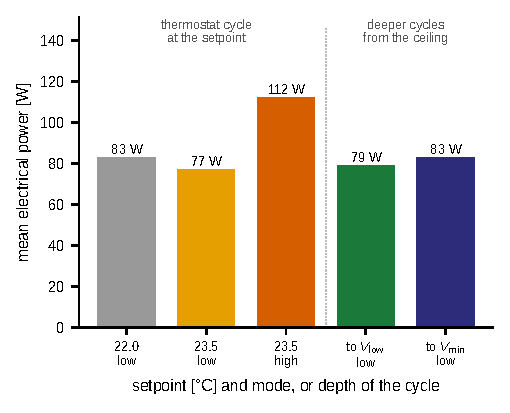
\includegraphics[width=0.8\linewidth]{fig_leap}\caption{Leap cycles of the running example (Bed~2 of apartment 2A, July, Riyadh).}\label{fig:leap}\end{figure}
\section{Validation details}\label{S:validation}\label{app:S5}
This appendix gives the details of the comparative tests of Section~\ref{sec:validation}: the BESTEST-style test on the single-zone cases of Standard~140 and the settings of the storey-box comparison with EnergyPlus.

\paragraph{BESTEST-style comparative test.} The engine of the model was run on the single-zone cases 600 (lightweight) and 900 (heavyweight) of Standard~140, with their geometry, constructions, $12\,\text{m}^2$ of south glazing, $200\,$W of internal gains, $0.5\,$ACH and the $20$/$27\,^{\circ}$C setpoints, and with the units switched off (600FF and 900FF), on the Riyadh weather instead of the standard's Denver file. The same cases were run in EnergyPlus~26.1 (Table~\ref{S:bestest}). This is a comparative test between two programs on the same inputs rather than the standard's acceptance test, whose reference ranges apply only to Denver. Cases 640 and 940 add the standard's night heating setback ($10\,^{\circ}$C from 23:00 to 07:00), which exercises the response of light and heavy construction to a setback. Free-floating, the mean temperature differs by $-1.2$ and $-1.3\,$K and the annual maximum by $-5.5$ and $-4.5\,$K. The engine therefore reproduces EnergyPlus's annual cooling closely but its peaks and extremes less closely: its exterior surfaces have a fixed film coefficient and no surface temperature of their own, and its structure is one node, so it damps the sharpest afternoon peaks. Heating is small in Riyadh, and its differences are a few hundred kWh.

\begin{table*}[t]
\centering\footnotesize\setlength{\tabcolsep}{3pt}
\caption{BESTEST-style comparative test (Standard~140 cases on the Riyadh weather; differences computed from unrounded values): annual heating and cooling [MWh], peak hourly heating and cooling [kW], and the free-floating minimum, mean and maximum temperature [$^{\circ}$C]. Cases 640/940: 600/900 with the night heating setback. E+: EnergyPlus~26.1; this: the engine of the model.}
\label{S:bestest}
\begin{tabularx}{\textwidth}{l *{8}{C}}
\toprule
 & \multicolumn{2}{c}{Case 600} & \multicolumn{2}{c}{Case 900} & \multicolumn{2}{c}{Case 640} & \multicolumn{2}{c}{Case 940} \\
\cmidrule(lr){2-3}\cmidrule(lr){4-5}\cmidrule(lr){6-7}\cmidrule(lr){8-9}
 & E+ & this & E+ & this & E+ & this & E+ & this \\
\midrule
Heating [MWh] & 0.40 & 0.62 & 0.00 & 0.01 & 0.16 & 0.28 & 0.00 & 0.00 \\
Cooling [MWh] & 11.12 & 11.10 & 9.62 & 10.04 & 11.05 & 11.04 & 9.62 & 10.03 \\
Peak heating [kW] & 1.38 & 1.63 & 0.26 & 0.57 & 3.30 & 3.77 & 0.25 & 1.05 \\
Peak cooling [kW] & 6.57 & 5.83 & 4.02 & 3.60 & 6.57 & 5.83 & 4.02 & 3.60 \\
\midrule
 & \multicolumn{2}{c}{Case 600FF} & \multicolumn{2}{c}{Case 900FF} & & & & \\
Minimum [$^{\circ}$C] & 12.0 & 9.6 & 20.2 & 19.0 & & & & \\
Mean [$^{\circ}$C] & 39.1 & 37.9 & 39.2 & 37.9 & & & & \\
Maximum [$^{\circ}$C] & 71.1 & 65.6 & 51.6 & 47.1 & & & & \\
\bottomrule
\end{tabularx}
\end{table*}

\paragraph{Settings of the storey-box comparison.} EnergyPlus runs with $10$-minute time steps, its default conduction-transfer-function heat balance and surface convection algorithms, full exterior solar distribution and the same TMYx files as the model (Riyadh Air Base, WMO 404380, record 1958--2022; Jeddah King Abdulaziz International Airport, WMO 410240, record 1981--2025). On the storey box the internal gains of the two programs are identical and their infiltration gains differ by $2.1$--$12.5$\%. Their window solar gains are not defined alike: the engine's is the total solar heat gain through the SHGC, whereas the EnergyPlus output used is the transmitted solar radiation, which leaves out the absorbed share that flows inward; the engine's is $20$--$58$\% larger. The agreement in delivered cooling therefore does not show that every heat-gain component agrees, and part of it may come from compensating differences, such as the engine's fixed exterior film coefficient and one-node structure; the engine on the storey-box geometry finds an envelope effect of $53.6\%$ in Riyadh and $53.0\%$ in Jeddah, between those of EnergyPlus and of the room-resolved model.

\section{Full sensitivity analysis and pre-cooling robustness}\label{S:sensitivity}\label{app:S6}
This appendix gives the full one-at-a-time sensitivity analysis of Section~\ref{sec:sensitivity} (all variants in the repository, \path{results/csv/repository/sensitivity_all_variants.csv}; Table~\ref{tab:robust} shows the decisive rows), the diagnostics behind it (sizing margin, controller resolution and humidity), the seasonal operation of the building, every test instance, and the stress tests of the pre-cooling result. All runs are of the whole building (Case~3); the sensitivity variants and the robustness tests are of the SBC-compliant building.

\paragraph{Every variant.} The full table, in the repository, lists for each of the 37 variants and both cities the HVAC energy intensity, the setpoint lever, the best admissible pre-cool and the cost of a $2\,$K pre-peak pre-cool, in the columns of Table~\ref{tab:robust}. Over the zone-model variants the setpoint lever spans $8.0$--$12.6$\% and the $2\,$K pre-peak cost $1.8$--$6.7$\%; over the controller and COP-model variants the setpoint lever spans $8.1$--$14.0$\% and the $2\,$K pre-peak cost $2.0$--$5.1$\%; over the equipment variants the setpoint lever spans $8.8$--$12.8$\% and the $2\,$K pre-peak cost $2.1$--$5.2$\%; over the envelope and air variants the setpoint lever spans $9.5$--$17.0$\% and the $2\,$K pre-peak cost $3.1$--$4.6$\%; over the weather variants the setpoint lever spans $9.7$--$12.2$\% and the $2\,$K pre-peak cost $3.1$--$4.6$\%. The setpoint lever is largest in the variant ``ground slab without soil resistance, constant ground temperature'' ($17.0\%$, Riyadh) and smallest in the variant ``one node, COP independent of indoor air'' ($8.0\%$, Jeddah); the pre-peak cost is largest in the variant ``one node per zone'' ($6.7\%$, Jeddah) and smallest in the variant ``one node, COP independent of indoor air'' ($1.8\%$, Riyadh). The ground variant is a bound on ground coupling rather than an alternative estimate: it replaces the ISO~13370 slab transmittance ($0.40\,$W/m\textsuperscript{2}K) by the U-value of the slab alone ($2.77$), without the soil resistance, and the monthly ground temperature by a constant $26\,^{\circ}$C in Riyadh and $29\,^{\circ}$C in Jeddah, close to the annual means of the record. The ground floor then gains heat from the warm soil all year, which raises Jeddah's HVAC energy intensity to $42.2\,$kWh/m\textsuperscript{2}yr and Riyadh's setpoint lever to $17.0\%$, while no pre-cooling setting saves. The HVAC energy intensity of the admissible variants spans $20.9$--$33.4$ in Riyadh and $30.4$--$52.4$\,kWh/m\textsuperscript{2}yr in Jeddah. The variant ``sized by load with a $15\%$ margin'' is inadmissible (Section~\ref{sec:sensitivity}).

\paragraph{Sizing margin.} Units sized by load are sized at a multiple of each room's peak hourly load on the sampled days; of the margins tried in turn ($1.15, 1.5, 2, 2.5$), the first at which every room stays within the safe set is $2.5$ in both cities. A finer sweep of the margin ($1.15$, $1.25$, $1.5$, $1.75$, $2$, $2.5$, $3$) shows what it buys. At the margins that keep every room within the safe set ($2.5$, $3$) the units save $15.5$--$16.5$\% in Riyadh and $10.6$--$11.2$\% in Jeddah against the catalogue units; the smaller margins are inadmissible, and only their excursion is reported: it falls from $69\,\mathrm{K{\cdot}h}$ in Riyadh and $18\,\mathrm{K{\cdot}h}$ in Jeddah at $1.15$ to zero from $2.5$ on, so the smallest margin that keeps every room within the safe set lies between $2$ and $2.5$. Every unit is at the $0.75$-ton minimum size at $1.15$, so the building needs $45$ tons at $1.15$ and $63$--$66$ at $3$: in capacity the margins differ far less than their names suggest. The excursions are small (the warmest room peaks at $24.15$\,$^{\circ}$C) and occur mostly in the guest rooms ($98$--$100$\% of the excursion at the tightest margin). As in the hard instances of Section~\ref{sec:generalisation}, they arise while a running unit escalates from a lower mode, not at start-up; Sections~\ref{sec:tolerance} and~\ref{sec:scope} discuss what this implies for the margin. The change of compressor, which the 3-ton variant measures on its own, accounts for most of the difference between the units sized by load as inverter units ($16.5\%$ in Riyadh and $11.2\%$ in Jeddah against the catalogue units) and with the fixed-speed zones keeping fixed-speed units ($2.1\%$ in Riyadh and $0.2\%$ in Jeddah), although the two effects are not additive.

\paragraph{Controller resolution.} The units start on average $2.0$ (Riyadh) and $2.6$ (Jeddah) times per hour of the year, a rate set by the $3$-minute time step rather than by a measured cycle; without the $3$-minute restart delay the bill changes by less than $0.01\%$. The twelve fixed-speed 3-ton units run $3$--$6$\% of the time and, as inverter units, would use $39$\% less; the four stair units, a feature of the building studied rather than of every Saudi apartment block, take $8.9$--$9.1$\% of the units' electricity and are billed to the common meter. The robustness tests below show how far a $1$-minute step, minimum on- and off-times and a cycling loss charged per start move the results.

\paragraph{Humidity.} The main model prices the latent load at a fixed latent COP and assumes the indoor target is met. A diagnostic humidity balance per zone tests that assumption: moisture enters with infiltration and from five occupants per dwelling, and the coil removes it at a given sensible heat ratio while the unit runs. In Riyadh the target holds: the conditioned rooms exceed $60\%$ relative humidity in $0.8\%$ of the cooling-season hours. In Jeddah the sensible runtime of the oversized units is too short: at a sensible heat ratio of $0.75$ the rooms exceed $60\%$ in $41\%$ of the hours ($21\%$ at $0.65$), and the coil removes $82\%$ of the latent load, so holding the target needs dedicated dehumidification, whose electricity the latent term prices. Internal latent gains would add $0.2\%$ (Riyadh) and $3.2\%$ (Jeddah) to the HVAC energy under every schedule, leaving every absolute saving unchanged. A $30\%$ lower latent COP whenever the units are off or in the lowest mode raises Jeddah's latent share to $33\%$ and leaves the scheduling result unchanged. Run for the levers themselves (current practice, the reference setpoint and $2\,$K of pre-peak or night pre-cooling), the diagnostic hardly moves: at a sensible heat ratio of $0.75$ the rooms exceed $60\%$ in $0.7$--$0.9$\% of the cooling-season hours in Riyadh and $41.1$--$44.6$\% in Jeddah. At that ratio the higher setpoint lowers the Jeddah share slightly, since warmer air holds the same moisture at a lower relative humidity, while at $0.65$ it raises it by $1.3$ percentage points. Pre-peak pre-cooling raises it at both ratios, the coil then removing $76\%$ of the latent load instead of $82\%$. The setpoint lever therefore costs little humidity comfort and pre-cooling gains none.

\paragraph{Seasonal operation.} The model runs through the whole year with units that cool and heat (Table~\ref{S:seasons}). In Riyadh summer accounts for $61\%$ of apartment 2A's HVAC energy and winter for $4\%$; Jeddah spreads its load more evenly ($47\%$ and $13\%$). The SBC-compliant building needs little heating (Section~\ref{sec:reslatent}), because its internal gains and its neighbours keep most rooms above the heating setpoint. At the reference policy no conditioned room of the SBC-compliant building leaves the safe set in either season (cold excursion $0\,\mathrm{K}\cdot\mathrm{h}$ in both cities). Over the year the units of the SBC-compliant building run in the medium or high mode in $4.5$--$5.2$\% of the hours, the fixed-speed units, which run only at full capacity, counted as high (Table~\ref{S:seasons}).

\begin{table}[t]
\centering\footnotesize\setlength{\tabcolsep}{3pt}
\caption{Summer and winter operation of the whole building at the reference policy: annual cooling, heating and latent electricity [kWh], and the share of time [\%] the units of the conditioned rooms spend off and in the low, medium and high modes, given as off/low/medium/high (cooling and heating together; fixed-speed units count as high) in summer (Jun--Sep) and winter (Dec--Feb). The remainder of the HVAC energy is the units' standby electricity, 1{,}577\,kWh a year in the SBC-compliant building. Last row: summer / winter shares of apartment 2A's HVAC energy.}
\label{S:seasons}
\begin{tabularx}{\linewidth}{@{}X r r r r@{}}
\toprule
 & \multicolumn{2}{c}{Riyadh} & \multicolumn{2}{c}{Jeddah} \\
\cmidrule(lr){2-3}\cmidrule(lr){4-5}
 & SBC & Pre-code & SBC & Pre-code \\
\midrule
Cooling [kWh] & 47{,}383 & 103{,}038 & 54{,}784 & 116{,}870 \\
Heating [kWh] & 1{,}367 & 11{,}116 & 0 & 0 \\
Latent [kWh] & 185 & 185 & 19{,}551 & 19{,}551 \\
Summer modes [\%] & 59/33/1/7 & 40/32/15/13 & 63/31/0/6 & 44/32/13/12 \\
Winter modes [\%] & 97/2/0/1 & 81/14/1/5 & 82/14/0/4 & 75/18/2/6 \\
Apt.~2A summer/winter [\%] & 61.0/3.9 & -- & 46.8/12.6 & -- \\
\bottomrule
\end{tabularx}
\end{table}

\paragraph{Test instances.} Every test instance is listed in the repository (\path{results/csv/repository/test_instances_all.csv}); Table~\ref{tab:instances} reports the eight instances with the catalogue units in one row, with their ranges, and the four hard instances one by one. With the catalogue units, the HVAC energy intensity (ranges over the two cities) is $25.1$--$37.7$ (SBC, TMYx), $32.5$--$46.0$ (SBC, heat wave), $57.5$--$68.5$ (pre-code, TMYx) and $72.2$--$89.1$ (pre-code, heat wave)\,kWh/m\textsuperscript{2}yr, and the peak load ratio is $0.19$--$0.26$ (SBC) and $0.53$--$0.62$ (pre-code). Of the $49$ lattice policies, all $49$ are admissible in the SBC building and $30$--$42$ in the pre-code building, and the best is no pre-cooling in all eight. The four tightly sized instances have peak load ratios of $0.58$, $0.57$, $0.79$ and $0.75$ (SBC Riyadh, SBC Jeddah, pre-code Riyadh, pre-code Jeddah), an annual excursion above the ceiling of $68.6$, $17.8$, $81.2$ and $28.7$\,K$\cdot$h in the same order, a warmest room of at most $24.2\,^{\circ}$C, no admissible lattice policy, and an HVAC energy intensity $13.3$--$19.5$\% below that of the catalogue units; at $23\,^{\circ}$C every one of them is admissible.

\paragraph{Robustness of the pre-cooling result.} Table~\ref{S:precoolrobust} collects these stress tests (SBC-compliant building, Case~3). None of them saves, except the favourable combinations, which need every favourable choice at once and save at most $0.77\%$. The loss per start is the unit's full power for $1.5\,$min at each start of a fixed-speed unit and for $0.82\,$min at each start of an inverter unit, calibrated to the part-load factor at the cyclic rating point; the controller variants move the absolute bill by $2$--$32$\%, the loss per start most, but not the sign of pre-cooling. With minimum on- and off-times the variant is inadmissible in Riyadh: its reference policy exceeds the ceiling from December to February, within the heating months (November to March), when the oversized fixed-speed units, held on for $3$ minutes while heating, overshoot it ($636$\,K$\cdot$h a year). The scaling to EnergyPlus multiplies the heat term of each $2\,$K run of Table~\ref{tab:precooldecomp} by the ratio $r$ of the extra heat that EnergyPlus and the engine find for the same setback on the storey box (Table~\ref{tab:setback}; $r$ is $0.75$--$0.83$) and holds the change in mean COP, so that a bill change $\Delta\Pi$ with a heat change $\Delta H$ becomes $(1+\Delta\Pi)(1+r\Delta H)/(1+\Delta H)-1$; the values are stored in the repository (\path{results/derived/energyplus_scaled_precool.json}). Scaled in this way, a $2\,$K night pre-cool still costs $3.2\%$ in Riyadh and $3.3\%$ in Jeddah. With the favourable choices combined, the best ramped setback lowers the bill by $0.55\%$ in Riyadh and raises it by $0.29\%$ in Jeddah; with the $0.08\%$ of the one-node variant whose COP ignores the room temperature (Table~\ref{tab:robust}), these rows hold the only savings found for thermostat pre-cooling. No policy cools a room of the SBC-compliant building below the $20\,^{\circ}$C floor; in the pre-code building, on the sampled days, 7 (Riyadh) and 13 (Jeddah) of the $49$ policies are inadmissible and are excluded. Of these, 7 in Jeddah let rooms drift below the floor on cool nights, by at most $0.2\,$K$\cdot$h a year and to $19.9\,^{\circ}$C, and the remaining 7 in Riyadh and 6 in Jeddah pass the ceiling. The cheapest admissible policy remains no pre-cooling.

\begin{table}[t]
\centering\footnotesize\setlength{\tabcolsep}{4pt}
\caption{Robustness of the thermostat pre-cooling result (SBC-compliant building, Case~3, volume tariff). Best: saving of the cheapest admissible policy against no pre-cooling [\%] (positive: saves; $0$: no pre-cooling is best; negative: every depth run costs, for the rows that do not include no pre-cooling among their options; --: not run, or inadmissible because the reference policy leaves the safe set). $2\,$K: change in the annual bill of a $2\,$K pre-peak pre-cool [\%] (positive: costs). Favourable choices: one node per zone, COP independent of the indoor air, inverter units in their lowest mode, no cycling loss. Dawn setback: all $365$ days; the other rows: sampled year.}
\label{S:precoolrobust}
\begin{tabularx}{\linewidth}{@{}X r r r r@{}}
\toprule
 & \multicolumn{2}{c}{Riyadh} & \multicolumn{2}{c}{Jeddah} \\
\cmidrule(lr){2-3}\cmidrule(lr){4-5}
Test & Best & $2\,$K & Best & $2\,$K \\
\midrule
Base model, lattice of $49$ policies & $+0.00$ & $+3.40$ & $+0.00$ & $+4.30$ \\
Inverter units in lowest mode & $+0.00$ & $+1.95$ & $+0.00$ & $+2.84$ \\
Ramped pre-peak setback ($0.5\,$K/h) & $-0.25$ & $+2.26$ & $-0.34$ & $+3.04$ \\
Extra heat scaled to EnergyPlus & -- & $+2.94$ & -- & $+3.82$ \\
Dawn setback, $2\,$K, all $365$ days & $-0.99$ & -- & $-1.80$ & -- \\
Top floor only (15 units) & $+0.00$ & $+0.82$ & $+0.00$ & $+1.14$ \\
Rooms with west windows only (12 units) & $+0.00$ & $+1.02$ & $+0.00$ & $+1.29$ \\
Cycling loss charged per start & $+0.00$ & $+2.45$ & $+0.00$ & $+2.82$ \\
$1$-minute step & $+0.00$ & $+2.11$ & $+0.00$ & $+2.85$ \\
$1$-minute step, $3$-min minimum on/off, loss per start & -- & -- & $+0.00$ & $+2.45$ \\
Favourable choices combined & $+0.77$ & $-0.21$ & $+0.03$ & $+3.07$ \\
Favourable choices, top floor only & $+0.21$ & $-0.20$ & $+0.00$ & $+0.50$ \\
\bottomrule
\end{tabularx}
\end{table}

\section{Uncertainty analysis}\label{S:uq}\label{app:S7}
Seventeen assumed inputs of the SBC-compliant building (Case~3, sampled year) are varied jointly over the uniform ranges of Table~\ref{S:tab:uqpar} by a Latin hypercube of $128$ samples per city (fixed seed). This appendix gives the input ranges and the partial rank correlations; the per-sample inputs and results are not reproduced here but are in the repository (\texttt{results/parts/uncertainty\_Riyadh.json} and \texttt{uncertainty\_Jeddah.json}). For each sample the reference, current-practice and $0.5$--$2\,$K pre-cooling policies (night or pre-peak), the pre-code building and the 3-ton units as inverter units are simulated. The weather inputs scale the daily swing of the air temperature about each day's mean and shift it uniformly (the heating months follow the shifted weather). The PRCC of every input with every result are in the repository (\path{results/csv/repository/uncertainty_prcc.csv}). The strongest partial rank correlations (Riyadh/Jeddah, ranked by the larger magnitude of the two) are as follows. For the setpoint lever they are the indoor COP slope $\gamma$ ($+0.93$/$+0.98$), the infiltration ($-0.85$/$-0.57$) and the latent COP ($-0.10$/$+0.84$). For the envelope lever they are the infiltration ($-0.88$/$-0.96$), the internal-gain scale ($-0.90$/$-0.77$) and the opaque solar absorptance ($+0.85$/$+0.87$). For the inverter lever they are the fixed-speed $C_d$ ($+0.94$/$+0.95$), the COP ratio $c_1/c_3$ ($+0.90$/$+0.89$) and the inverter $C_d$ ($-0.89$/$-0.89$). For the cost of a $2\,$K pre-peak pre-cool they are the indoor COP slope $\gamma$ ($+0.69$/$+0.65$), the air-node share of capacitance ($-0.44$/$-0.46$) and the inverter $C_d$ ($-0.37$/$-0.38$). For the cost of a $2\,$K night pre-cool they are the indoor COP slope $\gamma$ ($+0.76$/$+0.81$), the outdoor COP slope ($-0.78$/$-0.80$) and the infiltration ($+0.55$/$+0.15$). The best admissible pre-cool is zero in every sample and so has no rank correlation; the coefficients of all 17 inputs with every result are in the repository file.

\begin{table}[t]
\centering\footnotesize
\caption{Inputs of the uncertainty analysis: base value and uniform range.}\label{S:tab:uqpar}
\begin{tabularx}{\linewidth}{@{}X r r r@{}}
\toprule
Input & Base & Low & High \\
\midrule
indoor COP slope $\gamma$ & $0.02$ & $0$ & $0.03$ \\
outdoor COP slope & $0.02$ & $0.01$ & $0.03$ \\
COP ratio $c_1/c_3$ & $1.45$ & $1.3$ & $1.6$ \\
COP ratio $c_2/c_3$ & $1.24$ & $1.1$ & $1.3$ \\
inverter $C_d$ & $0.15$ & $0.05$ & $0.25$ \\
fixed-speed $C_d$ & $0.25$ & $0.15$ & $0.35$ \\
escalation-threshold scale & $1$ & $0.5$ & $2$ \\
air-node share of capacitance & $0.05$ & $0.02$ & $0.15$ \\
latent COP & $3.4$ & $2.5$ & $4$ \\
infiltration & $0.4$ & $0.2$ & $0.8$ \\
internal-gain scale & $1$ & $0.7$ & $1.3$ \\
wall $U$ (thermal bridges) & $1$ & $1$ & $1.2$ \\
opaque solar absorptance & $0.7$ & $0.5$ & $0.9$ \\
door exchange (scale) & $1$ & $0.5$ & $1.5$ \\
capacity derating slope & $0.01$ & $0.005$ & $0.02$ \\
daily temperature swing (scale) & $1$ & $0.8$ & $1.3$ \\
air temperature shift [K] & $0$ & $-1$ & $2$ \\
\bottomrule
\end{tabularx}
\end{table}


\bibliographystyle{unsrtnat}
\ifnum\blindmode=1 \bibliography{references_blind}\else \bibliography{references}\fi

\end{document}

